\documentclass[11pt,a4paper,twoside,openright]{report}

% Document based upon the 'Report' class. 
% Uses 11pt text in standard font families, paper size is globally set to A4, the PDF will be laid out as a two-sided 
% document (allows different margins on odd/even pages for later binding) and its first page will be a right page. 

\includeonly{%		% comment out lines to not compile these sections when typesetting. 
	%%Preface
	./Preface/frontspace,
	./Preface/copyright,%
	./Preface/dedication,%
	./Preface/toc,%
	./Preface/acknowledgements,%
	./Preface/abstract,%
%	./Preface/sommario,%
	%
	%%Body
	%
	./chapters/intro,%
	./chapters/materials,%
	./chapters/synthesis,%
	./chapters/characterization,%
	./chapters/fabrication,%
	./chapters/dataAnalysis,%
	./chapters/results,%
	./chapters/conclusion,%
	./chapters/appendix
	}

%%%%%%%%%%%%%%%%%%%%%%%%%%%%%%%%%%%%%%%%%%
%%%%%%%%%% PACKAGE MANAGEMENT %%%%%%%%%%%%%%%%%%
%%%%%%%%%%%%%%%%%%%%%%%%%%%%%%%%%%%%%%%%%%

\usepackage{soul}
\usepackage{color}
\usepackage{tocloft}
\usepackage{graphicx}	% Package for using images (.jpg, .pdf, .png, etc.) as figures. 
\usepackage[center]{caption}	% Captioning packages for floats (figures, tables, etc.). '[Center]' forces centering
\usepackage{subfig}
%\usepackage{subcaption}	% Allows for sub-figures to have their own sub-captions, shouldn't be in TOC
\usepackage{tabularx} % Allows for automatic sizing for tabular environments (see CTAN for manual)
\usepackage[super]{cite}	% Automatic citation generation package '[super]' forces superscript citations
\usepackage{afterpage}	% Package to be used with \clearpage to help keep floats from drifting to end of document. (See CTAN for manual)
%\usepackage[version=3]{mhchem}	% Automatic formatting of chemical equations and formulas
\usepackage[method=mhchem]{chemmacros}
\usepackage{amsmath,amssymb,mathtools}	%Packages for various equation tools
\usepackage{rotating}	% Allows rotation of objects (figures, tables, etc.). Preferable to use landscape environment in most cases (\begin{lscape})
\usepackage{xnewcommand}
\usepackage{siunitx}
\usepackage{setspace}
\usepackage{fancyhdr}	% Package for setting up headers and footers
\usepackage[english]{babel}	% Language setting, not sure why its necessary, but is.
\usepackage[nodayofweek]{datetime}	% Allows for proper determination of date
\usepackage{etoolbox} 	% Unimportant for end user. 
\usepackage{lipsum}	% Allows for automatic creation of filler text. 
\usepackage[inner=1.5in,outer=1in,top=1in,bottom=1in,pdftex]{geometry} % Defines page layout geometry
\usepackage{lscape}	% Allows pages to be defined as landscape (environment)
\usepackage{indentfirst}	% Forces an indent on all paragraphs, including first paragraphs. 
\usepackage{empheq}	% Used to add braces to groups of equations
\usepackage[running,modulo]{lineno}	% Adds line numbers (only multiples of 5) to left side margin
\usepackage{varioref}
\usepackage{multirow}
\usepackage{longtable}
\usepackage{booktabs}
\usepackage{arydshln}

% Hyperref package: used for setting up hyperlinks in the document (TOC, citations, figures, equations, etc.), as 
% well as adding PDF metadata (author, title, etc.)
\usepackage[pdftex,%	Informes explicitly use of pdftex for document preparation engine
		      hyperfigures, % 	Requests hyperlinks from figure citations to their associated figures
		      pageanchor=true,% 	Necessary for proper hyperlinking of TOC
		      %pagebackref=true,%
		      hyperindex=true,%	If index is present, entries will link back to the first appearance of the term
		      colorlinks=true,	%	Colors links in document (internal: red, citations: green)
		      citecolor=green,%
		      bookmarks=true,%	Creates bookmarks list in the final PDF
		      bookmarksnumbered=true,%	Adds chapter number to the associated bookmark
		      bookmarksopen=true,%	All bookmark trees open when PDF opened, not working
		      pdftitle={A Method for Atomic Layer Deposition of Complex Oxide Thin Films},%	Document title
		      pdfauthor={Brian R. Beatty},%	Document author
		      pdfsubject={M.S. Thesis},%	Document subject
		      pdfkeywords={ALD, Atomic Layer Deposition, Ferroelectric, Complex Oxide, Perovskite, %
		      Lead Titanate, Lead Zirconate Titanate, PbTiO3, PTO, PT, PZT, Thin Film, Epitaxy},
		      %List of keywords for document
		      ]{hyperref}	


%%%%%%%%%%%%%%%%%%%%%%%%%%%%%%%%%%%%%%%%%%
%%%%%% ADJUSTS CHAPTER TITLES CLOSER TO HEADER   %%%%%%%%%
%%%%%%%%%%%%%%%%%%%%%%%%%%%%%%%%%%%%%%%%%%

\makeatletter
% "\@makechapterhead" applies to ordinary or numbered chapters
\patchcmd{\@makechapterhead}{\vspace*{50\p@}}{}{}{}
\patchcmd{\@makechapterhead}{\vskip 40\p@}{\vskip 20\p@}{}{}
% "\@makeschapterhead" applies to "starred" or un-numbered chapters
\patchcmd{\@makeschapterhead}{\vspace*{50\p@}}{}{}{}
\patchcmd{\@makeschapterhead}{\vskip 40\p@}{\vskip 20\p@}{}{}


\widowpenalty=7500
\clubpenalty=7500

\let\origtableofcontents\tableofcontents
\renewcommand{\tableofcontents}{%
  \begingroup
  \renewcommand*{\contentsname}{Table of Contents}
  \origtableofcontents
  \endgroup}

\renewcommand{\@cftmaketoctitle}{%
   {\interlinepenalty\@M
        \par\nobreak
        {\Huge \bfseries Table of Contents \par\nobreak}
        \par\nobreak
    \vskip 20\p@
    \thispagestyle{fancy}
  }}  
  
  \renewcommand{\@cftmakelottitle}{%
   {\interlinepenalty\@M
        \clearpage
        \par\nobreak
        {\Huge \bfseries List of Tables \par\nobreak}
        \par\nobreak
    \vskip 40\p@
    \thispagestyle{fancy}
  }}  
  
  \renewcommand{\@cftmakeloftitle}{%
   {\interlinepenalty\@M
        \clearpage
        \par\nobreak
        {\Huge \bfseries List of Figures \par\nobreak}
        \par\nobreak
    \vskip 40\p@
    \thispagestyle{fancy}
  }}  

 \setlength{\textfloatsep}{1.5em}
 \setlength{\intextsep}{1.5em}
 
\def\cleardoublepage{\clearpage\if@twoside \ifodd\c@page\else
  \thispagestyle{empty}\hbox{}
\newpage
  \if@twocolumn\hbox{}\newpage\fi\fi\fi}

{\def\thebibliography#1{\chapter*{\bibname
	\@mkboth{\bibname}{\bibname}}%
	\list{[\arabic{enumi}]}{\settowidth\labelwidth{[#1]}%
	\leftmargin\labelwidth \advance\leftmargin\labelsep
	\usecounter{enumi}}%
	\def\newblock{\hskip.11em plus.33em minus.07em}%
	\sloppy\clubpenalty4000\widowpenalty\clubpenalty
	\sfcode�\.=1000\relax}}{}
\makeatother

\renewcommand{\bibname}{List of References}
\addto{\captionsenglish}{\renewcommand{\bibname}{List of References}}


%%%%%%%%%%%%%%%%%%%%%%%%%%%%%%%%%%%%%%%%%%
%%%%%%%%%%% MISCELLANEOUS ADJUSTMENTS   %%%%%%%%%%%%
%%%%%%%%%%%%%%%%%%%%%%%%%%%%%%%%%%%%%%%%%%

\setlipsumdefault{1-2}  % Makes \lipsum automatically produce 2 paragraphs of filler text

\renewcommand{\lipsum}{} % Hide dummy text paragraphs



\renewcommand{\captionfont}{\normalfont \sffamily \itshape \small}
%\renewcommand{\contentsname}{Table of Contents}

\pagestyle{empty} % Sets pages to have no header/footer. Will be changed later in the document. 


%%%%%%%%%%%%%%%%%%%%%%%%%%%%%%%%%%%%%%%%%%
%%%%%%%%%%% LAYOUT GEOMETRY ADJUSTMENTS  %%%%%%%%%%%
%%%%%%%%%%%%%%%%%%%%%%%%%%%%%%%%%%%%%%%%%%

%\addtolength{\oddsidemargin} {-0.4 cm} 	% Shrinks the side margins slightly.
%\addtolength{\evensidemargin} {-0.4 cm}	% Shrinks the side margins slightly. 

\setlength{\headheight}{26pt} 	% Changes the size of the header (the console will complain if it's too small).

\linespread{1.25} 	% Changes line spacing



%%%%%%%%%%%%%%%%%%%%%%%%%%%%%%%%%%%%%%%%%%
%%%%%%%%%%%  CHEMICAL EQUATION FORMATTING  %%%%%%%%%%%
%%%%%%%%%%%%%%%%%%%%%%%%%%%%%%%%%%%%%%%%%%

\renewtagform{reaction}[R ]{(}{)}


%%%%%%%%%%%%%%%%%%%%%%%%%%%%%%%%%%%%%%%%%%
%%%%%%%%%  PERSONALIZED COMMANDS %%%%%%%%%%%%%%%%%
%%%%%%%%%%%%%%%%%%%%%%%%%%%%%%%%%%%%%%%%%%

% Shortcuts for typesetting certain things quickly (saves time when typing things often). 
% Always use an empty set of braces after the command unless it has arguments. 

\newcommand{\PTO}{\ce{PbTiO3}}

\newcommand{\PZT}{\ce{PbZr_{x}Ti_{1-x}O3}}

\newcommand{\Deg}{$^{\circ}$}
\newcommand{\degC}{$^{\circ}$C}
\newcommand{\Tc}{T$\mathrm{_{C}}$}

\newcommand{\TiIon}{\ce{Ti^{4+}}}
\newcommand{\OIon}{\ce{O^{2-}}}
\newcommand{\PbIon}{\ce{Pb^{2+}}}
\newcommand{\ZrIon}{\ce{Zr^{4+}}}
\newcommand{\TiOiPr}{Ti-o-\emph{i}-Pr}

\newcommand{\TMHD}{Pb(TMHD)$_{2}$}
\newcommand{\tmhd}{\TMHD}
\newcommand{\HFAc}{Pb(HFAc)$_{2}$}
\newcommand{\hfac}{\HFAc}

\newcommand{\leftstuff}[2][0pt]{\smash{\raisebox{#1}{\llap{#2}}}}

\newcommand{\reword}[1]{%
	\sethlcolor{yellow}%
	\hl{#1}%
	}

\newcommand{\rewrite}[1]{\reword{#1}}

%%%%%%%%%%%%%%%%%%%%%%%%%%%%%%%%%%%%%%%%%%
%%%%%%%%%%% DOCUMENT STARTS HERE  %%%%%%%%%%%%%%%%
%%%%%%%%%%%%%%%%%%%%%%%%%%%%%%%%%%%%%%%%%%

\begin{document} 	% Now the fun starts.

%%% PREFACE %%%
\renewcommand{\headrulewidth}{0.3pt}
{\thispagestyle{empty} % No headers/footers allowed here
%\thispagestyle{empty}
\begin{titlepage}
%\vspace*{-2.5cm}
\begin{center}
  {\Huge
  \textsc{Drexel University}\\
  \vspace{0.5em}
  \textbf{\Large
  Department of Materials Science and Engineering}}\\
  \vspace*{0.5cm}
  \begin{figure}[htbp]
    \begin{center}
      
\includegraphics[width=7cm]{./pictures/LogoPoliMi}
    \end{center}
  \end{figure}
 % \vspace{-0.5cm}
   {\huge\textsc{
  A Method for\\
  Atomic Layer Deposition\\
  of Complex Oxide Thin Films\\
  }}

  
  
\end{center}
\large
\begin{centering}
\vspace{0.2cm}
\begin{tabular*}{0.75\textwidth}{>{\bfseries}r l}
  Advisor & Dr. Jonathan E. Spanier \\
  & \emph{\tiny Drexel University, Philadelphia, Pennsylvania, United States of America}
  \vspace{0.3cm}
\end{tabular*}

\end{centering}
%\vspace*{0.5cm}
\rule{\linewidth}{0.5mm}\vspace{0.3cm}
\begin{centering}\\
  {\small{\Large\scshape A Thesis}\\Submitted to the Faculty in\\{\Large\scshape Partial Fulfillment}\\of the Requirements\\
  	for the Degree of\\{\Large\scshape Master of Science}\\by:\\}
  \vspace*{0.5em}\textbf{\LARGE Brian R. Beatty}\vspace*{0.5em}
  %\small Student ID \#11404903 \\ 
%\vspace*{1em}
\rule{\linewidth}{0.5mm}

\end{centering}
%\vspace*{0.5cm}
\begin{center}
  Academic Year 2011-2012
\end{center} \clearpage

\end{titlepage} % Opens a sub-TEX file. ./ is the current local directory. 
}

{\cleardoublepage \normalfont   % No header/footer on this page, then starts new odd # page
\vspace*{\fill}

\begin{center}

\copyright\ Copyright \monthname\ 2012\\
Brian R. Beatty. All Rights Reserved.

\end{center}

\vspace*{\fill}}

{\normalfont \cleardoublepage
\newpage
\vspace*{4cm}
\large
\begin{flushright}
\itshape{For my parents and everyone\\else who helped out along the way...}
\end{flushright}

\cleardoublepage

\vspace*{4cm}
\large
\begin{flushright}
\itshape{You cannot teach a man anything;%
	     \\you can only help him discover it in himself.%
	     \\\vspace{0.75em} -Galileo Galilei}
\end{flushright}}
\fancyfoot[C]{\thepage}
\fancyhead{}



{\cleardoublepage
\pagestyle{fancy}
%\linenumbers			% Starts numbering of document lines
\pagenumbering{roman} %Start numbering preface pages using roman numerals (i, ii, iii, iv, ...)
%\addtocounter{page}{-2}
%\vspace*{.75truecm}
\fancyhead[RE]{\nouppercase{\bfseries\leftmark}}
\fancyhead[LO]{\nouppercase{\bfseries\rightmark}}
\fancyhead[LE,RO]{\bfseries\thepage}
\fancyfoot{}
\tableofcontents
\label{toc:ToC}
\captionsetup{lofdepth=2}

\listoffigures
\label{toc:listoffig}
\addcontentsline{toc}{chapter}{List of Figures}

\cleardoublepage
\thispagestyle{empty}
\listoftables
\label{toc:listoftbl}
\addcontentsline{toc}{chapter}{List of Tables}
%\listofreactions
%\addcontentsline{toc}{chapter}{List of Reactions}

% Uncomment below to add a list of tables. Probably necessary for sample information table. 

%\label{toc:listoftbl}
%\listoftables
%\addcontentsline{toc}{chapter}{List of Tables}}

\pagestyle{fancy}
\chapter*{Acknowledgements}
\thispagestyle{empty}

\addcontentsline{toc}{chapter}{Acknowledgements}

I would like to start by acknowledging Dr. Jonathan Spanier for all of the all of the guidance that he has given to me over the course of my tenure at Drexel University. Allowing me to enter into the research side of school as a young freshman with stars in his eyes was undeniably one of the defining points in my academic career. The variety of skills I have been able to learn while working with him, and of course all of the members of his extremely talented group, are sure to prove to be invaluable during the next stages of life after Drexel. While I learned plenty of facts and received valuable training in an incredible range of technical equipment, what really stands out is the manner in which I was taught how to think. How to think about puzzling results that didn't quite add up evenly. How best to plan experiments to maximize the data obtained from it. Analyzing the remnants from when things went wrong, and figuring out how to prevent such things from happening in the future. The researcher's mindset is one of inquisitiveness and analysis and a drive to truly understand, and it has been of great value both in and out of the laboratory. 

Another pair of honorable mentions goes to Dr. Stephen Nonnenmann and Dr. Eric Gallo. These two served me as would-be mentors as I tried to get my feet under me in my first year or so. Always around to bounce questions off of, quick with helpful advice, and utterly filled to the brim with useful knowledge. Between these two, there was nothing that couldn't get done or be answered in the lab. These two set me up with the knowledge and mental tools I would need to go off exploring on my own journeys into the wild seas of science. I cannot thank them enough. 

Then there was the rest of the stalwart crew. Stephanie Johnson, Oren Leaffer, Terrance McGuckin, Guannan Chen, and Christopher Hawley. And I couldn't forget my fellow undergrads Dominic Bruzzese and Michael Coster. The great conversations --- especially with Oren (whom I can still count on for some useful advice about any question) even if they tended to get a little long-winded at times --- that I had with these characters will be some of my best memories from my time here. Each of us had our own idiosyncrasies, but I like to think we made a fantastic team when you put us all together. 

Of course, I would also like to send a heartfelt thank you to three more individuals who worked closely with my project at three very different stages. Rahul Joseph was my mentor when I first joined the lab, and it was a derivative of his project that over time metamorphosed into the thesis sitting before you.  Dr. Greg Soja was a post-doctorate fellow who worked alongside me on this project as well, and helped solve some rather difficult problems that we encountered. Last, but far from least, is Dr. Maria Sancho-Torres. She brought a bit of spark and a new point of view to the project that, again, helped sort out some problems that otherwise might have stymied me for a lot longer than they should have. 

I must also thank Keith Fahnstock and Dr. Caroline Schauer for allowing me and helping me with the use of their ellipsometer. Keith in particular, for his training and just good conversation (both on and off topic) when data collection got boring. In the same vein, I must gratefully acknowledge the assistance that Dr. Amy Fahnstock and her advisor Dr. Giuseppe Palemese provided me by allowing access to their TGA and DSC instrumentation that was pivotal to the success of this project. 

Of course, one does not live in a bubble, and I must thank the rest of the excellent faculty of the Materials Engineering Dept. for all of their efforts (both for their informative courses, but primarily for the discussions we had outside the classroom). I feel that I need to particularly acknowledge Dr. Steve May and Dr. Antonios Zavaliangos in this regard. 

Along the lines of the opportunity I have had during this past year abroad, I would like to personally thank Dr. Carlo Casari, Politecnico di Milano, and everyone who had a hand in making the E.A.G.L.E.S. program come together. And of course the scores of crazy friends that I picked up along the way. 

This has been a lot of talk already, but I personally feel I saved the most important for last.  My father, Bruce, and my mother, Amy, deserve more thanks than I think they realize. For being the supports that I could fall back on, for sharing in both the little successes and the big triumphs, for always letting me talk about what I was working on (and oh the respect I have for trying to learn about it from me...), and for always pushing me to go beyond what I thought I was capable of. Mom and Dad, thank you so very much. This one's for you guys. Now on with the show. 












%\vspace*{.75truecm} 
\normalfont \cleardoublepage

\mbox{}\thispagestyle{empty}
\cleardoublepage
\chapter*{Abstract}
\addcontentsline{toc}{chapter}{Abstract}

%%%%%%%%%%%%%%%%%%%%%%%%%%%%%%%%%%%%%%%%%%%%%%%%%%%%
%%%%%%%%%%%%%%%%%%%%%%%%%%%%%%%%%%%%%%%%%%%%%%%%%%%%
%%%%%%%%%%%%%%%%%%%%%%%%%%%%%%%%%%%%%%%%%%%%%%%%%%%%

Advanced technologies derive many of their capabilities from the advanced materials that they are made from. Complex oxides are a class of materials which are driving technological advancement in a host of different directions. These highly functional materials have a great variety of useful properties, which can be chosen and even engineered through careful choice of material. 

Advanced materials require advanced deposition methods. Atomic layer deposition (ALD), a variant of chemical vapor deposition (CVD), is gaining more use in industry for its ability to provide ultra-high film thickness resolution (down to 0.1 nm), capability to conformally coat three-dimensional structures, and its high uniformity across large surface areas. Additionally, ALD processes provide a possibility to improve economic and environmental viability of the process as compared to CVD by using and wasting less toxic reactants and expelling fewer nano-particulate byproducts. 

ALD processes are highly mature for many binary oxides commonly used in the semiconductor industries, however processes for depositing heavy metal oxides and complex oxides --- oxides containing two or more separate metallic cations --- are sorely lacking in literature. 

The primary focus of this work is the development of a process for depositing the complex perovskite oxide lead titanate (\PTO{}), an end group of the lead zirconate titanate family (\ce{PbZr_{x}Ti_{1-x}O3}), which has valuable technical applications as well as serves as a template for applying this research into other material systems. 

The author gratefully acknowledges the Army Research Office (ARO) for their support of this project under the funding provided by Grant \# W911NF-08-1-0067.


%
%\reword{XXXXXXXXXXXXXXXX}
%
%As devices based on ferroelectric films become more commonplace, a commercially viable process for fabricating the material is needed; low cost and high volume are implied necessities for such a process. This work focuses on the application of atomic layer deposition (ALD) to this task. ALD is a standard fabrication process in the electronics industry, valuable for its high uniformity across large surfaces, capability to control film thickness with very high resolution, and conformality across three dimensional structures. The various tasks in designing and optimizing an ALD process, as well as characterization methods for analysis of the produced films, are discussed here in detail.
%
%The primary focus of this work is the development of a process for depositing lead titanate (\ce{PbTiO3}) thin films via an ALD process. Research focused on the application of bis(2,2,6,6-tetramethyl-3,5-heptanedionato)lead(II) (Pb(TMHD)$_{2}$) toward this end. 
%
%Work done towards the completion of this study was supported by the Army Research Office under Grant \#W911NF-08-1-0067. 
%\vspace*{.75truecm} 
\cleardoublepage

\newpage
\chapter*{Sommario}

\addcontentsline{toc}{chapter}{Sommario}

In questo studio, viene proposto un metodo per lo sviluppo di un nuovo processo di deposizione Atomic layer depositon (ALD) per film sottili. Questo include l�identificazione, la verifica e la selezione dei precursori; l�analisi dei parametri di crescita e dei loro effetti sui film prodotti e la caratterizzazione ex situ mediante varie tecniche.

	Il materiale in esame \`e titanato di piombo (PTO, \PTO{}), della famiglia del titanato zirconato di piombo (PZT, \PZT{}). Il titanato di piombo \`e un ossido perovskitico complesso, che presenta ferroelettricit\`a a temperatura ambiente ed ha una elevata temperatura di Curie alla quale transisce  al comportamento paraelettrico. La ferroelettricit\`a \`e una propriet\`a interessante, in quanto comporta un comportamento isteretico della polarizzazione del materiale. Questo permette al materiale di passare da uno stato all�altro e di richiamare la polarizzazione memorizzato anche senza la presenza di un campo elettrico. Questa propriet\`a \`e di interesse per una vasta gamma di applicazioni nel campo dell�elettronica e delle altre scienze fisiche. 

	Ci sono un gran numero di tecniche di deposizione per strutture a film sottile. Alcune, quali sol-gel, si basano su principi di �wet chemistry�  e consentono la formazione di film con una composizione altamente controllata. Tuttavia, tali tecniche possiedono tutti gli inconvenienti dei metodi chimici a base di soluzioni. La deposizione chimica da fase vapore (CVD) \`e un altro metodo molto comune di deposizione di film sottili. Esso ha una serie di vantaggi, come ad esempio la capacit\`a di depositare film epitassiali  (con un notevole miglioramento della qualit\`a delle interfacce). Tuttavia non \`e facile controllare con precisione lo spessore e rivestire in maniera conforme strutture non planari \`e un compito molto difficile. La ALD \`e una tecnica basata su una modifica del processo CVD. Si separa una reazione tra il precursore metallico e l�ossidante in due semireazioni. Queste semireazioni sono in grado di verificarsi solo sulla superficie del substrato e non in fase gas. La separazione  delle reazioni porta ad una serie di importanti cambiamenti. Una delle caratteristica pi\`u critiche, della deposizione ALD, \`e che la reazione diventa auto-limitante. Una semireazione puo� depositare al massimo un monostrato di materiale. Questo permette una risoluzione nel controllo dello spessore che pochissime altre tecniche possiedono. La ALD \`e in grado di controllare lo spessore fino al livello dell�angstrom (1 \AA\ = 0.1 nm). Questo comportamento autolimitante d\`a anche alla ALD alcuni altri vantaggi, quali la possibilit\`a di rivestire con precisione e in modo conforme una struttura complessa tridimensionale mantenendo la stessa risoluzione. Questo \`e quasi impossibile con qualsiasi altro processo di deposizione. I precursori usati nella ALD sono pi\`u particolare di quelli tipici per CVD. Essi devono essere reattivi con la superficie e con un ossidante, ma non devono essere in grado di reagire tra dio loro. La temperatura necessaria per attivare la reazione con la superficie deve essere inferiore alla temperatura di pirolisi necessaria per rompere la molecola. Infine, al termine di ciascuna coppia di semireazioni  \`e necessario ripopolare i siti superficiali con i ligandi appropriati capaci di reagire con il precursore. Un precursore per ALD comunemente usato per il titanio \`e il titanio(IV) isopropossido, mentre  se non esiste un precursore ALD ideale per il piombo. Di una serie di due diversi composti sono stati scelti per ulteriori indagini il bis (2,2,6,6-tetrametil-3 ,5-heptanedionato) piombo (II) (\TMHD{}) e piombo(II) hexafluoroacetylacetonate (\HFAc{}). I due precursori selezionati sono stati analizzati utilizzando analisi termo gravimetrica (TGA) e calorimetria a scansione differenziale (DSC). Tra le due tecniche \`e stato possibile identificare le regioni di volatilit\`a ideale e un intervallo di temperatura in cui potrebbe avvenire le reazioni potenzialmente vitali per il processo ALD. Da questa analisi, ci si aspettava che \TMHD{} si comporta meglio di \HFAc{} in un processo di ALD. 

	Alcuni campioni sono stati preparati ed analizzati. La ellissometria spettroscopica ad angolo variabile\`e stata utilizzata per misurare gli spessori dei film e i tassi di crescita, insieme ad alcune propriet\`a ottiche ed elettroniche. La spettroscopia di fluorescenza a raggi X (XRF) \`e stata utilizzata per ottenere analisi compositive quantitative sui campioni. La diffrazione di raggi X (XRD) \`e stata utilizzata per studiare le fasi presenti e la loro relativa concentrazione nei campioni finali. A conclusione di questo studio, si \`e scoperto che \`e possibile far crescere ossidi di perovskite complessi tramite ALD, ma di ottenere campioni cristallizzati di pura fase perovskite  non \`e banale e richiede ulteriori studi. Tuttavia, durante questo lavoro di tesi si \`e riuscito a sviluppare una procedura importante per lo sviluppo di processi ALD di vari materiali. Ulteriori lavori comprendono l�analisi del comportamento ferroelettrico dei film, migliorare la purezza di fase nei campioni finali, e l�estensione del metodo di deposizione per creare sistemi di altro materiale come \PZT{} o titanato di stronzio e bario ((Ba,Sr)Ti\ce{O3}).

%\vspace*{.75truecm}
\cleardoublepage

%%% END OF PREFACE %%%
\fancyhead[]{}
\fancyfoot{}
  % Start numbering pages using arabic numerals (1, 2, 3, 4, ...)


%%%%%%%%%%%%%%%%%%%%%%%%%%%%%%%%%%%%%%%%%%
%%%%%%%%%%% HEADER/FOOTER SETUP  %%%%%%%%%%%%%%%%%
%%%%%%%%%%%%%%%%%%%%%%%%%%%%%%%%%%%%%%%%%%

\pagestyle{fancy} 	% Activates fancyhdr package to make customized headers/footers. 

\renewcommand{\chaptermark}[1]{\markboth{\chaptername\ \thechapter :\ #1}{}} % Changes definitions for chapter titles in header
\renewcommand{\sectionmark}[1]{\markright{\thesection :\ #1}}         % Changes definitions for section titles in header

 % Changes geometry settings

\fancyhead[LE,RO]{\bfseries\thepage}    % Page number will be bold and appear on the left side on even pages (LE) and the right side on odd pages (RO).
                                        
\fancyhead[RE]{\bfseries\leftmark}    % Uses default settings for right page headers (chapter number and title)
\fancyhead[LO]{\bfseries\rightmark}     % Uses default settings for left page (section number and title
\renewcommand{\headrulewidth}{0.3pt}

\clearpage
\thispagestyle{empty}
\mbox{}
\cleardoublepage

%%% BEGIN CONTENT %%%

% Each chapter located in its own sub-file to make it easier to work on them. NOTE: they will not compile on their own. 
% To view the result, you need to run TeX on the main document (thesis.tex). Can be done by clicking on the open 
% PDF and pressing command-T. 

% NOTE: 	To get references (to figures and such) to update properly, TeX must be run TWICE. 
% 	 	To get citations to work properly, you must run: TeX (cmd-T), BibTeX (cmd-shft-B), TeX, TeX. (4 total runs)
\pagenumbering{arabic}
\chapter{Introduction}
\label{ch:Intro}
\thispagestyle{empty}


%%%%%%%%%%%%%%%%%%%%%%%%%%%%%%%%%%%%%%%%%%%%%%%%%%%
%%%%%%%%%%%%%%%%%%%%%%%%%%%%%%%%%%%%%%%%%%%%%%%%%%%
%%%%%%%%%%%%%%%%%%%%%%%%%%%%%%%%%%%%%%%%%%%%%%%%%%%

Modern technology stands on the shoulders of modern materials, and the two are inextricably linked together. Whenever a new material or property has been discovered or engineered, applications of this new capability lie just over the horizon. 

One of the areas of rapid innovation and great interest in novel applications of material properties is the field of oxide chemistry. Such a seemingly simple class of materials, examples of which are two of the most abundant compounds on Earth (i.e. silica and alumina), has an incredibly rich set of capabilities derived from the incredible variety of potential materials. One example is the field of high-\textsc{k} dielectric oxides, such as hafnium oxide (\ce{HfO2}) and zirconium oxide (\ce{ZrO2}),\cite{chen_atomic_2007,fischer_batch_2008} which are allowing the semiconductor industry to produce more capable devices while reducing power draw. Ferromagnetic and antiferromagnetic oxides form the basis of the ubiquitous magnetic hard disk drive, advancements in deposition and microstructure control allow for the steady increase in capacities that consumers have become accustomed to.\cite{scheffe_atomic_2009}

The class of ferroelectric oxides comprises the family of materials that this thesis will consider. One material in particular will be the primary subject: lead titanate (PTO, \PTO{}).\cite{harjuoja_2006,lee_effects_2009} Lead titanate is one end group of the lead zirconate titanate family of ferroelectric oxides (PZT, \ce{PbZr_{1-x}Ti_{x}O3}).\cite{Muralt_2000} The PZT family is of particular technical importance to many applications, especially the \ce{PbZr_{0.52}Ti_{0.48}O3} form which exhibits exemplary piezoelectric, ferroelectric, and pyroelectric behavior. PZT's piezoelectric capabilities allow for it to be used as actuators and sensors in innumerable devices (e.g. tip actuators in AFM microscopes and transducers in ultrasound imagers). 

Other applications of such materials are found when they are created as nanoscale thin films, where these capabilities are both more strongly exhibited. One of the more prevalent methods of producing nanoscale films is chemical vapor deposition (CVD), a powerful process that has been used to deposit a vast number of material types and structures.\cite{Matsumara_1998}

However, there are disadvantages to the CVD method of film deposition. Great care must be taken to obtain highly regular film thicknesses, and the method of producing most oxide films --- a variation called metallorganic CVD (MOCVD) after the metallorganic compounds used as reactants --- allows a significant amount of hazardous material to be released into the environment as toxic and nano-particulate byproducts. 

Another deposition method, atomic layer deposition (ALD), is becoming popular in industry applications as an alternative to CVD. ALD provides the user with ultra-high resolution on film thickness, a lower operating temperature than nearly all CVD processes, amongst other features. In addition, due to the nature of the process, ALD is capable of consuming far less precursor material as well as utilizing a far larger percentage in depositing the film as opposed to producing the types of byproducts caused by CVD.\cite{ALD-Handbook} This makes ALD, in situations where it can be applied, the more economical choice, as well as being more sustainable and environmentally friendly. To this end, the National Science Foundation (NSF) has awarded funding (under 2012 award \#1200940) toward the development of alternative ALD precursors, models, and processes that will attempt to provide additional improvements to the sustainability of ALD.

However, well described processes for producing ALD films of many materials have not been developed. Binary oxides (\ce{A_{x}O_{y}}) have been explored in a fair amount of depth,\cite{chen_atomic_2007,de_ridder_growth_2002,knez_atomic_2006,lee_al2o3_2003,scheffe_atomic_2009} but there is less research work available covering processes for depositing complex oxide films via ALD. 

%%%%%%%%%%%%%%%%%%%%%%%%%%%%%%%%%%%%%%%%%%%%%%%%%%
%%%%%%%%%%%%%%%%%%%%%%%%%%%%%%%%%%%%%%%%%%%%%%%%%%
%%%%%%%%%%%%%%%%%%%%%%%%%%%%%%%%%%%%%%%%%%%%%%%%%%

\section{Project Scope}
\label{sec:Intro-Scope}

This thesis will cover the main steps taken in developing a thin film deposition processes using ALD. In Chapter~\ref{chap:Materials} lead titanate as a material will be introduced, discussing its atomic structure and some of the desirable properties that it causes the oxide to exhibit. 

Chapter~\ref{chap:Synth} will be devoted to a few of the commonly used methods used to produce films of complex oxides, sol-gel and MOCVD, as well as introducing in detail the primary focus of this project: ALD as a mechanism for deposition of thin films. 

Following this, Chapter~\ref{ch:SampFab} will go into detail of the various choices and parameters that go into the development of an ALD process. Concepts such as the choice of precursors, the various deposition parameters that must be carefully controlled and tuned to produce optimal results, and post-deposition annealing will be discussed here. 

Chapter~\ref{chap:Charact} will introduce and briefly discuss the topics involved in characterizing the various materials to be utilized in the deposition process, as well as the various techniques used to analyze and quantify the properties of the produced samples. 

Subsequently, Chapter~\ref{ch:Methods} will go into more detail of exactly how these characterizations were performed, briefly mentioning various details of the standard measurement techniques as well as going into a bit more detail where analysis procedures were developed for application to this project. 

In Chapter~\ref{ch:Results}, the details of the results and data collected from the various measurements and experiments that were performed during this study will be presented.  These results will be discussed at length, particularly focusing on how they affected the progress and choices made during the course of the project and the final results of deposited samples. 

Finally, Chapter~\ref{ch:Conc} will draw conclusions from the entirety of the work done in the course of this project, as well as discuss possibilities for future experimentation and refinement of the process. A prime example of this would be to apply this research into the development of a procedure to produce films composed of the far more technically relevant PZT(52-48). 


%
%The primary scope of this project involved the creation of a method to produce lead titanate thin films. To this end, a number of different steps needed to be taken. Primarily, 
\chapter{Lead Titanate}
\label{chap:Materials}
\thispagestyle{empty}


%%%%%%%%%%%%%%%%%%%%%%%%%%%%%%%%%%%%%%%%%%%%%%%%%%%
%%%%%%%%%%%%%%%%%%%%%%%%%%%%%%%%%%%%%%%%%%%%%%%%%%%
%%%%%%%%%%%%%%%%%%%%%%%%%%%%%%%%%%%%%%%%%%%%%%%%%%%

\section{Structure}
\label{sec:Materials-Struct}

Lead titanate (\PTO{}, PTO) naturally orders into the tetragonal perovskite crystal structure at room temperature (figure~\vref{fig:Crystals}). The structure can be affected by compositional changes, temperature, or strain (primarily in thin-film systems), allowing a transition to a cubic phase. In the perovskite crystal structure, the central cation (\TiIon{} in the case of \PTO{}) is encapsulated in a octahedral cage of anions (\OIon{}), with the remaining cations (\PbIon{}) situated in the eight corners of the unit cell.\cite{pan_abnormal_2001,harjuoja_2006,khan_deposition_2008,watanabe_growth_2007,kolpak_polarization_2007,chingprado_raman_1995,park_effect_2009,lee_effects_2009,lee_unusual_2010}

If the material was doped (as in a mixed solid-solution), some of the cations would be replaced with the dopant ions, for example \ZrIon{} would be randomly distributed in  \TiIon{} sites in the \PZT{} (PZT) system.
\cite{pan_abnormal_2001,harjuoja_2006,khan_deposition_2008,watanabe_growth_2007,kolpak_polarization_2007,chingprado_raman_1995,park_effect_2009,lee_effects_2009,lee_unusual_2010} However, these dopants have a large and varied effect on the material behavior and performance. 

Taking \PZT{} as an example (\ce{PbZr_{0.52}Ti_{0.48}O3} in particular), the addition of \ZrIon{} into the lattice has numerous effects. At the most general, the \ZrIon{} ion has a different size parameter than \TiIon{}, and promotes a number of changes to the overall material structure.\cite{du_crystal_1998,guo_origin_2000,haertling_ferroelectric_1999,liu_self-biased_2000,Muralt_2000,muralt_ferroelectric_2000,noheda_monoclinic_1999,rouquette_pressure_2004,scott_quantitative_1991} \PZT{} tends to have its P oriented with different atomic planes than \PTO{} would, particularly it tends to orient along one of the eight possible members of the \{111\} family in the rhombohedral perovskite crystal structure. PZT(52,48) has the further advantage of operating at the morphological phase boundary, where multiple phases coexist giving rise to a far greater number of allowable polarization orientations with equivalent energies. This behavior is what allows this composition to have such outstanding properties, and explains its widespread applications as a piezoelectric, pyroelectric, and ferroelectric material.\cite{du_crystal_1998,guo_origin_2000,haertling_ferroelectric_1999,liu_self-biased_2000,Muralt_2000,muralt_ferroelectric_2000,noheda_monoclinic_1999,rouquette_pressure_2004,scott_quantitative_1991}

\begin{figure}[tbp]
   \centering
   \subfloat[][General Perovskite]{%
   	\label{fig:Perovskite-Crystal}%
	\includegraphics[width=0.4\linewidth]{./figures/materials/perovskite-crystal.pdf}%
	} 
   \hspace{0.5cm}	
   \subfloat[][Lead Titanate (\ce{PbTiO3})]{%
   	\label{fig:PTO-Crystal}%
	\includegraphics[width=0.4\linewidth]{./figures/materials/pbtio3-crystal.pdf}%
	} 	
   \caption[Crystal Structures of Perovskites and \ce{PbTiO3}]%
   		{The perovskite (\ce{ABO3}) crystal structure.\\(a) The general structure of perovskite oxides. %
		(b) Tetragonal asymmetric perovskite structure of \PTO{}. Grey, red, and blue spheres refer %
		to \PbIon{}, \TiIon{}, and \OIon{}, respectively. Additionally, the octahedral oxygen cage is %
		shown in pale blue. %
		}
   \label{fig:Crystals}
\end{figure}

%%%%%%%%%

\subsection{Effect of Temperature}

The transition from tetragonal to cubic perovskite is highly dependent on temperature. The critical temperature at which this transition occurs is referred to as the Curie temperature (\Tc{}). If the material cools through this temperature, a lengthening of the `c' axis of the unit cell spontaneously occurs via a first order phase transition. This creates anisotropy in the structure and allows for an anisotropic charge distribution to develop. In lead titanate this is caused by the shifting of the titanium ion, along with a slight shift of some of the oxygen ions as well (visible in figure~\vref{fig:PTO-Crystal}). Thus, a permanent dipole is created whose magnitude increases as the system cools further from \Tc{}. This permanent dipole allows the system to exhibit ferroelectricity, implying an ability to semi-permanently switch the orientation of the dipole in the material. This switching can be reversed, but this will not occur spontaneously.\cite{pan_abnormal_2001,kolpak_polarization_2007,park_effect_2009,lee_unusual_2010}

%%%%%%%%%%%%%%%%%%%%%%%%%%%%%%%%%%%%%%%%%%%%%%%%%%%
%%%%%%%%%%%%%%%%%%%%%%%%%%%%%%%%%%%%%%%%%%%%%%%%%%%
%%%%%%%%%%%%%%%%%%%%%%%%%%%%%%%%%%%%%%%%%%%%%%%%%%%


\section{Ferroelectricity}
\label{sec:Materials-Ferro}

Ferroelectricity is the capability of a material to exhibit spontaneous electric polarization that requires external influence, such as an applied electric field, to be reversed. This is different from paraelectric (or even dielectric) materials, where there is no polarization without external field being applied. This can be seen in a plot of energy vs. polarization (fig.~\vref{fig:EvP}) for the two types of materials. In a ferroelectric material, the energy minima are found at non-zero levels of polarization.\cite{gonzalo_effective_2006,rabe_modern_2007} 

The effect this has on the polarization of the material is profound, and is the hallmark of ferroelectricity. A ferroelectric material, once initially polarized, exhibits hysteresis with respect to its P-E curve (see fig.~\ref{fig:PvElec-FE}). Thus a ferroelectric material essentially remembers the sign of its last polarization, and retains that even when no polarizing field is present. In comparison, a paraelectric material (fig.~\ref{fig:PvElec-PE}) would exhibit no polarization without a polarizing field being present.\cite{gonzalo_effective_2006,Nonnenmann_2012,rabe_modern_2007,Coster_2011}

A formal interpretation of the mathematical theory that describes this behavior is given by adaptation of the Landau-Ginzberg theory made by Devonshire.\cite{landau-devon_physics_2007,ricinschi_landau_1999} A simplified version of the Landau's model for the Gibbs free energy of a system, with respect to an order parameter $\eta$, can be seen in equation~\vref{eq:landau-simp}.\cite{landau_1937} The theory was initially developed to model superconductive and magnetic behavior,\cite{ginzburg_superconductivity_2004} whereas Devonshire's adaption modifies the theory to utilize polarization as the order parameter, as well as temperature-based effects (see eq.~\vref{eq:landau-dev}).\cite{landau-devon_physics_2007,ricinschi_landau_1999} Symmetry requirements of ferroelectric systems allow only even exponents, and it is important to note that both coefficients $B$ and $C$ are also dependent on temperature. From this model, it can be seen how the Curie temperature (ferroelectric phase transition temperature) causes the system to change from ferroelectric, with split potential wells, to paraelectric (reunified potential well). In a material with a first-order ferroelectric phase transition, the dominating contribution comes from the $P^{6}$ term; if the material exhibits second-order transitions, the $P^{4}$ term is instead dominant. As such, the coefficients, $\alpha$, $B$, and $C$, play a large role in the dominating material behavior. These terms are complex and depend on many variables such as temperature contributions, atomic bonding and bond strengths, and inherent material stresses.  

\begin{subequations}
\label{eq:landau}
\begin{align}
	\label{eq:landau-simp}G (\eta)&= G_{0}+\alpha \eta +A\eta^{2}+B\eta^{3}+C\eta^{4}+\cdots%
	\\
        	\label{eq:landau-dev}G(P,T) &= \frac{\alpha_{0}}{2}\left(T-T_{C}\right)\cdot P^{2}+\frac{B}{4}\cdot P^{4}+\frac{C}{6}\cdot P^{6}+\cdots
\end{align}
\end{subequations}


\begin{figure}[tb]
   \centering
   \subfloat[][Paraelectric]{%
   	\label{fig:EvP-PE}%
	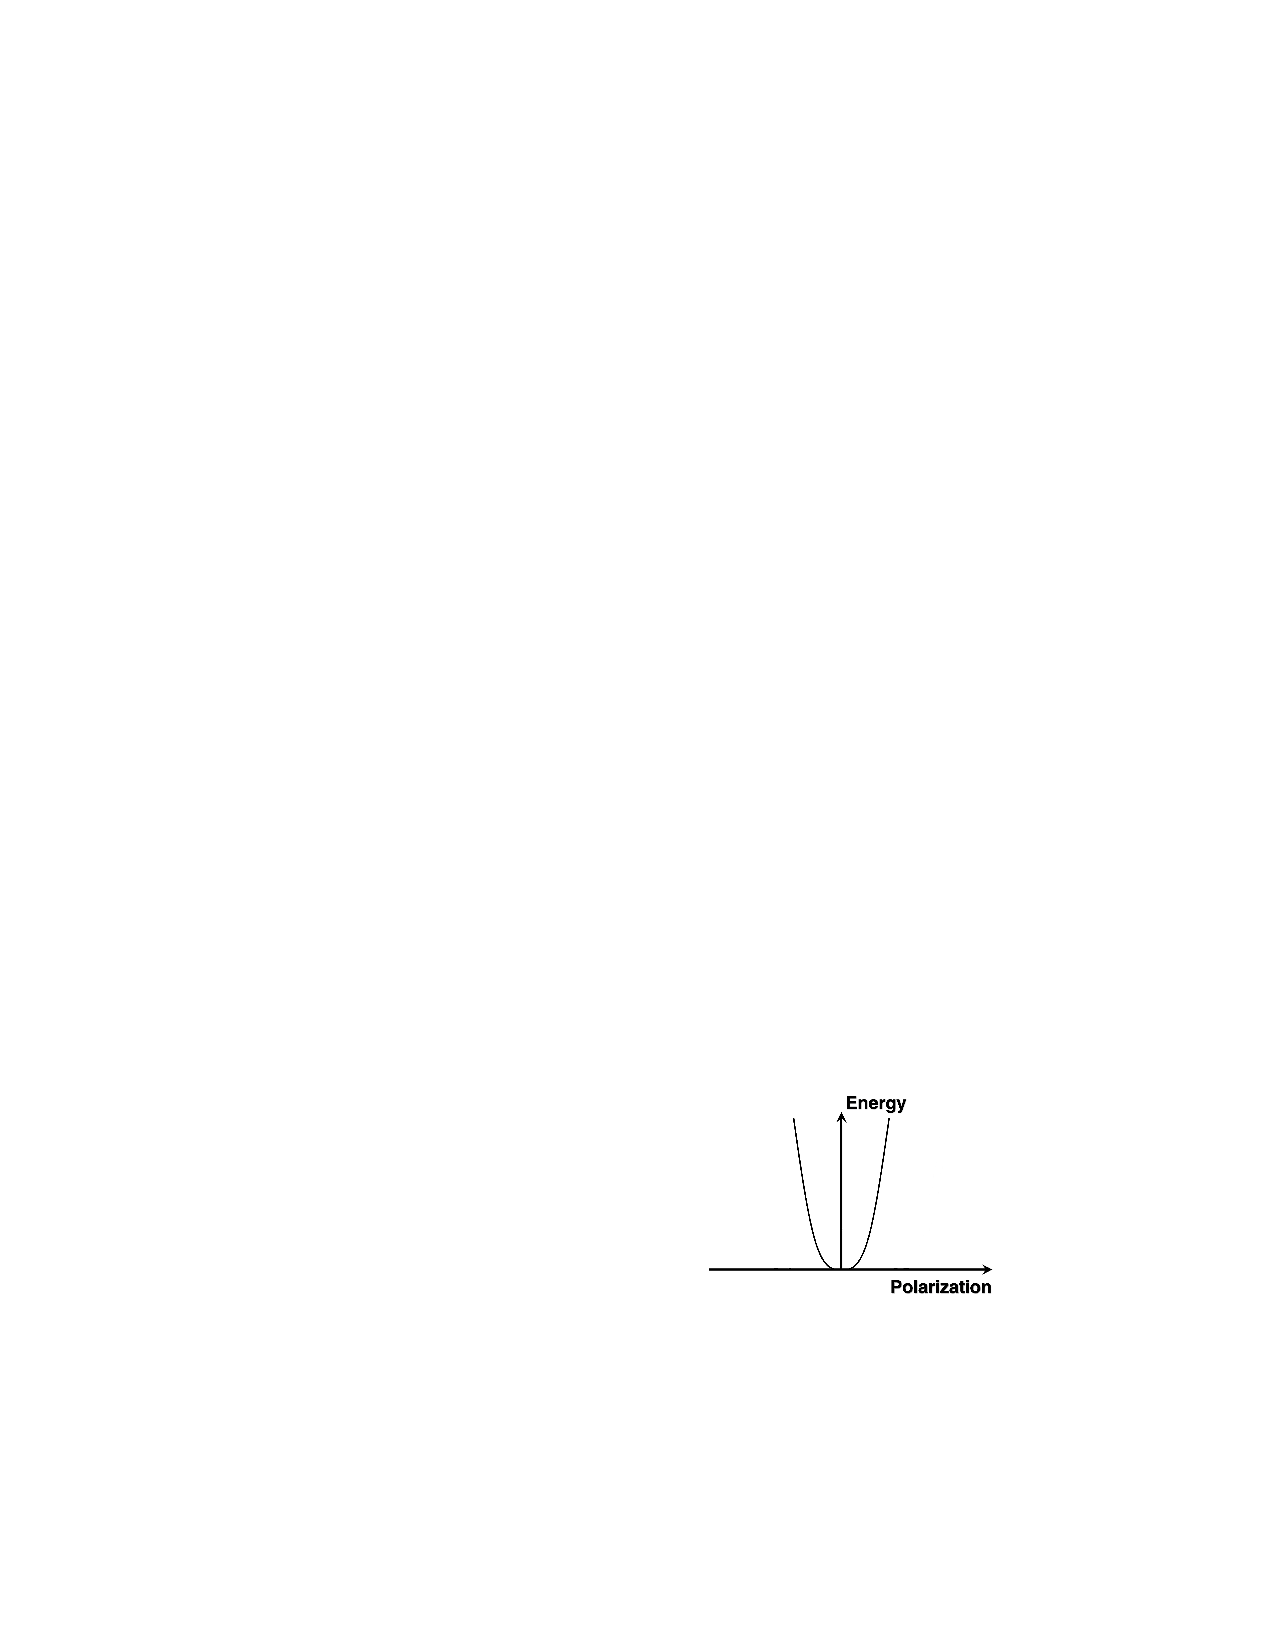
\includegraphics[width=0.45\linewidth]{./figures/materials/EvP-FE2}%
	} 	
   \subfloat[][Ferroelectric]{%
   	\label{fig:EvP-FE}%
	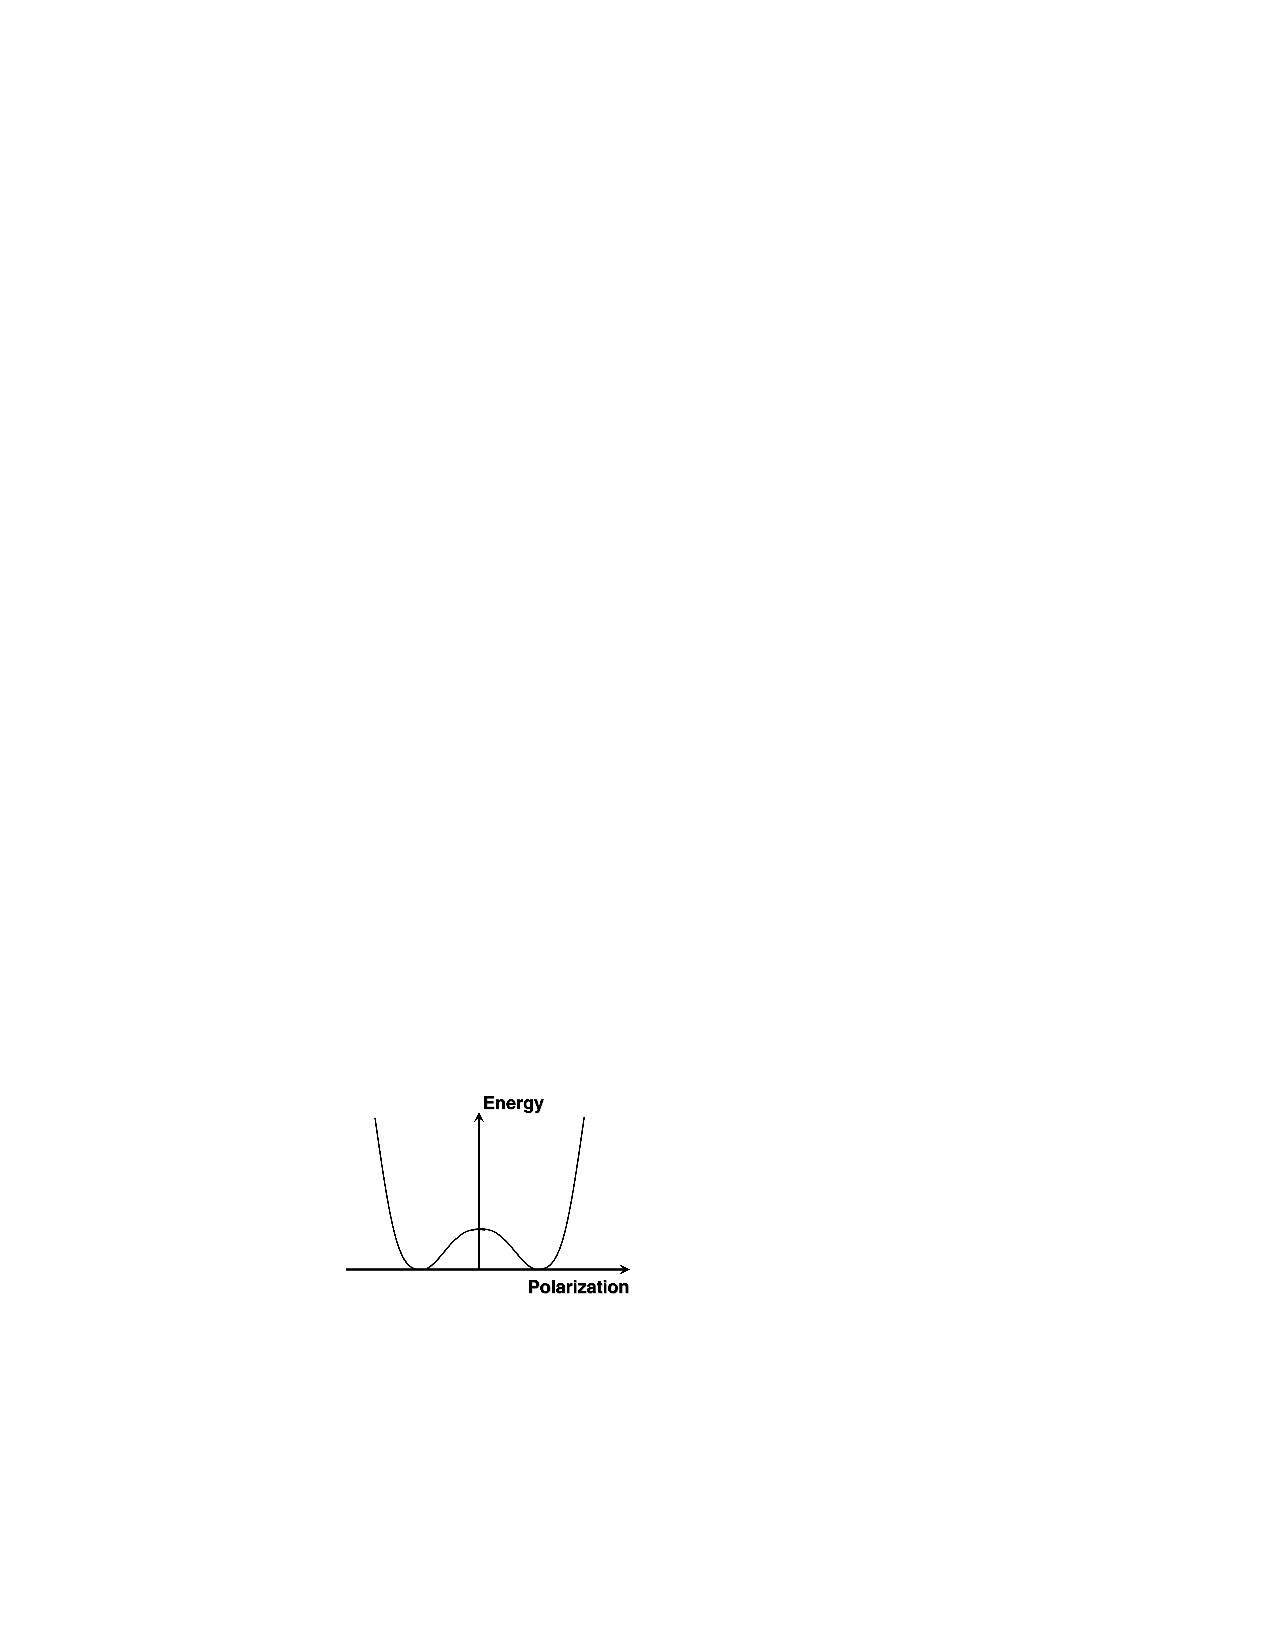
\includegraphics[width=0.45\linewidth]{./figures/materials/EvP-FE1}%
	} 	
   \caption[Energy vs. Polarization Plots for FE and PE Materials]%
   		{Example plots of the energy required to polarize a material. Ferroelectric materials (b) have %
		non-zero polarization at the energy minima. Above \Tc{} all ferroelectric materials transition %
		to a paraelectic phase (a). As temperature increases, the energy minima will approach one %
		another. These plots are generalized from equation~\vref{eq:landau-dev}.}
   \label{fig:EvP}
\end{figure}

\begin{figure}[tb]
   \centering
   \subfloat[][Paraelectric]{%
   	\label{fig:PvElec-PE}%
	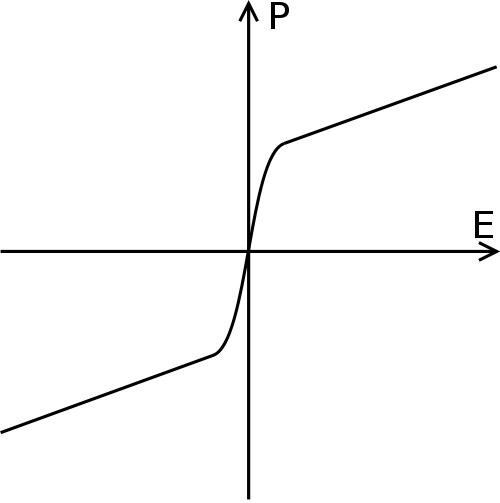
\includegraphics[width=0.4\linewidth]{./figures/materials/PvElec-PE}%
	} 
   \hspace{0.5cm}	
   \subfloat[][Ferroelectric]{%
   	\label{fig:PvElec-FE}%
	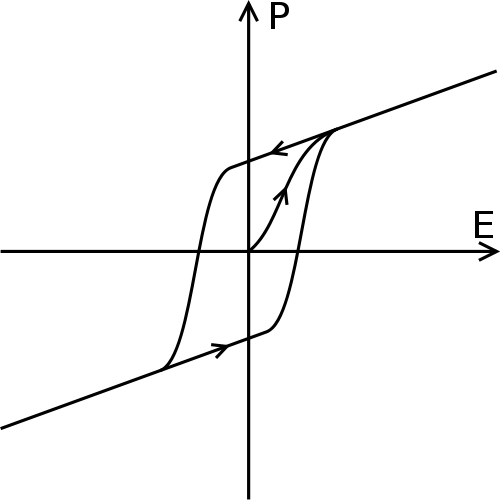
\includegraphics[width=0.4\linewidth]{./figures/materials/PvElec-FE}%
	} 	
   \caption[Polarization vs. Applied Field Plots for FE and PE Materials]%
   		{Example plots of the polarization as a function of applied field. (a) Paraelectric materials %
		have two regions of polarizability; at low E the polarization increases quickly with the field, %
		as E increases the rate of increase decreases. (b) Ferroelectric materials show similar %
		behavior, but additionally have hysteresis. This means that the films are switchable %
		between two states, but it is difficult to obtain zero polarization.\\%
		{\tiny Image Source: \url{http://en.wikipedia.org/wiki/Ferroelectricity} originally contributed by ``Bigly'' %
		under GNU-FDL.}}
   \label{fig:PvElec}
\end{figure}

%%%%%%%%%%%%%%%%%%%%%%%%%%%%%%%%%%%%%%%%%%%%%%%%%%%
%%%%%%%%%%%%%%%%%%%%%%%%%%%%%%%%%%%%%%%%%%%%%%%%%%%
%%%%%%%%%%%%%%%%%%%%%%%%%%%%%%%%%%%%%%%%%%%%%%%%%%%































\chapter{Synthesis Methods}
\label{chap:Synth}
\thispagestyle{empty}

%%%%%%%%%%%%%%%%%%%%%%%%%%%%%%%%%%%%%%%%%%%%%%%%%%%
%%%%%%%%%%%%%%%%%%%%%%%%%%%%%%%%%%%%%%%%%%%%%%%%%%%
%%%%%%%%%%%%%%%%%%%%%%%%%%%%%%%%%%%%%%%%%%%%%%%%%%%

Synthesis of perovskite oxides has been demonstrated using a wide range of techniques. These range from solution-based processing methods (sol-gel approach), to physical vapor methods (molecular beam epitaxy and pulsed laser deposition), and gas phase chemical methods (chemical vapor deposition and atomic layer deposition). This review will briefly discuss sol-gel and CVD methodology, but will focus in more depth on films deposited via ALD. 

%%%%%%%%%%%%%%%%%%%%%%%%%%%%%%%%%%%%%%%%%%%%%%%%%%%
%%%%%%%%%%%%%%%%%%%%%%%%%%%%%%%%%%%%%%%%%%%%%%%%%%%
%%%%%%%%%%%%%%%%%%%%%%%%%%%%%%%%%%%%%%%%%%%%%%%%%%%

\section{Sol-Gel Processing}
\label{sec:Synth-SolGel}

Sol-gel processing is a very commonly used technique for producing oxide films of a wide variety of types. It is rather straightforward in its method, but it is nonetheless a very powerful method for producing films with complex stoichiometries. Being a wet-chemical deposition technique, sol-gel has both advantages and disadvantages. It is a fairly low temperature deposition technique, but in order to obtain a fully dense and crystalline film a sintering and annealing step is often required. The solution-based nature of the chemistry lends itself to very close control of tolerances in the composition of the final film.\cite{brinker_sol-gel_1990,Yoldas_1979}

Sol-gel processing starts with the production of a colloidal solution containing all of the elemental precursors that are desired, in the precise ratios desired in the final film. Generally these precursors are metallic salts or metallic alkoxides, which are combined and then treated to undergo various co-reactions (hydrolysis, polycondensation, etc.) to form colloidal particles which become suspended in the solvent. By adjusting the pH and viscosity, the precursor sol can be converted into a gel which can be used to form a wide variety of structures such as fibers or powders.\cite{Fred_Al2O3_powders_1996,hanaor_solgel_tio2_2011}

For film synthesis, generally the sol is kept in a relatively low viscosity state and applied to a substrate via spin-coating techniques. Modulating the sol viscosity, rotor speed, and spinning time allows for relatively fine control over film thickness on planar structures, from the nanometer-scale to the micron-scale. The spun fluid is then heated to liberate any remaining solvent and catalyze the formation of the fully gelled structure. This low-density structure can subsequently be heat treated at a much higher temperature to sinter and anneal the film, providing a much denser sample as well as control over crystallinity and phase. This improves the mechanical stability of the film, due to the densification, and can improve material properties by controlling phase purity by the anneal step. \cite{brinker_sol-gel_1990,Fred_Al2O3_powders_1996,hanaor_solgel_tio2_2011,Yoldas_1979}

Sol-gel films are very commonly used to produce many different types of high-tech oxide films. \ce{PbZr_{x}Ti_{1-x}O3}\cite{Takashi_1994} is a very common ferroelectric material that is commonly produced in powder, film, and bulk forms via this technique. (Ba,Sr)Ti\ce{O3} is another.\cite{Tahan_1996}

Some of the disadvantages of sol-gel film deposition is the lack of truly precise control over the film thickness, its difficulty in evenly coating many types of 3-dimensional structures, as well as being somewhat difficult to integrate into conventional lithographic electronics processing.\cite{brinker_sol-gel_1990,Fred_Al2O3_powders_1996,hanaor_solgel_tio2_2011,Yoldas_1979} 

%%%%%%%%%%%%%%%%%%%%%%%%%%%%%%%%%%%%%%%%%%%%%%%%%%%
%%%%%%%%%%%%%%%%%%%%%%%%%%%%%%%%%%%%%%%%%%%%%%%%%%%
%%%%%%%%%%%%%%%%%%%%%%%%%%%%%%%%%%%%%%%%%%%%%%%%%%%

\section{Metallorganic Chemical Vapor Deposition}
\label{sec:Synth-MOCVD}

Metallorganic chemical vapor deposition (MOCVD) is a commonly used technique for depositing many different types of thin film materials. It is especially common for MOCVD to be used to deposit semiconductor films (a-Si, Ge, III-V, II-VI, etc.); these films can also be doped to varying degrees with high precision.\cite{Malshe_1999,Matsumara_1998,Muralt_2000}

A CVD process begins with the introduction of reactant vapors into the reactant chamber. The chamber is heated to a temperature sufficient to cause pyrolysis --- thermal cracking --- of the reactant. This liberates the desirable element, the metallic portion of the compound, allowing it to adsorb to the substrate. Over time a thin film is deposited. Films of multiple elements are formed by introducing two different reactants into the chamber simultaneously; the same principle works for dopants, but at a much lower concentration.\cite{Malshe_1999,Matsumara_1998,Muralt_2000} 

One advantage of CVD, partly due to the high deposition temperatures involved, is the ability to have the film deposit epitaxially to the substrate. This allows for the creation of perfect, or nearly perfect depending on the lattice matching between film and substrate, interfaces. This is very desirable for a great number of applications, primarily in the semiconductor field.\cite{Malshe_1999,Matsumara_1998,Muralt_2000} 

%%%%%%%%%%%%%%%%%%%%%%%%%%%%%%%%%%%%%%%%%%%%%%%%%%%
%%%%%%%%%%%%%%%%%%%%%%%%%%%%%%%%%%%%%%%%%%%%%%%%%%%
%%%%%%%%%%%%%%%%%%%%%%%%%%%%%%%%%%%%%%%%%%%%%%%%%%%

\section{Atomic Layer Deposition}
\label{sec:Synth-ALD}
	
Atomic Layer Deposition (ALD) is a modification on standard CVD processes, with a few major differences. The defining aspect of an ALD process is the separation of the overall reaction into two steps: first the precursor is allowed to react with the substrate surface (see reaction~R~\ref{chem:TMA1}), excess reactant is purged from the chamber and an oxidizer is introduced to complete the reaction (see reaction~R~\ref{chem:TMA2}).\cite{ALD-Handbook} These reactions show a very simple ALD reaction between trimethylaluminum (TMA, \ce{Al(CH3)3}) and water. 

\begin{reactions}
	Al(CH3)3 + M-OH_{surf} &-> M-O-Al(CH3)2_{\,surf} + CH4 \label{chem:TMA1}%
		\AddRxnDesc{TMA: Precursor-Surface Site Reaction}%
		\\
	M-O-Al(CH3)2_{\,surf} + 2H2O &-> M-O-Al(OH)2_{\,surf} + 2CH4 \label{chem:TMA2}%
		\AddRxnDesc{TMA: Ligand Oxidation \& Site Regeneration}
\end{reactions}


In this example, it is seen that the first stage allows the TMA to react with the hydrated substrate surface to form part of a layer of alumina (\ce{Al2O3}), liberating a molecule of methane as a byproduct. In the next step, the remaining ligands are stripped away from the bound TMA molecule and replacing them with hydroxyl groups. This returns the system to the initial state --- where the surface is presenting sites available to react with more TMA --- and the cycle is completed. A graphical example of this process can be found in figure~\ref{fig:TMA-illustration}.


\begin{figure}[tbp]
   \centering
   \subfloat[][Precursor injection]{%
%   	\label{fig:Q50-image}%
	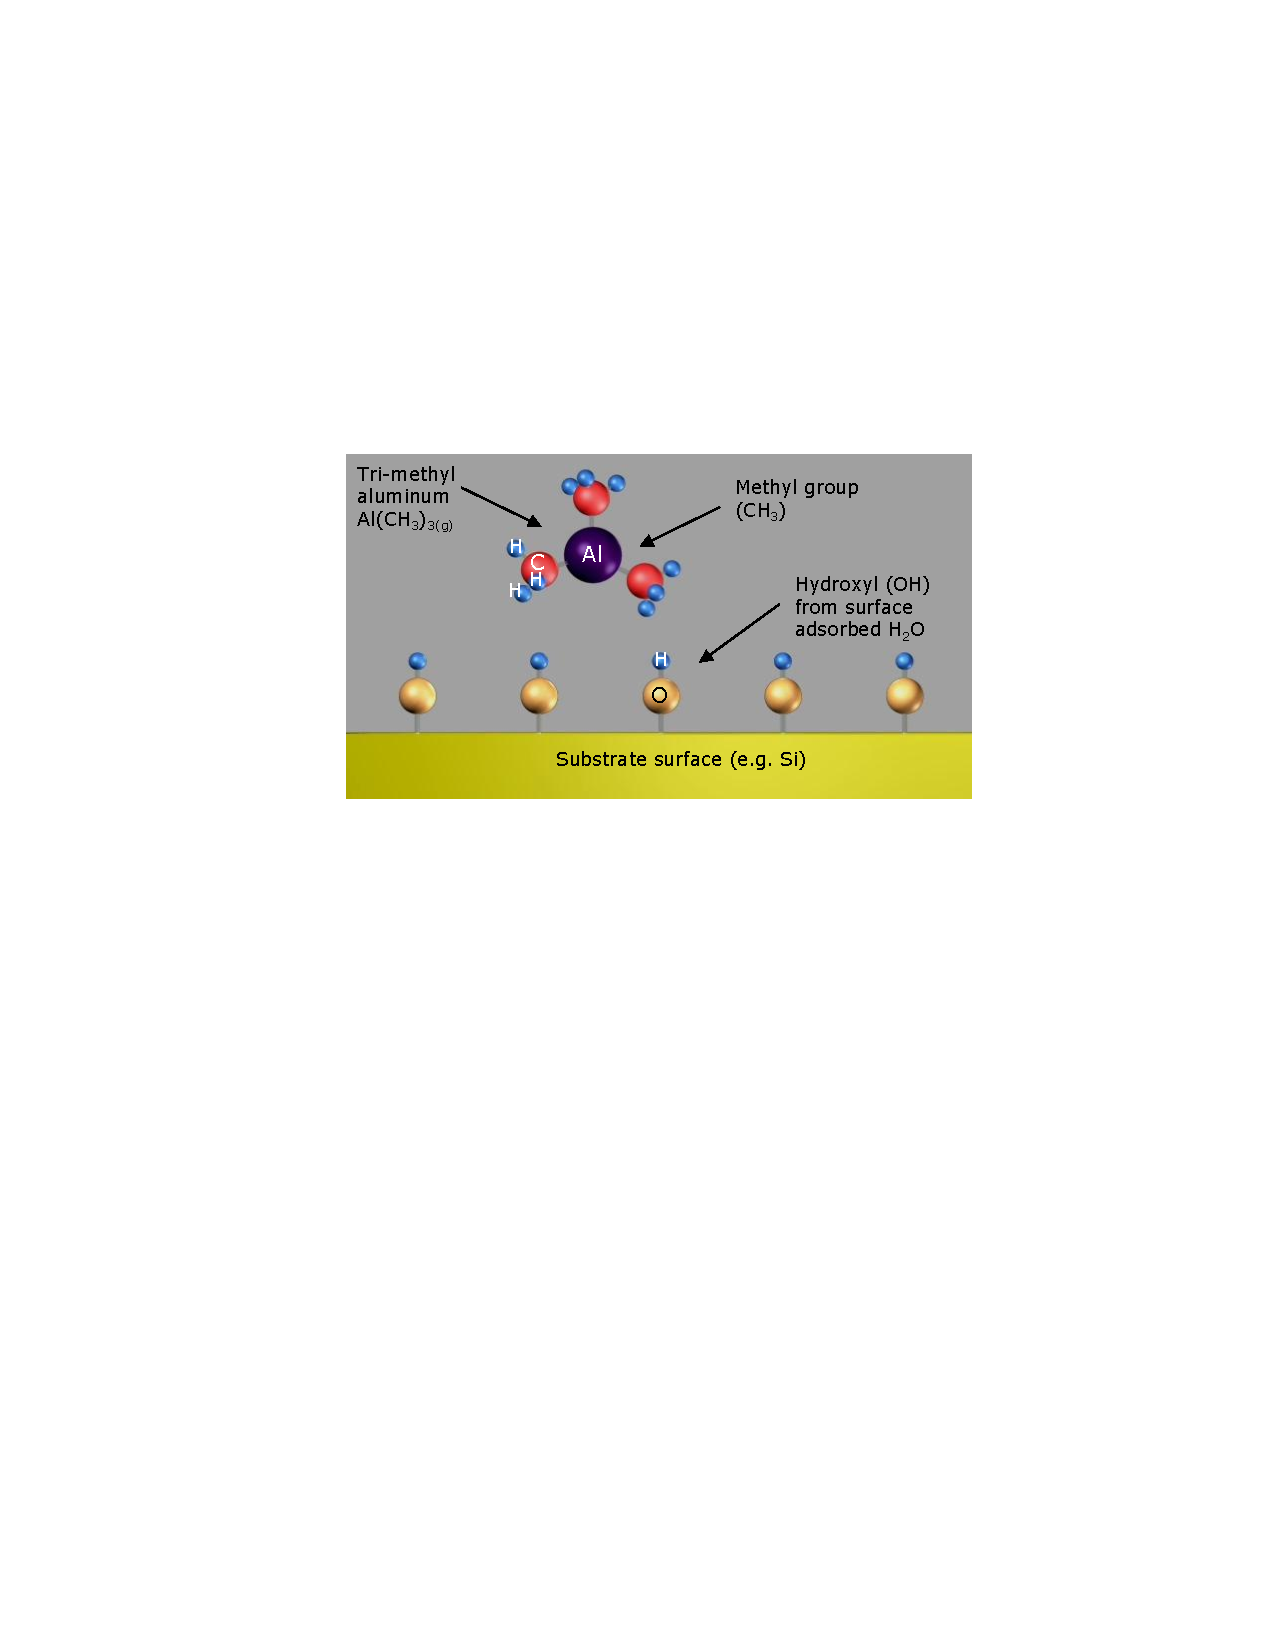
\includegraphics[width=0.45\linewidth]{./figures/synthesis/TMA1}%
	} 
	\hspace{6pt}
  \subfloat[][Precursor reaction]{%
%   	\label{fig:Q50-image}%
	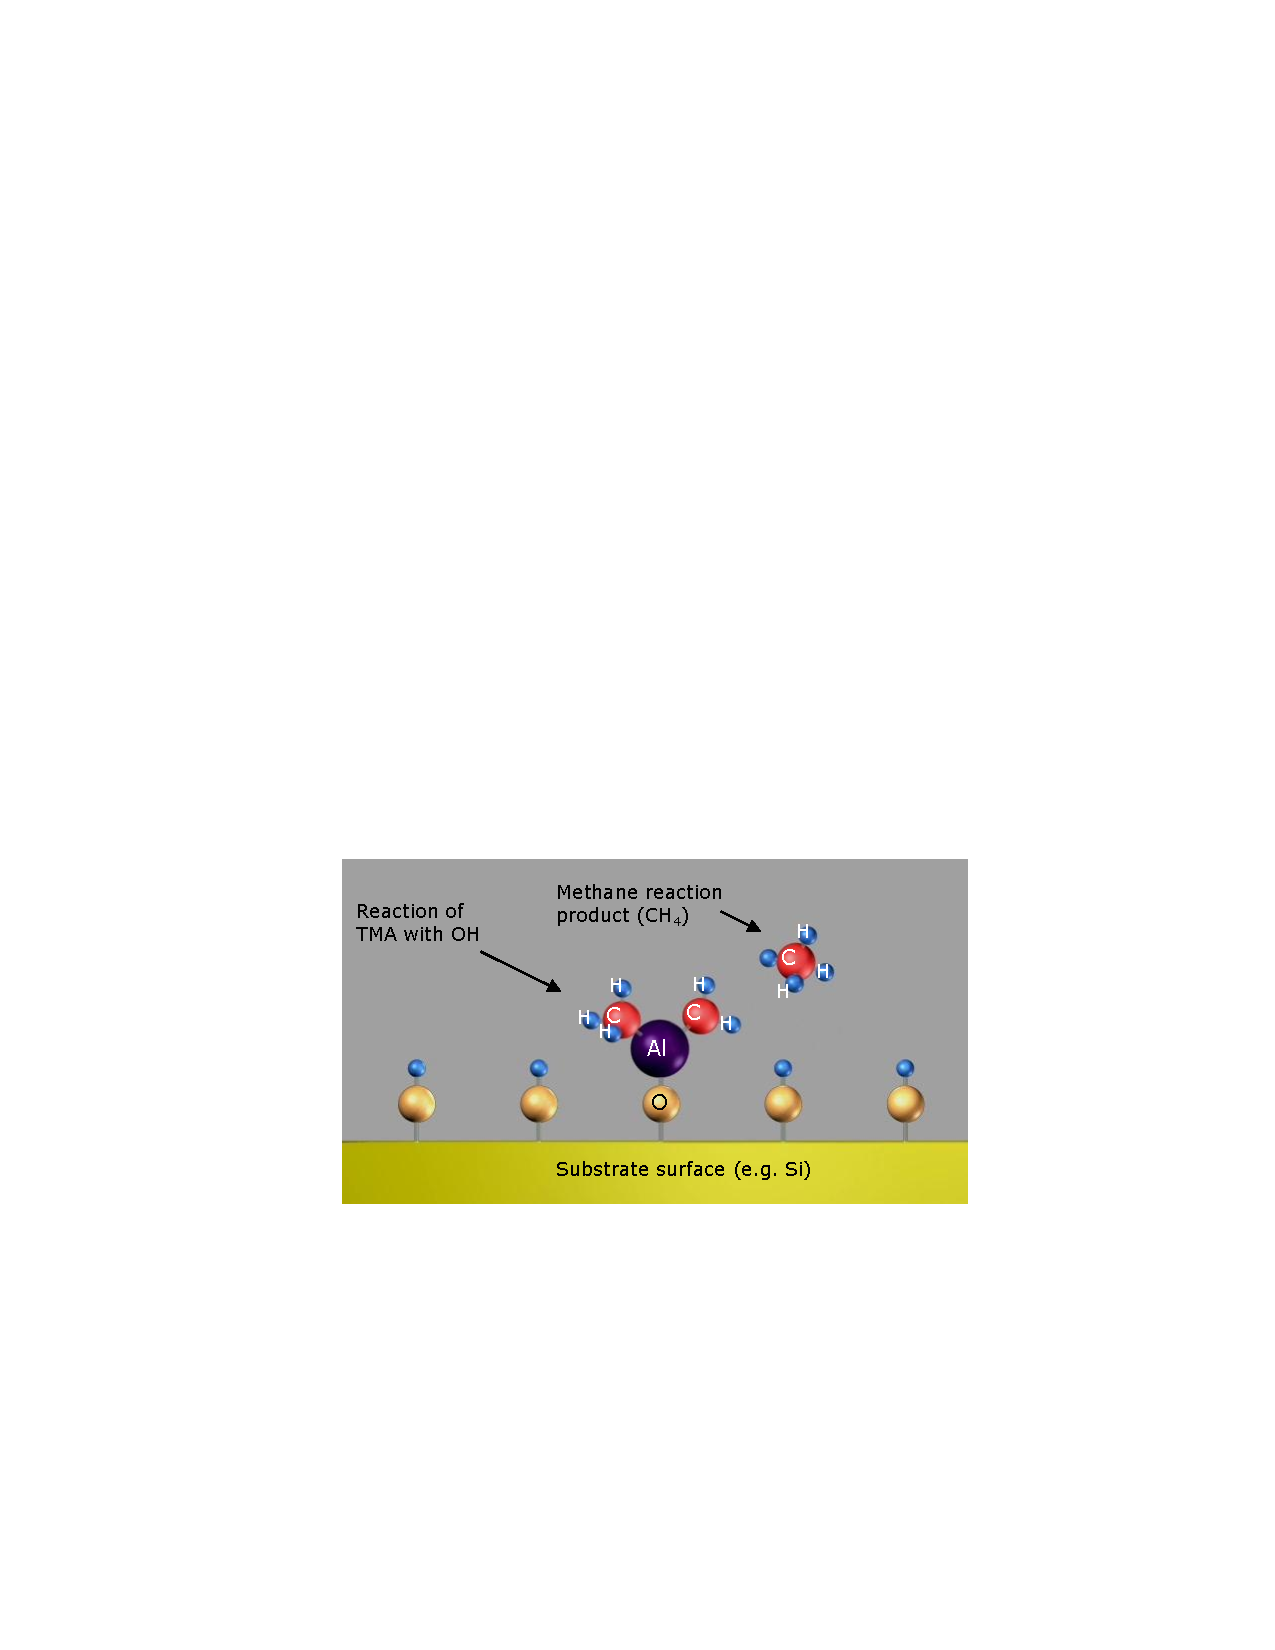
\includegraphics[width=0.45\linewidth]{./figures/synthesis/TMA2}%
	} \\
  \subfloat[][Reactor Purging]{%
%   	\label{fig:Q50-image}%
	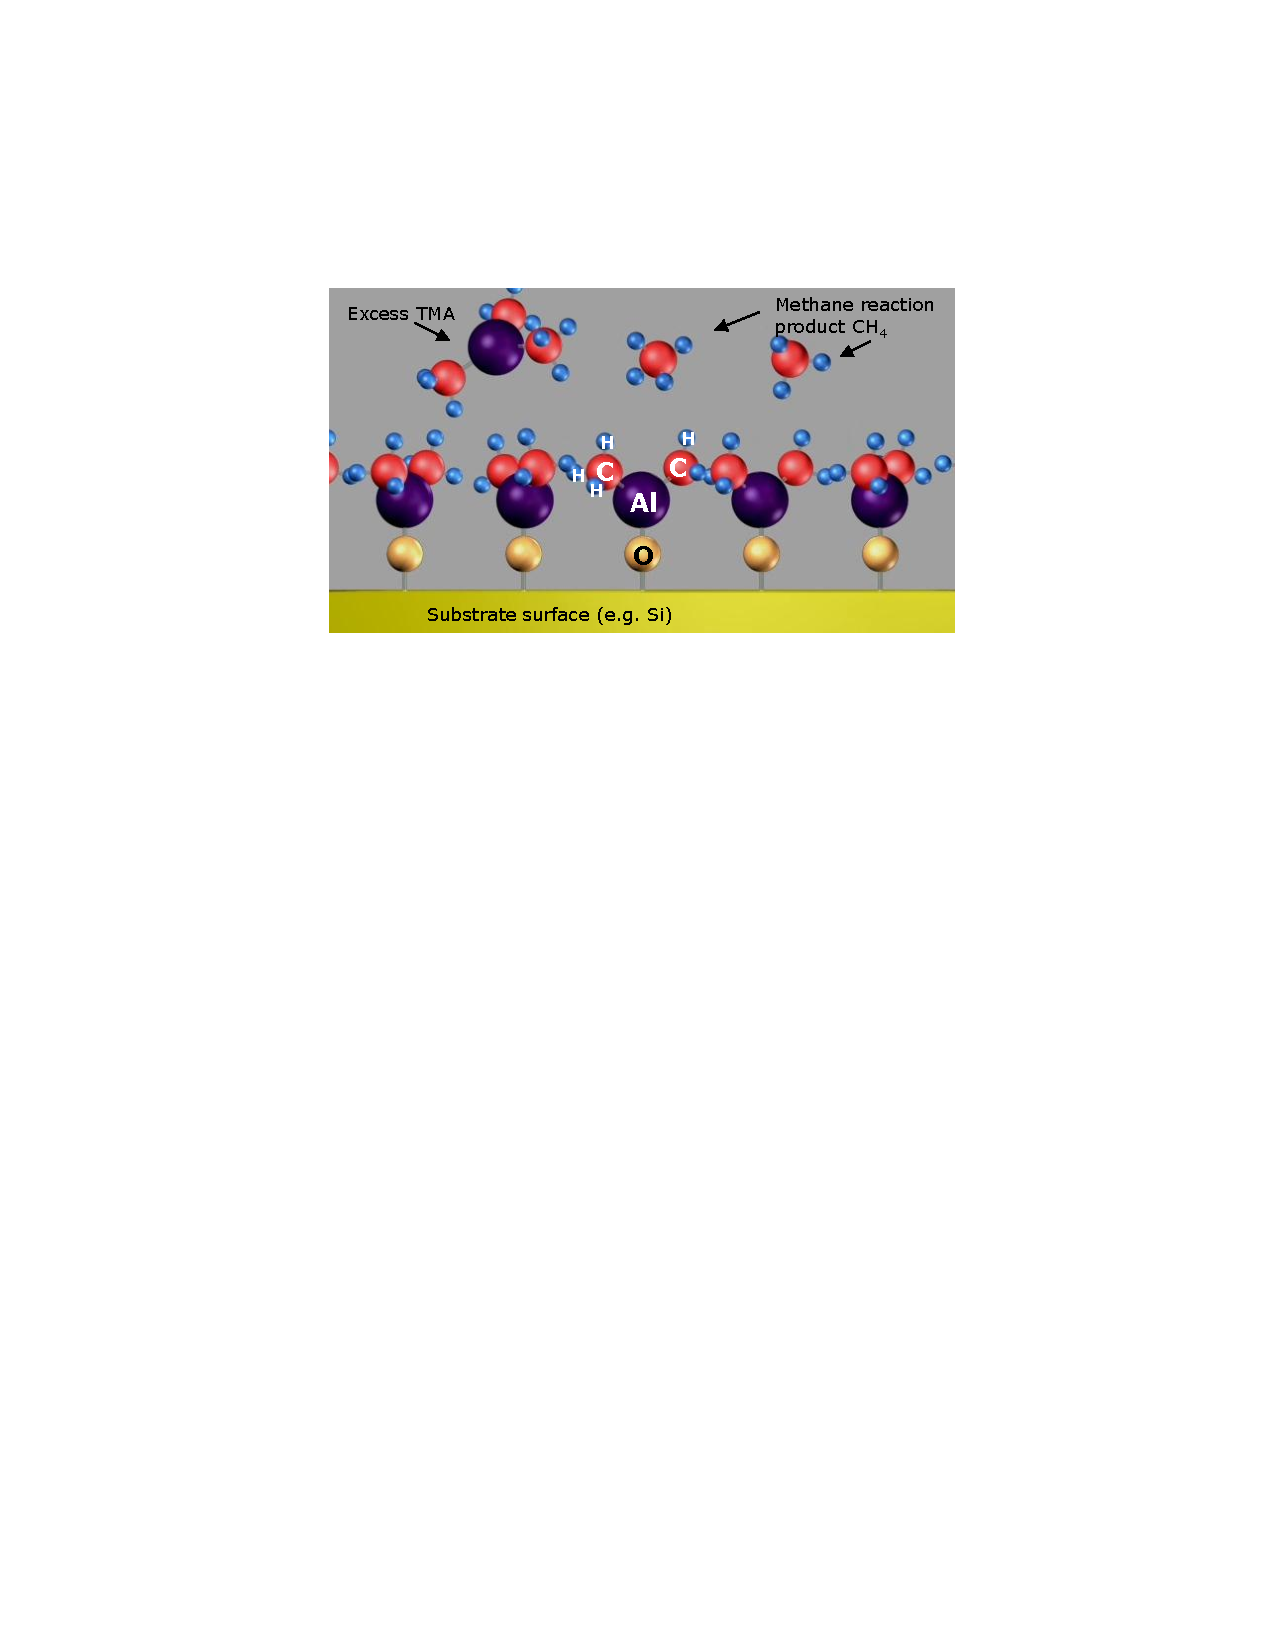
\includegraphics[width=0.45\linewidth]{./figures/synthesis/TMA3}%
	}  
	\hspace{6pt}	
  \subfloat[][Oxidant Injection]{%
%   	\label{fig:Q2000-image}%
	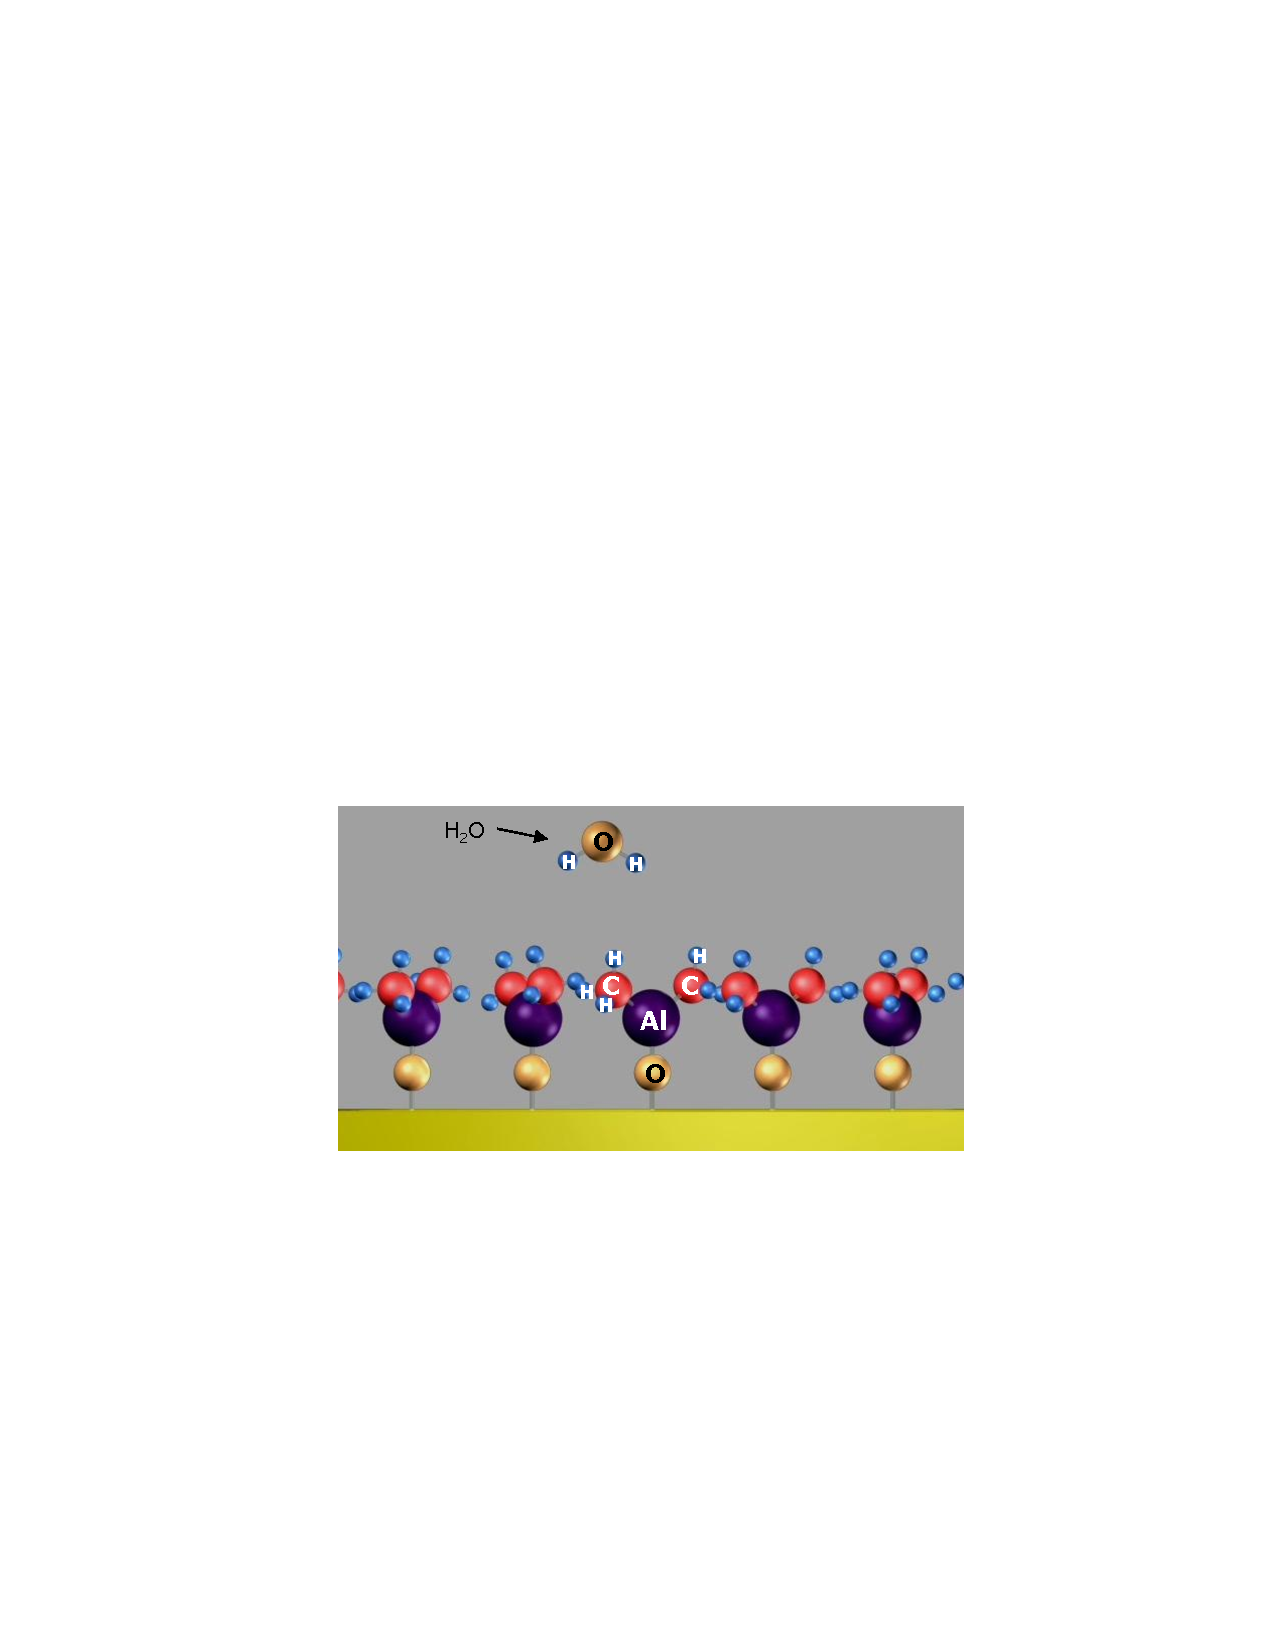
\includegraphics[width=0.45\linewidth]{./figures/synthesis/TMA4}%
	} \\
  \subfloat[][Oxidation Reaction (Ligand Exchange)]{%
%   	\label{fig:Q2000-image}%
	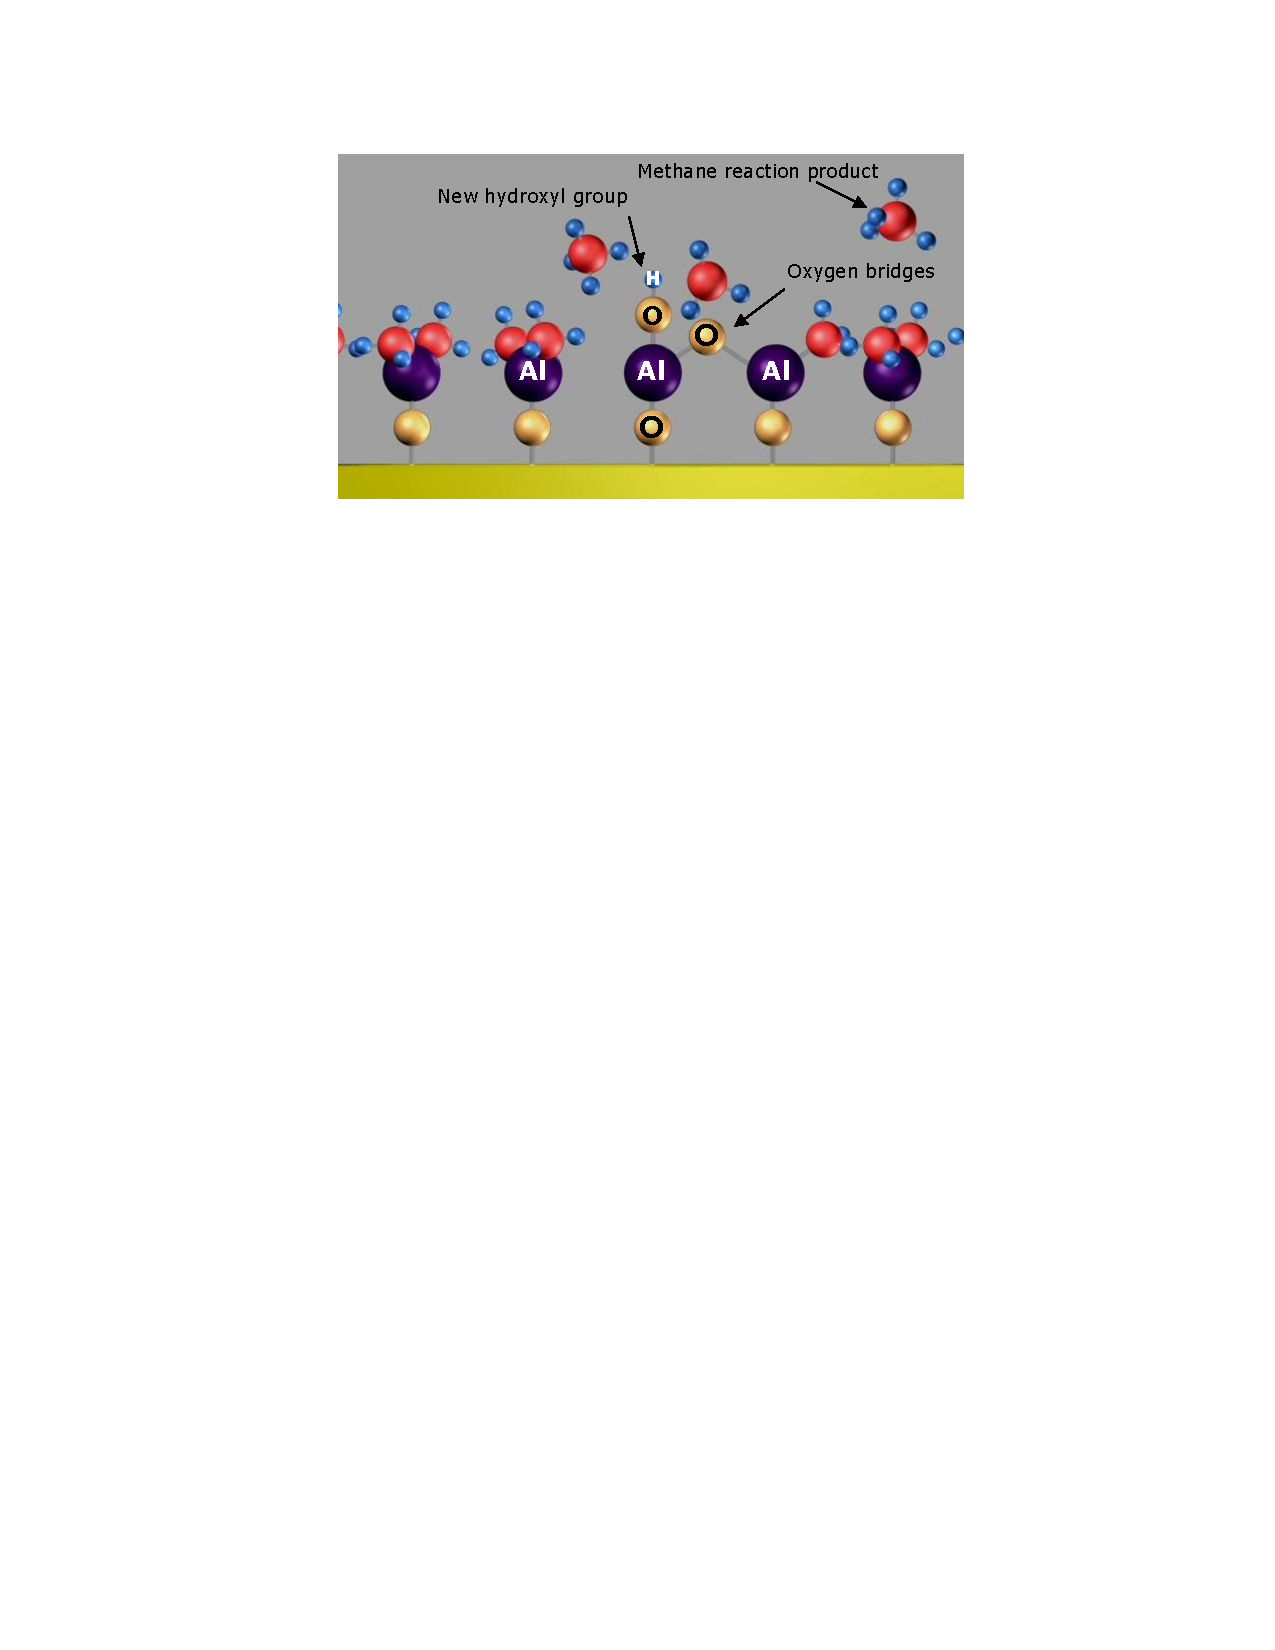
\includegraphics[width=0.45\linewidth]{./figures/synthesis/TMA5}%
	} 
	\hspace{6pt} 
  \subfloat[][Completed Cycle, Regenerated Surface]{%
%   	\label{fig:Q2000-image}%
	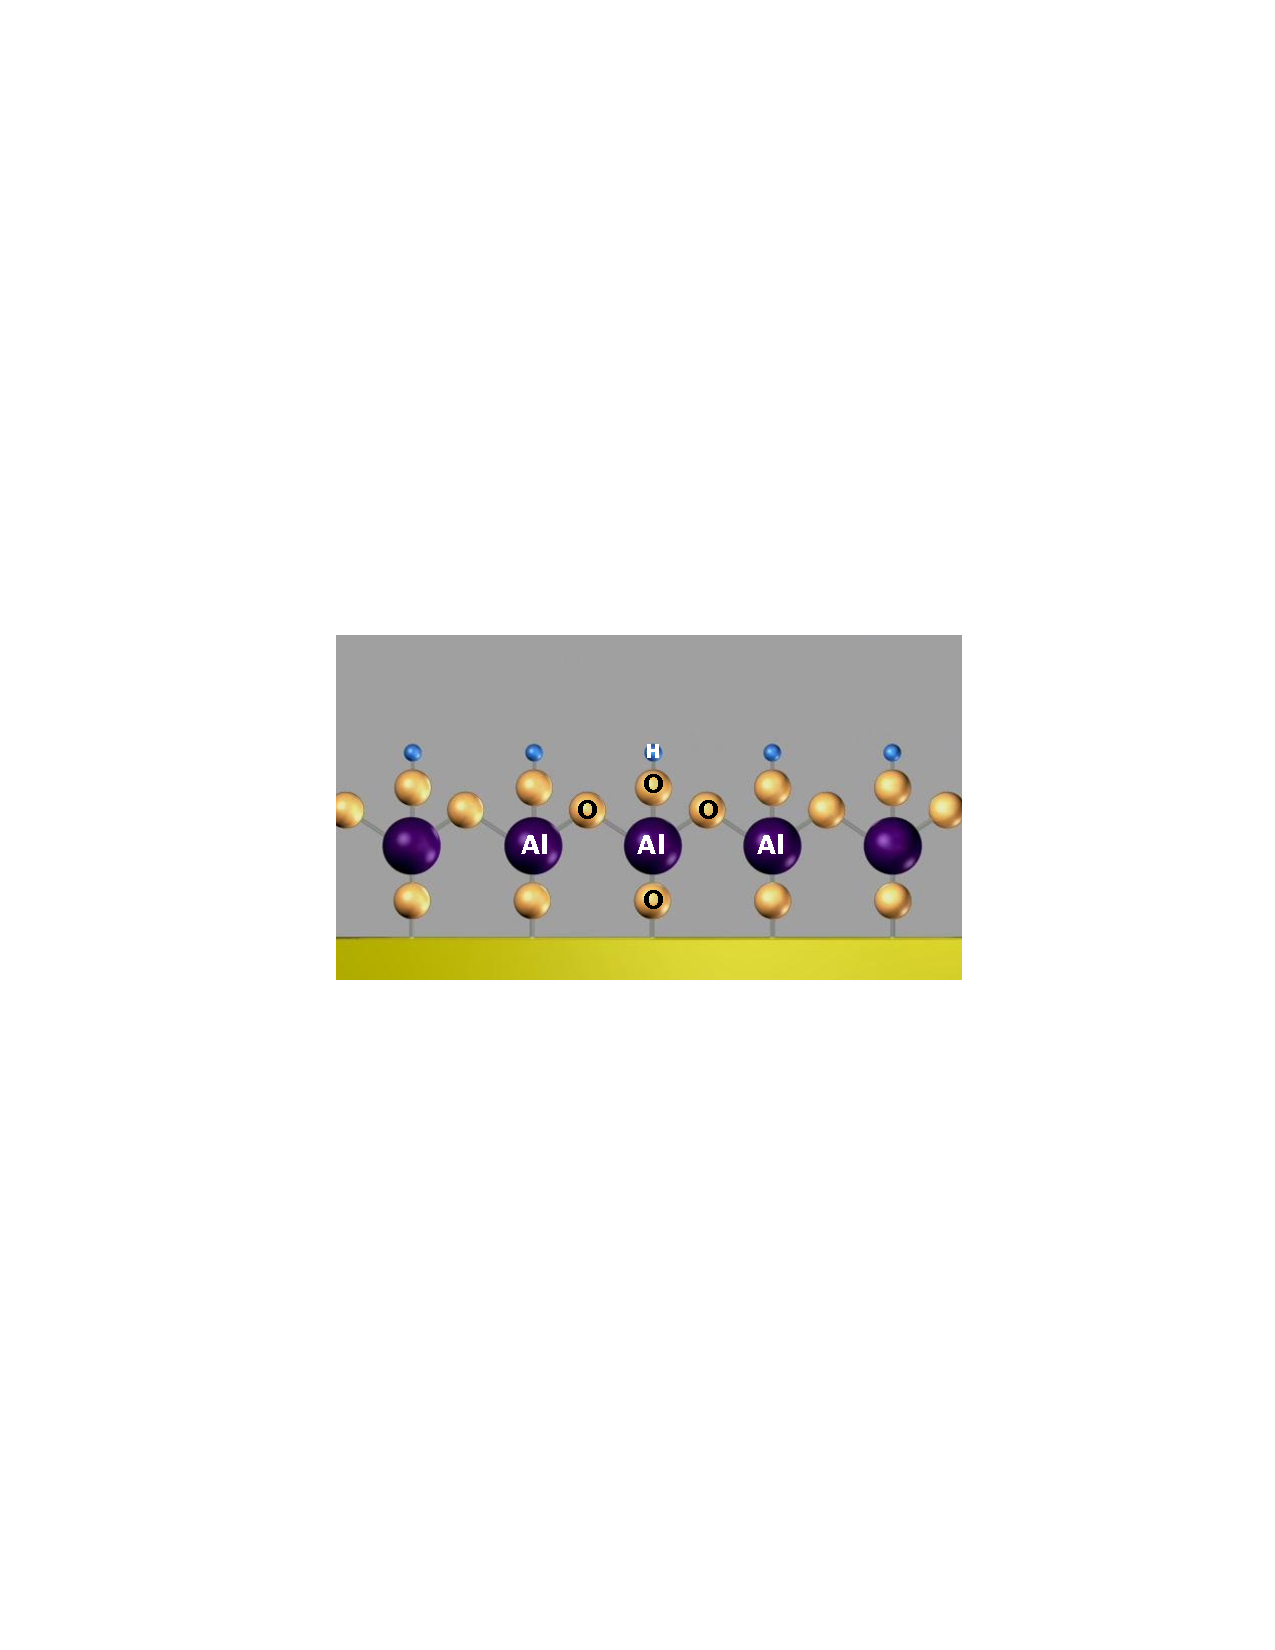
\includegraphics[width=0.45\linewidth]{./figures/synthesis/TMA6}%
	} 	
   \caption[Illustration of Example ALD Cycle]%
   		{Example schematic of the process of an ALD deposition cycle. This example\\%
		illustrates the reaction of TMA and water to form alumina (\ce{Al2O3}). \\%
		{\tiny Graphics reprinted with permission of Cambridge NanoTech, Inc.}\cite{CNT-web}}
   \label{fig:TMA-illustration}
\end{figure}

Having only surface reactions be permitted, as opposed to CVD where gas-phase interactions dominate, affords ALD a number of unique characteristics. One of these is the concept of the ``self-limiting'' growth mode.\cite{ALD-Handbook} This behavior arises from the limited number of available reaction sites; when all of these have either been reacted with or made unavailable by a blocking mechanism such as stearic hindrance from other local chemisorbed precursor the reaction can no longer proceed. At this point, additional available precursor is not going to be utilized, and instead will be removed and treated as waste material. The system is then evacuated, and a inert purge gas such as dry nitrogen or argon is flowed through the reactor. The purge gas serves both to push any remaining gases out of the reactor as well as to help desorb physisorbed species from the surface. The system would then again be evacuated, and the oxidant introduced and then pumped away to complete the cycle. Because of the self-limiting behavior of the reactants it is possible, in fact preferable, to utilize reactants that have highly energetic reactions with their corresponding surface site. For ALD, having fast and energetic reactions allows for rapid completion of the half-cycle, which allows for faster cycle times and thus higher throughputs. In CVD such energetic reactions are very difficult to control, and instead precursors that have only mild reactions --- with a Gibbs free energy exchange as close to zero as possible while remaining negative --- with each other are preferred. These require more effort to develop and require that the process be carefully controlled, as the reactions often can either easily extinguish themselves or rapidly accelerate in different conditions.\cite{ALD-Handbook}

In the implementation of most ALD systems, the purge gas is also used as a carrier gas for the precursors. Thus a constant flow of gas is passed through the system, instead of having it occasionally fully evacuated, and the precursor is able to be delivered from its source to the reactor more effectively. For some precursor compounds, in particular those with a low vapor pressure, having carrier-assisted transportation can greatly improve the behavior of the system.\cite{ALD-Handbook} 

Because of the self-limiting behavior, each deposition cycle is limited to a theoretical maximum of one monolayer of material (in practice a much lower coverage per cycle is attained), which is far less than a unit cell.\cite{ALD-Handbook} Generally per cycle growth rates range between 0.03--1.5 \AA{}, with the rate being nearly invariable during most of the deposition. This gives the second defining characteristic of ALD: very high (\AA\ level) thickness resolution. The downside of this aspect is that growths are generally much slower than other types of depositions; ALD is generally slower by an order of magnitude or more than a similar CVD process, as an example. This has proved invaluable in many processes where high precision is critical, such as electronics manufacturing. Intel, for example, uses ALD to deposit extremely precise layer thicknesses of a high-$\kappa$ dielectric (such as hafnia, \ce{HfO2}) for use as the gate oxide in transistors.\cite{toriumi_application_2008,chen_atomic_2007}

There are a wide range of binary oxides for which ALD processes have been developed. A deposition for alumina (\ce{Al2O3}, one of the first ALD materials developed, was discussed briefly above and the method is is common use.\cite{lee_al2o3_2003,puurunen_surface_2005} High-$k$ gate oxides such as hafnia and zirconia (\ce{ZrO2}), along with some of their nitrides and silicides, are under intense research to develop industrial processes for their use in integrated circuitry.\cite{toriumi_application_2008,chen_atomic_2007} Other transition metal oxides, such as titania (\ce{TiO2}) and iron oxide (\ce{Fe2O3}), have also had ALD deposition processes developed for their deposition. \cite{lim_atomic_2003,scheffe_atomic_2009}

The methods described above will produce a layer of a binary oxide material (\ce{AO_{x}}); if more complex materials are desired the method must be changed. The basic principles remain the same; one would perform the procedure for depositing a cycle of a binary oxide and then change the precursor and deposit another cycle of a different oxide material. For example, if one wished to deposit \PTO{}, one would begin by depositing a layer of \ce{TiO2} and then depositing a layer of lead oxide (\ce{PbO}). Repeating this set of cycles --- a super-cycle --- would eventually form an ternary oxide film. 

However, deposition of \ce{ABO3} oxides is not this simple in practice. In many cases, running each oxide cycle in a 1:1 ratio will deposit a non-stoichiometric material. This makes it necessary to modify the method to deposit more of one type of oxide than the other. For example, if a material is Ti-rich the super-cycle ratio would be modified to increase the number of lead oxide cycles as compared to the titania cycles. Careful tuning of the deposition conditions, which include a variety of different factors, is required to obtain a desired and consistent film stoichiometry. 

In addition to lead titanate, there are other ternary oxide systems that are being investigated. Examples of which are bismuth ferrite (\ce{BiFeO3}) or barium strontium titanate (\ce{(Ba\,Sr)TiO3}).\cite{chu_nanoscale_2009}

ALD reactions are rather sensitive to a number of factors, such as temperature. The temperature must be high enough that the reactants have sufficient energy to drive the surface reaction but not so high as to allow undesirable reactions to activate (e.g. precursor cracking or surface material desorption). Precursor selection is also very important, for similar reasons. The precursors must also be incapable of reacting with themselves, to allow the self-limiting mechanism to work properly.\cite{ALD-Handbook}


%
%\begin{subreactions}
%	\label{chem:2TMA}
%	\begin{reactions}
%		Al(CH3)3 + M-OH_{surf} &-> M-O-Al(CH3)2_{\,surf} + CH4 \label{chem:2TMA1} \\
%		M-O-Al(CH3)2_{\,surf} + 2H2O &-> M-O-Al(OH)2_{\,surf} + 2CH4 \label{chem:2TMA2}
%	\end{reactions}
%\end{subreactions}
%
%\begin{subreactions}
%\newcommand*{\thesubequation}{(\reactiontag.\alph{equation})}
%\label{chem:TMA}
%\begin{align}
%	\cee{Al(CH3)3 + M-OH_{surface} &-> M-O-Al(CH3)2_{\ surf} + CH4}%
%		\label{chem:TMA1}
%		\\
%	\cee{M-O-Al(CH3)2_{\ surf} + 2H2O &-> M-O-Al(OH)2_{\ surf} + 2CH4}%
%		\label{chem:TMA2}
%\end{align}
%\end{subreactions}



\lipsum








\chapter{Thin Film Growth}
\label{ch:SampFab}
\thispagestyle{empty}


%%%%%%%%%%%%%%%%%%%%%%%%%%%%%%%%%%%%%%%%%%%%%%%%%%%%%%%%%%
%%%%%%%%%%%%%%%%%%%%%%%%%%%%%%%%%%%%%%%%%%%%%%%%%%%%%%%%%%
%%%%%%%%%%%%%%%%%%%%%%%%%%%%%%%%%%%%%%%%%%%%%%%%%%%%%%%%%%

\section{Precursor Selection}
\label{sec:SampFab-Precursors}

\lipsum

%%%%%%%%%%%%%%%
\subsection{Titanium Source}

The source of titanium that was used was titanium(IV) isopropoxide (\TiOiPr{}, \ce{Ti(OCH(CH3)2)4}). This compound is very commonly used in ALD literature.\cite{cianci_atomic_2012,tallarida_growth_2011,lehnert_plasma_2012,cleveland_role_2012,kubrin_stacking_2012,lee_emph-situ_2012} It is a liquid precursor with a high vapor pressure and reacts easily with most oxidizers; the most commonly used oxidant for this reaction is water vapor, similar to the TMA-\ce{H2O} reaction (see Section~\vref{sec:Synth-ALD}). 

%%%%%%%%%%%%%%%
\subsection{Lead Source}

One of the primary tasks of this project was to identify viable ALD precursors for the deposition of lead into the thin films. Potential candidates needed to meet a few stipulations. First, it needed to have chemical and thermal properties compatible with the ALD reactor. It was also desired that previous studies had used it in other ALD processes. Finally, it was important that the compound was available in quantity from chemical suppliers. 

To this end, there were four potential candidates that were investigated which were identified from previous literature reports: tetraphenyllead (\ce{Ph4Pb})\cite{harjuoja_2006}, lead(II) bis(2,2,6,6-tetramethyl-3,5-heptanedionato) (\ce{Pb(TMHD)2})\cite{watanabe_growth_2007}, lead(II) hexafluoroacetylacetonate (\ce{Pb(HFAc)2})\cite{Igumenov_1998}, and lead bis(3-N,N-dimethyl-2-methyl-2- propanoxide) \\\noindent(Pb(DMAMP)$_{2}$).\cite{Hwang_2007}

\ce{Ph4Pb} was one of the commonly used compounds in both ALD and MOCVD references, but it was found to have insufficient volatility for use in the ALD (up to its maximum evaporation temperature of 200\degC{})\cite{harjuoja_2006} and was thus discarded as a candidate. \TMHD{} was another commonly referenced precursor\cite{watanabe_growth_2007}, as was \HFAc{}.\cite{Igumenov_1998} \ce{Pb(DMAMP)2} was seemingly a viable choice, with a very high vapor pressure at low temperatures,\cite{Hwang_2007} but it was not readily available from chemical suppliers and was very costly to purchase which kept it from being considered further. 

Thus, the two compounds \HFAc{} and \TMHD{} were investigated in detail as potential candidates for the lead precursor in the ALD deposition of \PTO{}. Samples of both precursors were obtained from Strem Chemicals, Inc.\cite{strem_inc} and were analyzed to determine which would be most viable. Tests included thermogravimetric analysis (TGA), differential scanning calorimetry (DSC), as well as test depositions of ALD films. 

%%%%%%%%%%%%%%%

\subsection{Oxidizer}

Three potential oxidants were considered; these included water, oxygen, and an ozone/oxygen mix. The choice of oxidant depends heavily on the reactivity with the potential precursors. 

The choice of titanium(IV) isopropoxide as the titanium source allows for any of the three selected oxidizers to be used. A hydrolysis reaction will occur when exposed to water vapor; in the case of oxygen or ozone the ligands will be consumed via a combustion reaction.\cite{ALD-Handbook,Leskela_2002,lim_atomic_2003}

Based on literature reports, the two lead precursors under investigation do not undergo hydrolysis when exposed to water, and as such require the use of the combustion pathway. In addition, through the deposition of test films, it was found that the reaction proceeded more completely when the \ce{O3}/\ce{O2} mixture was used. For simplicity of the process, the \ce{O3}/\ce{O2} mix was used for both half-reactions.\cite{KeunKim2005103}


%%%%%%%%%%%%%%%

\subsection{Proposed Reaction Pathway}

The reaction pathway seen in figure~\vref{fig:PTO-pathway} is a simplified graphical visualization (in the same character as that seen in figure~\vref{fig:TMA-illustration} for TMA) of ALD deposition using \TMHD{} and \TiOiPr{} and an \ce{O2}/\ce{O3} mixture as an oxidant.  

The chemical reactions seen below (in reactions R~\ref{rxn:PTO-Pb1}--\ref{rxn:PTO-Ti2}) also propose a preliminary mechanism for the chemisorption and oxidation/combustion of the precursors to deposit the film. As the materials involved are rather large, in particular \TMHD{}, the molecules have a large stearic hindrance once the chemisorption begins. This impedes the deposition of more than a small fraction of a monolayer per cycle, with lead depositing more slowly than titanium. Therefore, it is likely to have to apply the \TMHD{} half-reaction more often than the \TiOiPr{} reaction when depositing the material. 

{\footnotesize \addtocounter{reaction}{-2} \onehalfspacing
\begin{reactions}
	Pb(TMHD)2 + M-OH_{surf} &-> M-O-Pb(TMHD)_{\,surf} + H(TMHD) \label{rxn:PTO-Pb1}%
%		\AddRxnDesc{PTO: Pb(TMHD) chemisorption}%
		\\
	M-O-Pb(TMHD)_{\,surf} + xO2 + xO3 &-> M-O-Pb(OH)3_{\,surf} + yCO2 + zH2O \label{rxn:PTO-Pb2}%
%		\AddRxnDesc{PTO: Pb(TMHD) oxidation}
		\\
	Ti(OCH(CH3)2)4 + M-OH_{surf} &-> M-O-Ti(OCH(CH3)2)3_{\,surf} + HOC3H7 \label{rxn:PTO-Ti1}%
%		\AddRxnDesc{PTO: Pb(TMHD) chemisorption}%
		\\
	M-O-Ti(OCH(CH3)2)3_{\,surf} + xO2 + xO3 &-> M-O-Ti(OH)3_{\,surf} + yCO2 + zH2O \label{rxn:PTO-Ti2}%
%		\AddRxnDesc{PTO: Pb(TMHD) oxidation}%
\end{reactions}
}

\begin{figure}[tbp]
   \centering
   \subfloat[][Ti Precursor injection]{%
%   	\label{fig:Q50-image}%
	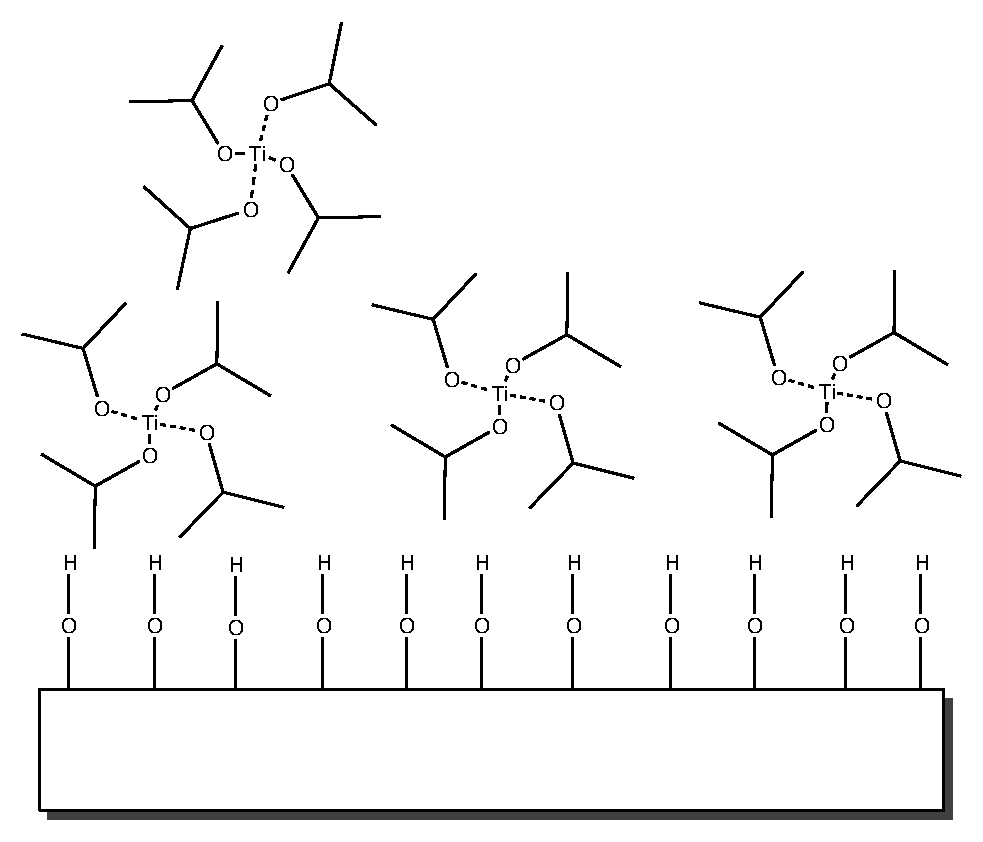
\includegraphics[width=5cm]{./figures/synthesis/chemdraw/a}%
	} 
	\hspace{1cm}
  \subfloat[][Ti Chemisorption]{%
%   	\label{fig:Q50-image}%
	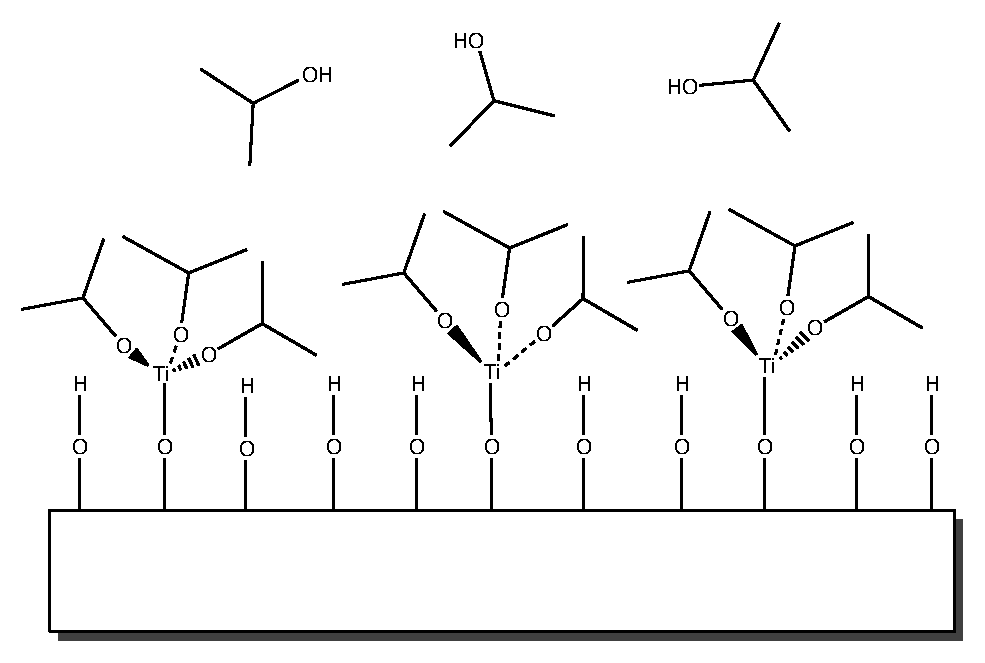
\includegraphics[width=5cm]{./figures/synthesis/chemdraw/b}%
	} \\
  \subfloat[][Ti Ligand Oxidation]{%
%   	\label{fig:Q50-image}%
	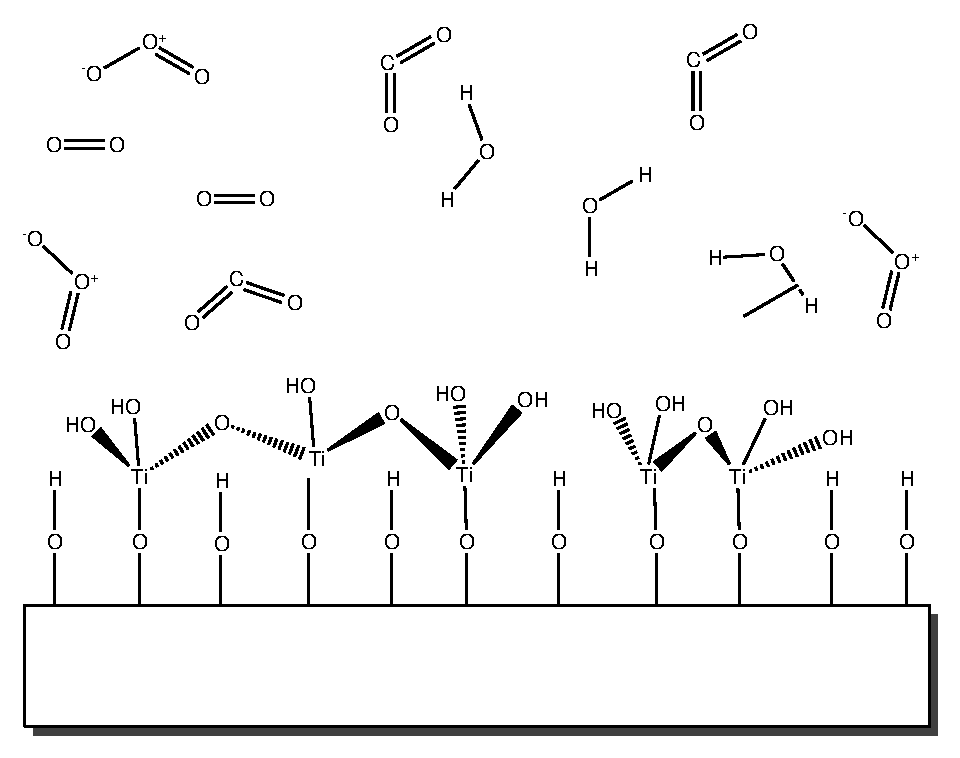
\includegraphics[width=5cm]{./figures/synthesis/chemdraw/c}%
	}  
	\hspace{1cm}	
  \subfloat[][Pb Precursor Injection]{%
%   	\label{fig:Q2000-image}%
	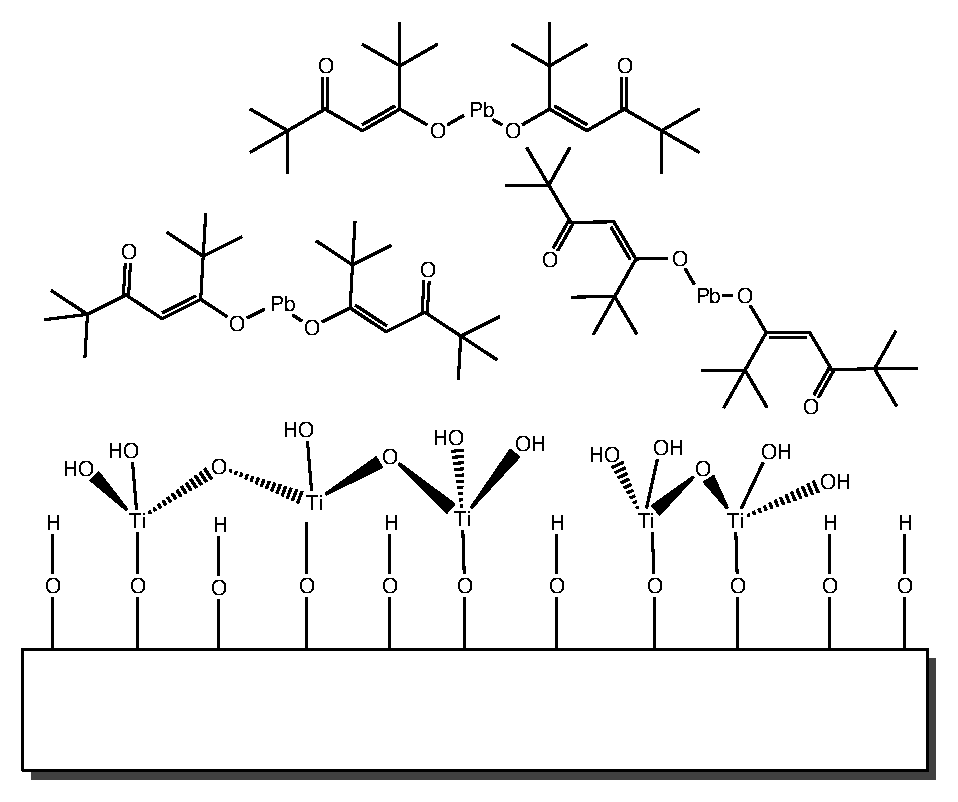
\includegraphics[width=5cm]{./figures/synthesis/chemdraw/d}%
	} \\
  \subfloat[][Pb Chemisorption]{%
%   	\label{fig:Q2000-image}%
	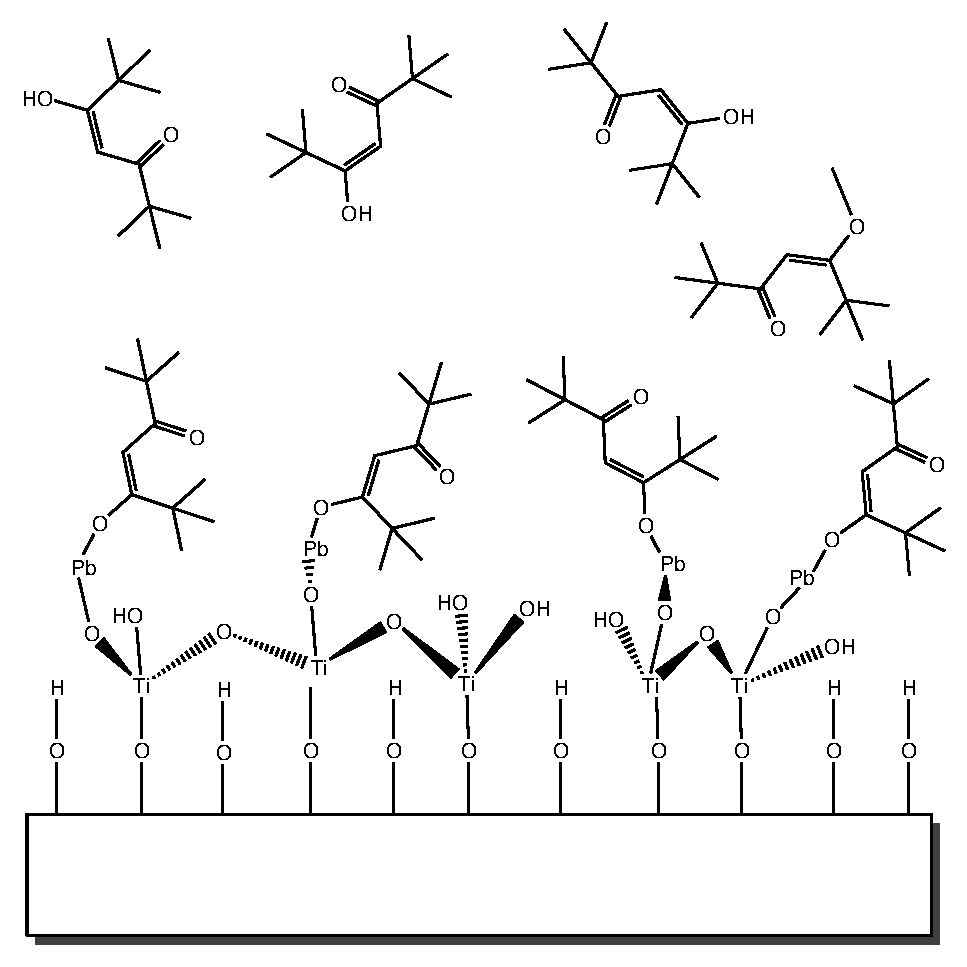
\includegraphics[width=5cm]{./figures/synthesis/chemdraw/e}%
	} 
	\hspace{1cm} 
  \subfloat[][Pb Ligand Oxidation]{%
%   	\label{fig:Q2000-image}%
	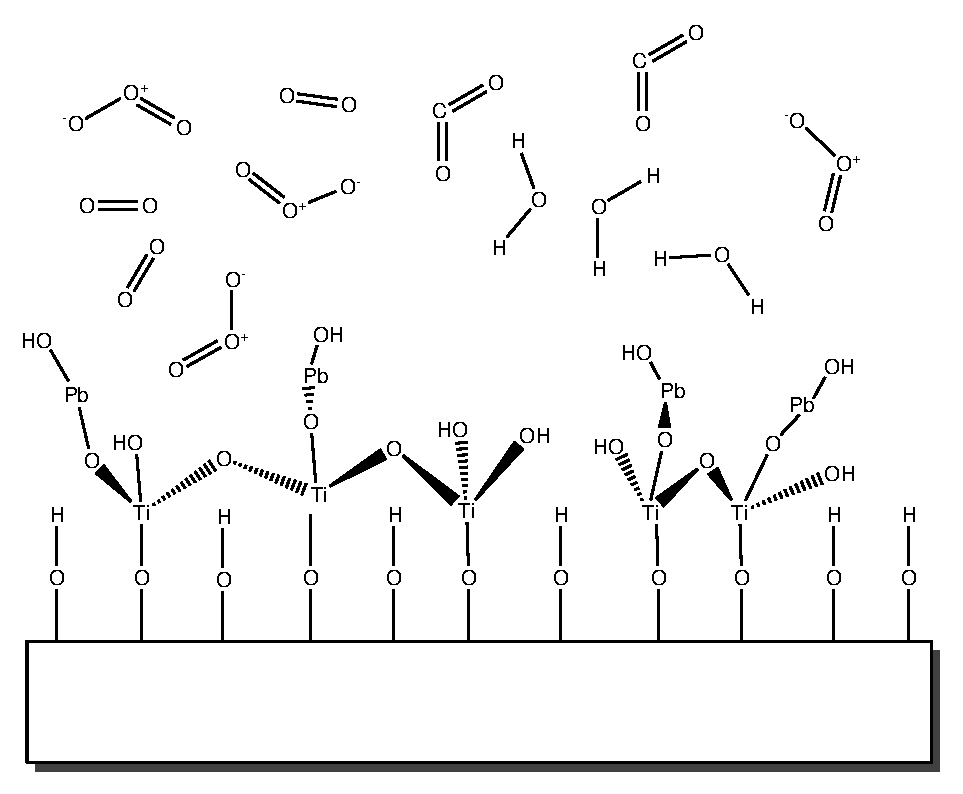
\includegraphics[width=5cm]{./figures/synthesis/chemdraw/f}%
	} \\
  \subfloat[][Completed Cycle, Regenerated Surface]{%
%   	\label{fig:Q2000-image}%
	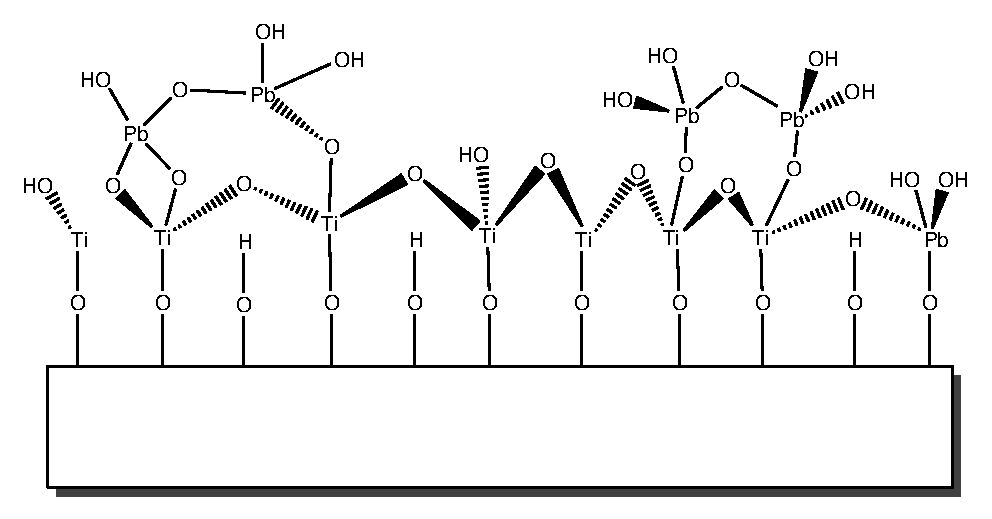
\includegraphics[width=5cm]{./figures/synthesis/chemdraw/g}%
	} 	
   \caption[Illustration of Example \PTO{} ALD Cycle]%
   		{Proposed schematic of \TMHD{} and \TiOiPr{} based ALD deposition for \PTO{}. Purging steps %
		are omitted from this diagram, but would be present between each injection. Steps (d)--(f) would be %
		repeated to incorporate more lead into the film.}
   \label{fig:PTO-pathway}
\end{figure}


%%%%%%%%%%%%%%%%%%%%%%%%%%%%%%%%%%%%%%%%%%%%%%%%%%%%%%%%%%
%%%%%%%%%%%%%%%%%%%%%%%%%%%%%%%%%%%%%%%%%%%%%%%%%%%%%%%%%%
%%%%%%%%%%%%%%%%%%%%%%%%%%%%%%%%%%%%%%%%%%%%%%%%%%%%%%%%%%

\section{Substrate Preparation}
\label{sec:SampFab-Substrates}

Fabrication and preparation of substrates was an important part of the deposition process. Some substrates were purchased and simply cleaned, others needed to be fabricated or otherwise processed prior to cleaning and use in deposition. Three main types of substrates were used: thermally oxidized single-crystalline silicon (100) wafers, silicon wafers that had a thin layer of platinum deposited on the surface, and strontium titanate (100) single crystal substrates. 

%%%%%%%%%%%%%%%
\subsection{Si(100)} \label{sec:Si}

The silicon substrates were prepared in a simple manner. 4 in. diameter silicon wafers with 200 nm of thermally grown oxide (purchased from University Wafer, Inc.\cite{strem_inc}) were diced into 1.5 cm x 1.5 cm pieces. When a sample was to be used for deposition, it was cleaned by one minute of sonication in acetone, followed by isopropanol, with a subsequent 5 minutes of sonication in deionized (DI) water. These were then air dried with dry nitrogen. Finally, the substrates were cleaned in a oxygen plasma cleaning system to remove any remaining organic residues present on the surface.\cite{kern_handbook_1993} 


%%%%%%%%%%%%%%%

\subsection{Platinized Si(100)}

Platinized silicon substrates were prepared in a similar manner to the Si(100) samples. For the initial platinization, a large piece (5 x 5 cm$^{2}$) of pre-cleaned silicon wafer with a thin layer of native oxide, as opposed to the 200 nm of thermally grown oxide, was prepared in the manner described above.\cite{kern_handbook_1993} Then a 15 nm layer of platinum was deposited via ALD.\cite{Ritala_2003_Pt} The substrates were then cleaved into smaller pieces for subsequent use. 

If the samples are stored, it is recommended to again clean the samples in the standard procedure prior to use (see \vref{sec:Si}).

%%%%%%%%%%%%%%%

\subsection{Single Crystal STO(100)}

Single crystal substrates of strontium titanate (\ce{SrTiO3}(100), STO) were purchased from MTI Crystal, Inc.\cite{MTIXtal_inc} as 5 x 5 x 0.5 mm or 10 x 10 x 0.5 mm pieces. These were subsequently processed in such a fashion as to promote the formation of atomically flat terraces. This has the advantage of promoting a uniform surface species across the entire substrate --- the etching process leaves the substrates uniformly titania-terminated.\cite{koster_quasi-ideal_1998}

To achieve the desired surface, the substrates were first pre-cleaned in a four step sonication process. The crystals were cleaned for five minutes in each of acetone, methanol, and isopropyl alcohol. Subsequently, the substrates were sonicated for fifteen minutes in DI water.\cite{koster_quasi-ideal_1998} Next, the substrates were then immersed into a commercially prepared buffered hydrofluoric acid (BHF) solution to etch for 30 seconds, then removed and flushed with copious quantities of DI water to purge any remaining BHF solution.  Once the sample were thoroughly rinsed, they were dried using dry nitrogen. After the etching process, the substrates were annealed at 950\degC{} for one hour.\cite{koster_quasi-ideal_1998} Atomic force microscopy (AFM) was used to confirm the presence of well-defined atomic terraces. 

If the samples are stored, it is recommended to again clean the samples in the standard procedure (see \vref{sec:Si}).

%%%%%%%%%%%%%%%%%%%%%%%%%%%%%%%%%%%%%%%%%%%%%%%%%%%%%%%%%%
%%%%%%%%%%%%%%%%%%%%%%%%%%%%%%%%%%%%%%%%%%%%%%%%%%%%%%%%%%
%%%%%%%%%%%%%%%%%%%%%%%%%%%%%%%%%%%%%%%%%%%%%%%%%%%%%%%%%%

\section{Deposition Parameters}
\label{sec:SampFab-DepParams}

There are four main parameters that can affect the behavior of an ALD deposition.  These are the growth temperature, the dosage of each precursor, the purge time between doses, and any extended precursor-surface exposure time. 

%%%%%%%%%%%%%%%

\subsection{Growth Temperature}

The temperature of the growth chamber has a strong effect on reaction behavior. ALD reactions are sensitive to temperature, and will only proceed properly within a certain range known as the `ALD window.' Outside of this range, the reaction enters one of a number of different regimes; these are determined by comparing the growth rate of the deposition to that of a reaction in the self-limiting saturated ``ALD mode.''\cite{ALD-Handbook,Leskela_2002,lim_atomic_2003,Ritala_ALD_2003} 

If the growth temperature is less than the lower bound of the ALD window, the two regimes are condensation limited and activation energy limited. Condensation limited growth occurs when the substrate temperature is low enough that precursor condenses onto the surface without reacting with the presented sites. This causes higher than expected growth rates, and a lack of self-limiting behavior. If the reaction instead proceeds into the activation energy limited regime, molecules of precursor lack sufficient energy to react with the surface. This is characterized by lower deposition rates.\cite{ALD-Handbook,Leskela_2002} 

Conversely, if the reactor temperature is excessive the reaction again become anomalous. Decomposition limited growth, characterized by excessive deposition, is a result of thermal cracking of the precursor materials. This reaction is not limited to the surface, and accounts for the extra material being deposited. Lower deposition rates indicate that the temperature is sufficient to cause desorption of previously-reacted material from the sample.\cite{ALD-Handbook,Ritala_ALD_2003} 

For an ALD run to be successful, the acceptable temperature window for all of the reactions should overlap in some temperature range. This can become difficult with reactions requiring multiple metal precursors (e.g. \PTO, a combination of \ce{TiO2} and \ce{PbO}), as these can have widely varying ALD windows for their respective reactions. 

%%%%%%%%%%%%%%%

\subsection{Precursor Dosage}

The dosage of precursor or oxidant to the surface is another parameter of critical importance. An ALD reaction requires a minimal amount of precursor to sufficiently saturate the surface, while it is beneficial to minimize any excess precursor as it will be a wasted byproduct (minimizing costs, environmental impact, etc.). 

The vaporization behavior of the precursor can have a dramatic impact on how simple or difficult it is to deliver a saturating dose to the surface. Some materials have readily available precursors with high vapor pressures; titanium isopropoxide and trimethylaluminum (TMA) are both liquids, and tetrakis(dimethylamido)hafnium (\ce{Hf\{N(CH3)2\}4}) is a low-melting temperature solid. These are commonly used precursors for depositing their respective oxides. This vapor pressure becomes an important consideration when choosing a potential compound for use in ALD (as discussed in Section~\vref{sec:SampFab-Precursors}).\cite{ALD-Handbook,kanjolia_design_2008,Leskela_2002,lim_atomic_2003,Ritala_ALD_2003}

Insufficient dosing is apparent in a deposition run by a slower than average growth rate, or also as a non-uniform deposition rate across the sample. However, overdosing is not readily apparent in an ALD-mode deposition. The dose must be lowered to a point where the dose is insufficient, and then increased back to a saturating level. 

Controlling the dose is dependent on injection time (which is the time the valve between the process line and the precursor storage vessel is open), precursor temperature, and the cycle duration (time between precursor injections). By increasing either the injection time or the precursor's temperature the dose is increased, except in some cases with low vapor pressure materials. In this case, it can sometimes be found that the evaporation kinetics are slow and it takes additional time to build up a sufficient amount of vapor to provide a dose to the reactor.\cite{ALD-Handbook,lim_atomic_2003,Ritala_ALD_2003} 

If necessary, multiple doses of precursor can be delivered to the sample during each cycle to increase the total delivered dose.

%%%%%%%%%%%%%%%

\subsection{Purge Time}

Purge time is important as it gives time for the \ce{N2} flow to flush any remaining byproducts, excess reactants, and physisorbed (as opposed to chemisorbed) species from the substrate surface and out of the reactor zone. It also allows time between cycles which allows for low vapor pressure precursors to regenerate evaporated material; if this time is too short to fully regenerate the dose in the cylinder the precursor will eventually appear to be depleted during the course of the deposition.\cite{ALD-Handbook,Leskela_2002}

%%%%%%%%%%%%%%%

\subsection{Exposure Time}

Exposure time denotes the time where the precursor is held in the reaction zone to increase the amount of time during which the surface reaction can occur. This is beneficial for two types of depositions. In the case of low-reactivity precursors, it increases the amount of time that the precursor is available to the surface, greatly increasing the surface coverage per cycle. Exposure mode is also beneficial for depositing upon three dimensional structures, especially those with a high aspect ratio, e.g. nanotube templates. This extra dwell time of the precursor allows for diffusion of reactant into the structure, for a uniform coverage upon the entirety of the surface. Purge time must be increased accordingly to allow for byproducts to diffuse back out of the structure.\cite{ALD-Handbook,gordon_kinetic_2003,Leskela_2002}

%%%%%%%%%%%%%%%%%%%%%%%%%%%%%%%%%%%%%%%%%%%%%%%%%%%%%%%%%%
%%%%%%%%%%%%%%%%%%%%%%%%%%%%%%%%%%%%%%%%%%%%%%%%%%%%%%%%%%
%%%%%%%%%%%%%%%%%%%%%%%%%%%%%%%%%%%%%%%%%%%%%%%%%%%%%%%%%%

\section{Post-Deposition Annealing}
\label{sec:SampFab-Annealing}

Two types of annealing procedures were used in this study. Oven annealing, with the simple use of a furnace in ambient atmosphere; and rapid thermal annealing (RTA), characterized by very high heating and cooling rates and performed in an inert atmosphere (dry \ce{N2}). 


%%%%%%%%%%%%%%%

\subsection{Oven Annealing}

In oven annealing, the samples to be processed are placed in a cold oven in the ambient atmosphere of the laboratory. The samples are then heated gradually at a rate of 10--25\degC{} per minute up to the final annealing temperature, which ranged from 600--900\degC{}. The samples are then allowed to heat-treat for 120 minutes at the process temperature, and then the furnace is allowed to return to room temperature. 

This conventional heating pattern allows the sample to obtain its equilibrium crystalline phase composition, be that a single crystalline phase, polycrystalline, or involve multiple phases or materials. This was the annealing method most commonly used during this study. 

%%%%%%%%%%%%%%%

\subsection{Rapid Thermal Annealing}

Rapid thermal annealing (RTA), as its name suggests, involves very high heating and cooling rates. RTA systems can heat at rates over 10\degC{} per second, allowing the chamber and sample to reach the process temperature very quickly. Similarly, processing times are generally much shorter, and are generally no longer than 10--15 minutes. Cooling, facilitated by a water cooling apparatus, also occurs rapidly. These sharp gradients can have different effects on the crystal structure of the film, locking in different phases in the material that may otherwise dissociate given more time during heating or cooling. 

In this study samples processed via RTA used a HeatPulse\textsuperscript{\texttrademark} RTA system, which allowed for automatic control of the process. Sample processing conditions can be found in table~\vref{tbl:LoSamples}. 






\chapter{Material Characterization}
\label{chap:Charact}
\thispagestyle{empty}

%%%%%%%%%%%%%%%%%%%%%%%%%%%%%%%%%%%%%%%%%%%%%%%%%%%
%%%%%%%%%%%%%%%%%%%%%%%%%%%%%%%%%%%%%%%%%%%%%%%%%%%
%%%%%%%%%%%%%%%%%%%%%%%%%%%%%%%%%%%%%%%%%%%%%%%%%%%

\section{Thermal Analysis}
\label{sec:Charact-Thermal}

%%%%%%%

\subsection{Thermogravimetric Analysis}

Thermogravimetric analysis (TGA) is a very useful tool when attempting to determine the viability of a precursor in an ALD process. It allows for estimation of vaporization rate at various temperature rates as well as indications of chemical breakdown (i.e. thermalization) which would hinder the precursor's usefulness. 

At its core, TGA is a measurement of mass loss as a function of temperature or time. A small sample (1--10 mg) of material is placed in a microgram balance pan and suspended inside a furnace. The furnace is then heated at a specified rate while the sample mass is carefully monitored. For the experiments used in this study (evaluation of thermal vaporization and thermal degradation) it is important to ensure that the testing environment is inert. This is accomplished by using a platinum pan in the microgram balance and constantly purging the furnace with a small flow of dry nitrogen gas. The heating rate can be varied according to a pre-determined program to provide more information at various individual temperatures.\cite{Broido_TGA_1969,Doyle_TGA_1961,horowitz_TGA_1963,wunderlich_thermal_1990} 

This technique was used to evaluate various precursor candidates for the lead oxide half of the \PTO{} deposition procedure. The instrument used was a Q50 TGA device (fig.~\vref{fig:Q50-image}).  A detailed discussion of TGA procedures and the investigated chemicals can be found in subsequent chapters (see \vref{sec:SampFab-Precursors} and \vref{chap:Results-Thermal}). 

\begin{figure}[tb]
   \centering
   \subfloat[Q50 TGA][Q50 TGA]{%
   	\label{fig:Q50-image}%
	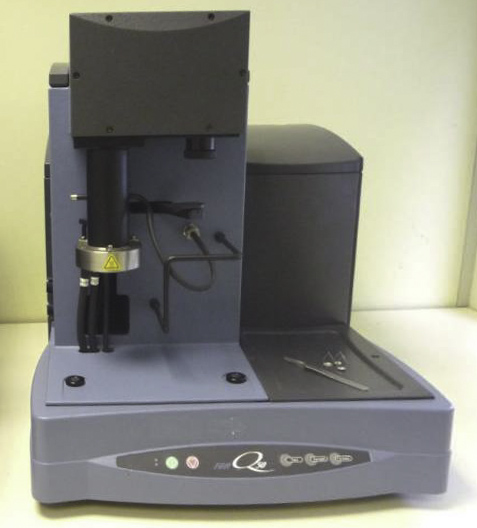
\includegraphics[width=0.45\linewidth]{./figures/characterization/Q50-TGA}%
	} 
  \subfloat[Q2000 DSC][Q2000 DSC]{%
   	\label{fig:Q2000-image}%
	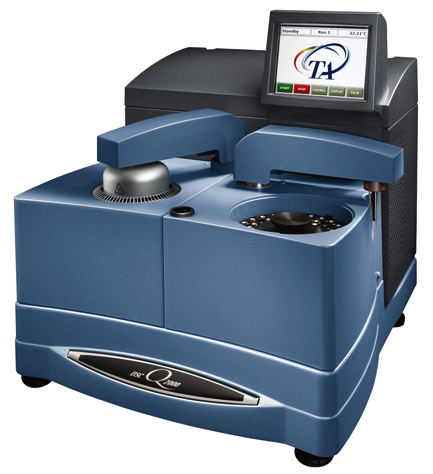
\includegraphics[width=0.45\linewidth]{./figures/characterization/Q2000-DSC}%
	} 	
   \caption[T.A. Instruments, Inc. Instrumentation]%
   		{Photograph of the thermal analysis instrumentation used during this study, \\
		made by T.A.  Instruments, Inc.\\%
		{\tiny Image Sources: (a) \url{http://mrc.stu.edu.cn/old/Chinese/Resource/Equipments/TGA.htm} %
		via Go-Dove.com.\cite{go-dove}%
		\\%
		(b) \url{http://www.go-dove.com/en/event-16047/lot-213/TA-Instruments-Q50-Thermo-Gravimetric-Analyser} \\%
		from Semiconductor-Technology.com.\cite{Semiconductor-tec}}}
   \label{fig:TA-Instruments}
\end{figure}

%%%%%%%

\subsection{Differential Scanning Calorimetry}
	
Differential scanning calorimetry (DSC) is a technique that allows for the determination of various critical temperatures for a material, and also can highlight changes in chemical structure due to degradation or other thermal processes. 

DSC is the analysis of energy absorption as a function of temperature, which is the essence of calorimetry. DSC uses a sample and reference system to isolate the energy absorbed by the sample from that of the holder pan. Sample sizes usually range from 0.1--2 mg of material; as the samples used in this study are volatile the sample pans are hermetically sealed to prevent mass loss. The sample and reference pans are then placed inside a thermally insulated chamber. The temperature of each is carefully monitored, and differing amounts of heat are applied to negate the temperature difference between the sample and reference. The difference in absorbed heat as a function of temperature is then given as the result. In general, experiments include both heating and cooling curves to gain a complete understanding of the different energies.\cite{oneill_DSC_1964,skoog_DSC_1998,wunderlich_thermal_1990} 
	
DSC was used to analyze the behavior of precursor chemicals around their evaporation and reaction temperatures. The main goal was to determine if the material underwent any thermally-activated degradation processes at either of these two temperature ranges. At the evaporation temperature, the sample was generally cycled multiple times to simulate actual use in the ALD. These measurements were taken using a Q2000 DSC system (fig.~\vref{fig:Q2000-image}) made by T.A. Instruments, Inc.	

%%%%%%%%%%%%%%%%%%%%%%%%%%%%%%%%%%%%%%%%%%%%%%%%%%%
%%%%%%%%%%%%%%%%%%%%%%%%%%%%%%%%%%%%%%%%%%%%%%%%%%%
%%%%%%%%%%%%%%%%%%%%%%%%%%%%%%%%%%%%%%%%%%%%%%%%%%%

\section{Thin Film Characterization}
\label{sec:Charact-ThinFilm}


%%%%%%%
	
\subsection{Variable Angle Spectroscopic Ellipsometry}

Ellipsometry is a powerful non-destructive optical technique that allows for the determination of a large number of properties of complex thin film structures. The basic tenet of ellipsometry relies on the analysis of the change in polarization state of a reflected light beam after interaction with the sample. The incident beam is generally linearly polarized, but upon reflection becomes elliptically polarized due to a phase shift in the components of the beam in the s- and p-plane, as well as a change in their relative amplitudes. The phase shift is correlated to the ellipsometric parameter $\Delta$, while the amplitude change is given by $\tan\Psi$ ($\Psi$ is the angle between the s-plane and the major axis of the ellipse). The last major parameter is the incident angle, denoted by $\Phi$. A schematic diagram illustrating these parameters can be seen in figure~\vref{fig:ellipsometry}.\cite{azzam_ellipsometry_1987,schubert_infrared_2005,tompkins_spectroscopic_1999} 

\begin{figure}[tb]
   \centering
   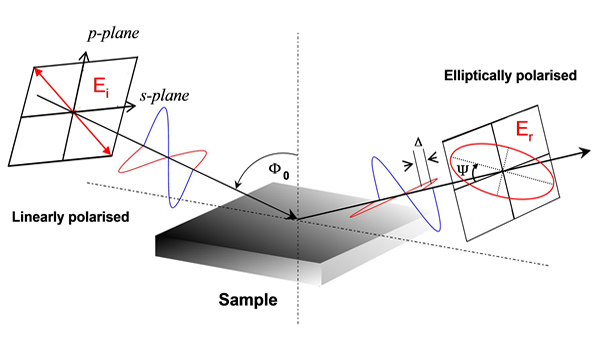
\includegraphics[width=\linewidth]{./figures/characterization/ellipsometryDiagram_simple} 
   \caption[Ellipsometric Beam Path and Modeling Parameters]{Schematic of the beam path during an %
   					ellipsometric measurement, \\ critical parameters are indicated.\\
					{\tiny Image source: \url{http://www.tcd.ie/Physics/Surfaces/ellipsometry2.php} %
					from Trinity College of Dublin.\cite{trinity_college_dublin}}}
   \label{fig:ellipsometry}
\end{figure}

From these parameters, one can directly determine the ratio between the reflectance in the p-plane ($r_{p}$) and the reflectance in the s-plane ($r_{s}$) from the fundamental ellipsometric relation (eqn.~\vref{eq:ellipsometry}).  Once this relationship is known, the Fresnel equations (eqn.~\vref{eq:fresnel}) can be used to numerically determine the value of the complex index of refraction at the specific wavelength of the incoming beam. The complex index of refraction (eqn.~\vref{eq:complexindex}) describes the nominal index of refraction but additionally includes an imaginary term to describe absorption of light in the material (commonly referred to as the extinction coefficient, $\kappa$).\cite{azzam_ellipsometry_1987,schubert_infrared_2005,tompkins_spectroscopic_1999}  

\begin{equation}
 \label{eq:ellipsometry}
 \displaystyle
	\rho(\lambda) = \frac{\tilde{r}_{p}(\lambda)}{\tilde{r}_{s}(\lambda)} = \tan(\Psi(\lambda))e^{i\Delta(\lambda)}
\end{equation}

\begin{subequations}
\label{eq:fresnel}
\begin{align}
	r_{p}(\lambda) &= \frac{\tilde{n}_{1}(\lambda)\sqrt{1- \left(\frac{\tilde{n}_{1}(\lambda)}{\tilde{n}_{2}(\lambda)}\sin\Phi\right)} - \tilde{n}_{2}(\lambda)%
			\cos\Phi}{\tilde{n}_{1}(\lambda)\sqrt{1- \left(\frac{\tilde{n}_{1}(\lambda)}{\tilde{n}_{2}(\lambda)}\sin\Phi\right)} + %
			\tilde{n}_{2}(\lambda)\cos\Phi} \\
        	r_{s}(\lambda) &= \frac{\tilde{n}_{1}(\lambda)\cos\Phi - \tilde{n}_{2}(\lambda)\sqrt{1- \left(\frac{\tilde{n}_{1}(\lambda)}{\tilde{n}_{2}(\lambda)}\sin\Phi\right)}}%
			{\tilde{n}_{1}(\lambda)\cos\Phi + \tilde{n}_{2}(\lambda)\sqrt{1- \left(\frac{\tilde{n}_{1}(\lambda)}{\tilde{n}_{2}(\lambda)}\sin\Phi\right)}}
\end{align}
\end{subequations}

\begin{equation}
 \label{eq:complexindex}
 \displaystyle
	\tilde{n}(\lambda) = n(\lambda)+ i\kappa(\lambda)
\end{equation}

This type of analysis is sufficient for thick, isotropic samples without any surface layers (e.g. surface oxides or adsorbed gases), and can directly provide the value of $\tilde{n}$ as a function of $\lambda$. However, once layers are stacked upon one another, the system becomes very difficult to analyze directly due to interference effects between the layers, especially at varying wavelengths. It becomes necessary to use modeling techniques to determine the correct values of $\tilde{n}(\lambda)$ and thickness ($t$) for each layer.\cite{schubert_infrared_2005,tompkins_spectroscopic_1999} 

The power of ellipsometry as a high-resolution optical analysis technique stems from the use of phase and polarization changes. This allows the analysis to overcome the diffraction limit, and can be accurate down to angstroms. Properly modeling the system is critical for this analysis to be as precise as possible. Thus, there have been refinements of the ellipsometric method to greatly increase the amount of experimental data points, allowing the overall system to be over-determined and thus letting all of the systems parameters to be calculated. 
	
Variable angle spectroscopic ellipsometry (VASE) is one of these variants. Spectroscopic ellipsometry differs from single-wavelength ellipsometry by utilizing a broad-band light source as opposed to a monochromatic source. By performing ellipsometric analysis at each of the wavelengths, one can determine the wavelength (and thus photon-energy) dependence of $n$ and $\kappa$. This not only helps to improve data analysis (as it can generally be safely assumed that the values of $n$ and $\kappa$ are smooth functions of $\lambda$), but allows for the determination of many other properties of the material. Of specific importance is the complex dielectric function ($\tilde{\epsilon}$), which is related to $\tilde{n}$ by the relation shown in equation~\vref{eq:dielectricfunction}. Knowing these functions can allow for determination of electronic properties such as the bandgap energy, the absorption coefficient, amongst others. Finally, by obtaining spectra at a number of different incident angles, one directly provides additional data points across the entire wavelength spectrum. Even a small number of additional angles can quickly provide sufficient data points for the system to be over determined.\cite{azzam_ellipsometry_1987,schubert_infrared_2005,tompkins_spectroscopic_1999} 

\begin{equation}
 \label{eq:dielectricfunction}
 \displaystyle
	\tilde{\epsilon} = \epsilon_{1} + i\epsilon_{2} = \tilde{n}^{2}
\end{equation}

During this project, a VASE M-2000U system (figure~\vref{fig:M2000_image}) built by J.A. Woollam, Inc. was used to collect all of the ellipsometric data. In addition, data analysis was performed using the WVASE32{$^{\copyright}$} package also provided by J.A. Woollam, Inc. The system utilizes a rotating compensator and a CCD detector to greatly decrease data collection time by collecting data across the entire spectrum simultaneously.  More information on this system is available from the J.A. Woollam, Inc. webpage.\cite{woollam-web}

\begin{figure}[tbp]
   \centering
   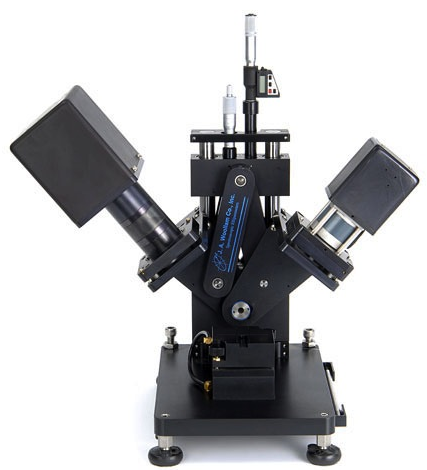
\includegraphics[width=0.5\linewidth]{./figures/characterization/M2000_ellipsometer_image.png} 
   \caption[J.A. Woollam M-2000U Ellipsometer]%
   		{Photograph of the J.A. Woollam M-2000U variable \\%
   		 angle spectroscopic ellipsometer (VASE).\\%
		 {\tiny Image Source: \url{http://jawoollam.com/Gallery/m2000_manual2.html} from J.A. Woollam, Inc.%
		 \cite{woollam-web}}}
   \label{fig:M2000_image}
\end{figure}


%%%%%%%%%%%%%%%%%%%%%%%%%%%%%%%%%%%%%%%%%%%%%%%%%%%
%%%%%%%%%%%%%%%%%%%%%%%%%%%%%%%%%%%%%%%%%%%%%%%%%%%
%%%%%%%%%%%%%%%%%%%%%%%%%%%%%%%%%%%%%%%%%%%%%%%%%%%



\section{Compositional Analysis}
\label{sec:Charact-Comp}

%%%%%%%
\subsection{Energy-Dispersive X-Ray Spectroscopy}

Energy dispersive X-ray spectroscopy (EDXS) is a commonly used analysis technique for determining the composition of a sample. In this process, a sample is bombarded with high-energy electrons (2--30 keV) which interact with the sample. Some of these electrons will cause a core electron of an atom in the sample to be ejected. This leaves a vacant orbital in the inner shell, which a higher energy electron will fill. In the process of filling the vacancy, the electron will emit an X-ray photon equal to the energy difference between the two states. These energies are referred to using the common X-ray spectroscopy nomenclature (e.g. $K_{\alpha}$, $K_{\beta}$, $L_{\alpha}$). An illustration of this process can be found in figure~\vref{fig:EDXS-image}.\cite{goldstein_EDS_2003}  

Since the energies of the emitted photons are very specific to each element, the procedure can be used to identify the presence of the element in the sample. With some calibration, EDXS can also be used to quantify the relative amounts of each element in a sample using the different number of collected photons. However, this can sometimes be difficult due to some elements have overlapping spectrums as the peaks are not sharp and different elements can have similar energies for some transitions.\cite{goldstein_EDS_2003} 

One of the downsides of EDXS is that the interaction volume of electrons is much larger deeper into the sample, so the surface sensitivity of the technique is smaller than with some other techniques. Additionally, Bremsstrahlung radiation, which is caused by high-energy electrons interacting with other charged particles, provides a large degree of background noise which can drastically interfere with the techniques ability to precisely measure, or even identify, trace elements such as those in a thin film.\cite{goldstein_EDS_2003}

\begin{figure}[tb]
   \centering
   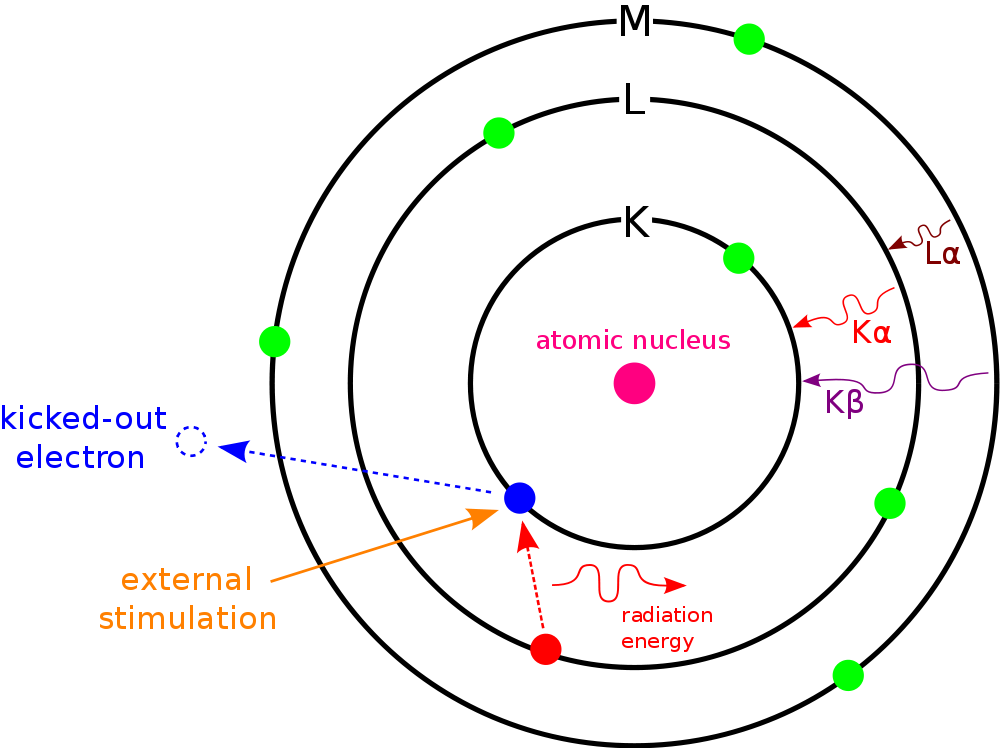
\includegraphics[width=0.66\linewidth]{./figures/characterization/EDXS-scheme} 
   \caption[Illustration of EDXS principle]%
   		{Graphic illustrating the basic mechanism for EDXS, along with the commonly used %
		notation for the various energies. The external stimulation would be a high energy %
		electron. \\{\tiny Image source: \url{http://commons.wikimedia.org/wiki/File:EDX-scheme.svg} originally %
		contributed by ``Muso'' under GFDL license.}}
   \label{fig:EDXS-image}
\end{figure}



%%%%%%%

\subsection{X-Ray Fluorescence Spectroscopy}

X-ray fluorescence spectroscopy (XRFS) is a similar technique to EDXS. In XRFS the excitation used is X-ray photons (often from a Cu K$_{\alpha}$ source with $\lambda = 1.54$ \AA), as opposed to energetic electrons. In other considerations the techniques are equivalent. 

XRFS has a lower noise floor than EDXS, due to the lack of signal from Bremsstrahlung radiation from the deceleration of electrons, allowing smaller signals to be more easily identified (such as in ultra-thin films). It does suffer the same disadvantage of having overlapping peaks. This resolution issue can be alleviated to some degree by using wavelength dispersive XRFS (WD-XRFS), which uses diffraction techniques to analyze the emitted x-ray spectrum.\cite{Vincze_XRF_2005} 

X-ray fluorescence spectroscopy was performed using a fX-SEM analysis system from iXRF Systems, Inc.\cite{iXRF-web}  It was the primary method of composition analysis for the results presented in this thesis.



%%%%%%%%%%%%%%%%%%%%%%%%%%%%%%%%%%%%%%%%%%%%%%%%%%%
%%%%%%%%%%%%%%%%%%%%%%%%%%%%%%%%%%%%%%%%%%%%%%%%%%%
%%%%%%%%%%%%%%%%%%%%%%%%%%%%%%%%%%%%%%%%%%%%%%%%%%%
	
\section{Phase Identification}
\label{sec:Charact-PhaseID}

%%%%%%%

\subsection{X-Ray Diffraction}

X-ray diffraction (XRD) is a very commonly used technique for performing this identification. Utilizing the concepts of coherent interference, which leads to Bragg's law of diffraction given in equation~\vref{eq:braggs-law}. X-rays are utilized because their wavelengths are similar to the length scales between atomic planes in crystals (1--100\AA). As the incident rays pass through the sample and are reflected by atomic planes, they can either constructively or destructively interfere.\cite{giacovazzo_XRD_1992} 

\begin{equation}
 \label{eq:braggs-law}
 \displaystyle
	n\lambda = 2d\sin\theta
\end{equation}

Figure~\vref{fig:braggs-law} gives a graphical illustration of this principle. If the extra distance traversed by photons on the first path is equal to an integer number of wavelengths there will be constructive interference (see fig.~\vref{fig:bragg-constructive}). However, if the $\theta$ angle is slightly changed the interference rapidly obtains destructive character (see fig.~\vref{fig:bragg-destructive}). In this manner, if the crystal is moved through a range of $\theta-2\theta$ values, a pattern of angles where constructive interference occurred. \cite{giacovazzo_XRD_1992}

\begin{figure}[tbp]
   \centering
   \subfloat[Constructive Interference][Constructive Interference]{%
   	\label{fig:bragg-constructive}%
	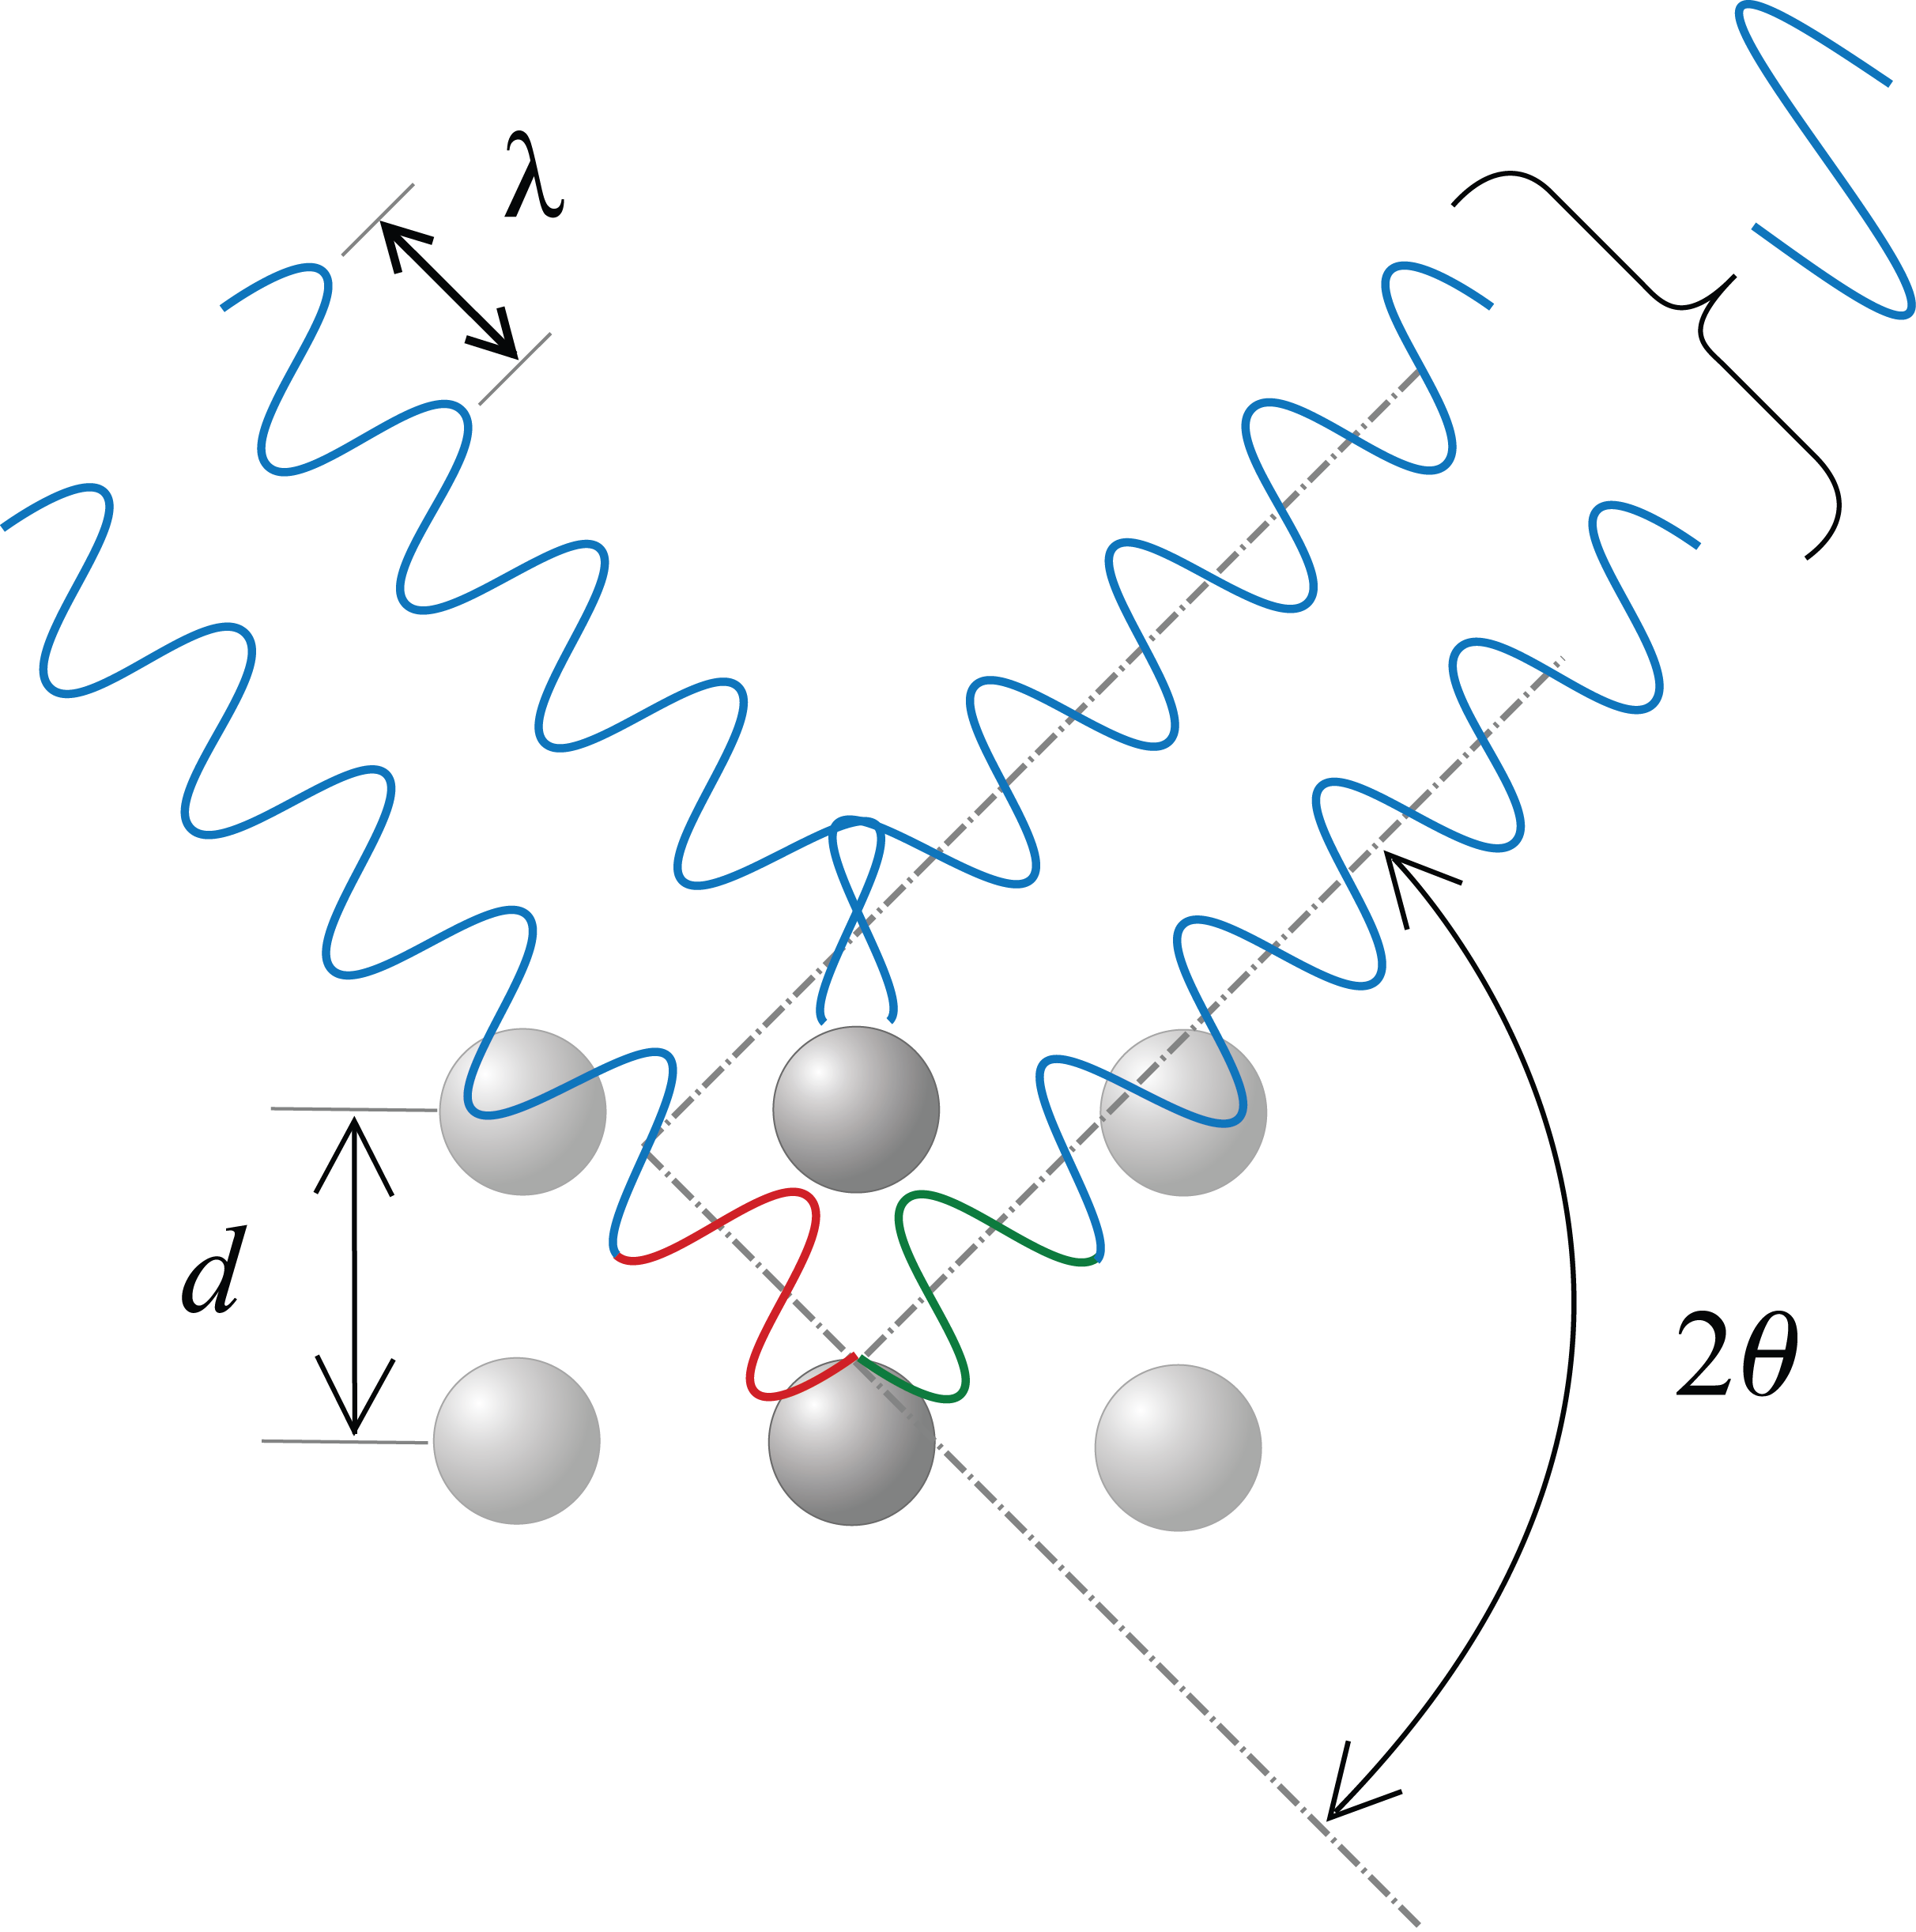
\includegraphics[width=0.475\linewidth]{./figures/characterization/bragg-diffraction-constructive}%
	} 
	\hspace{0.5cm}
  \subfloat[Destructive Interference][Destructive Interference]{%
   	\label{fig:bragg-destructive}%
	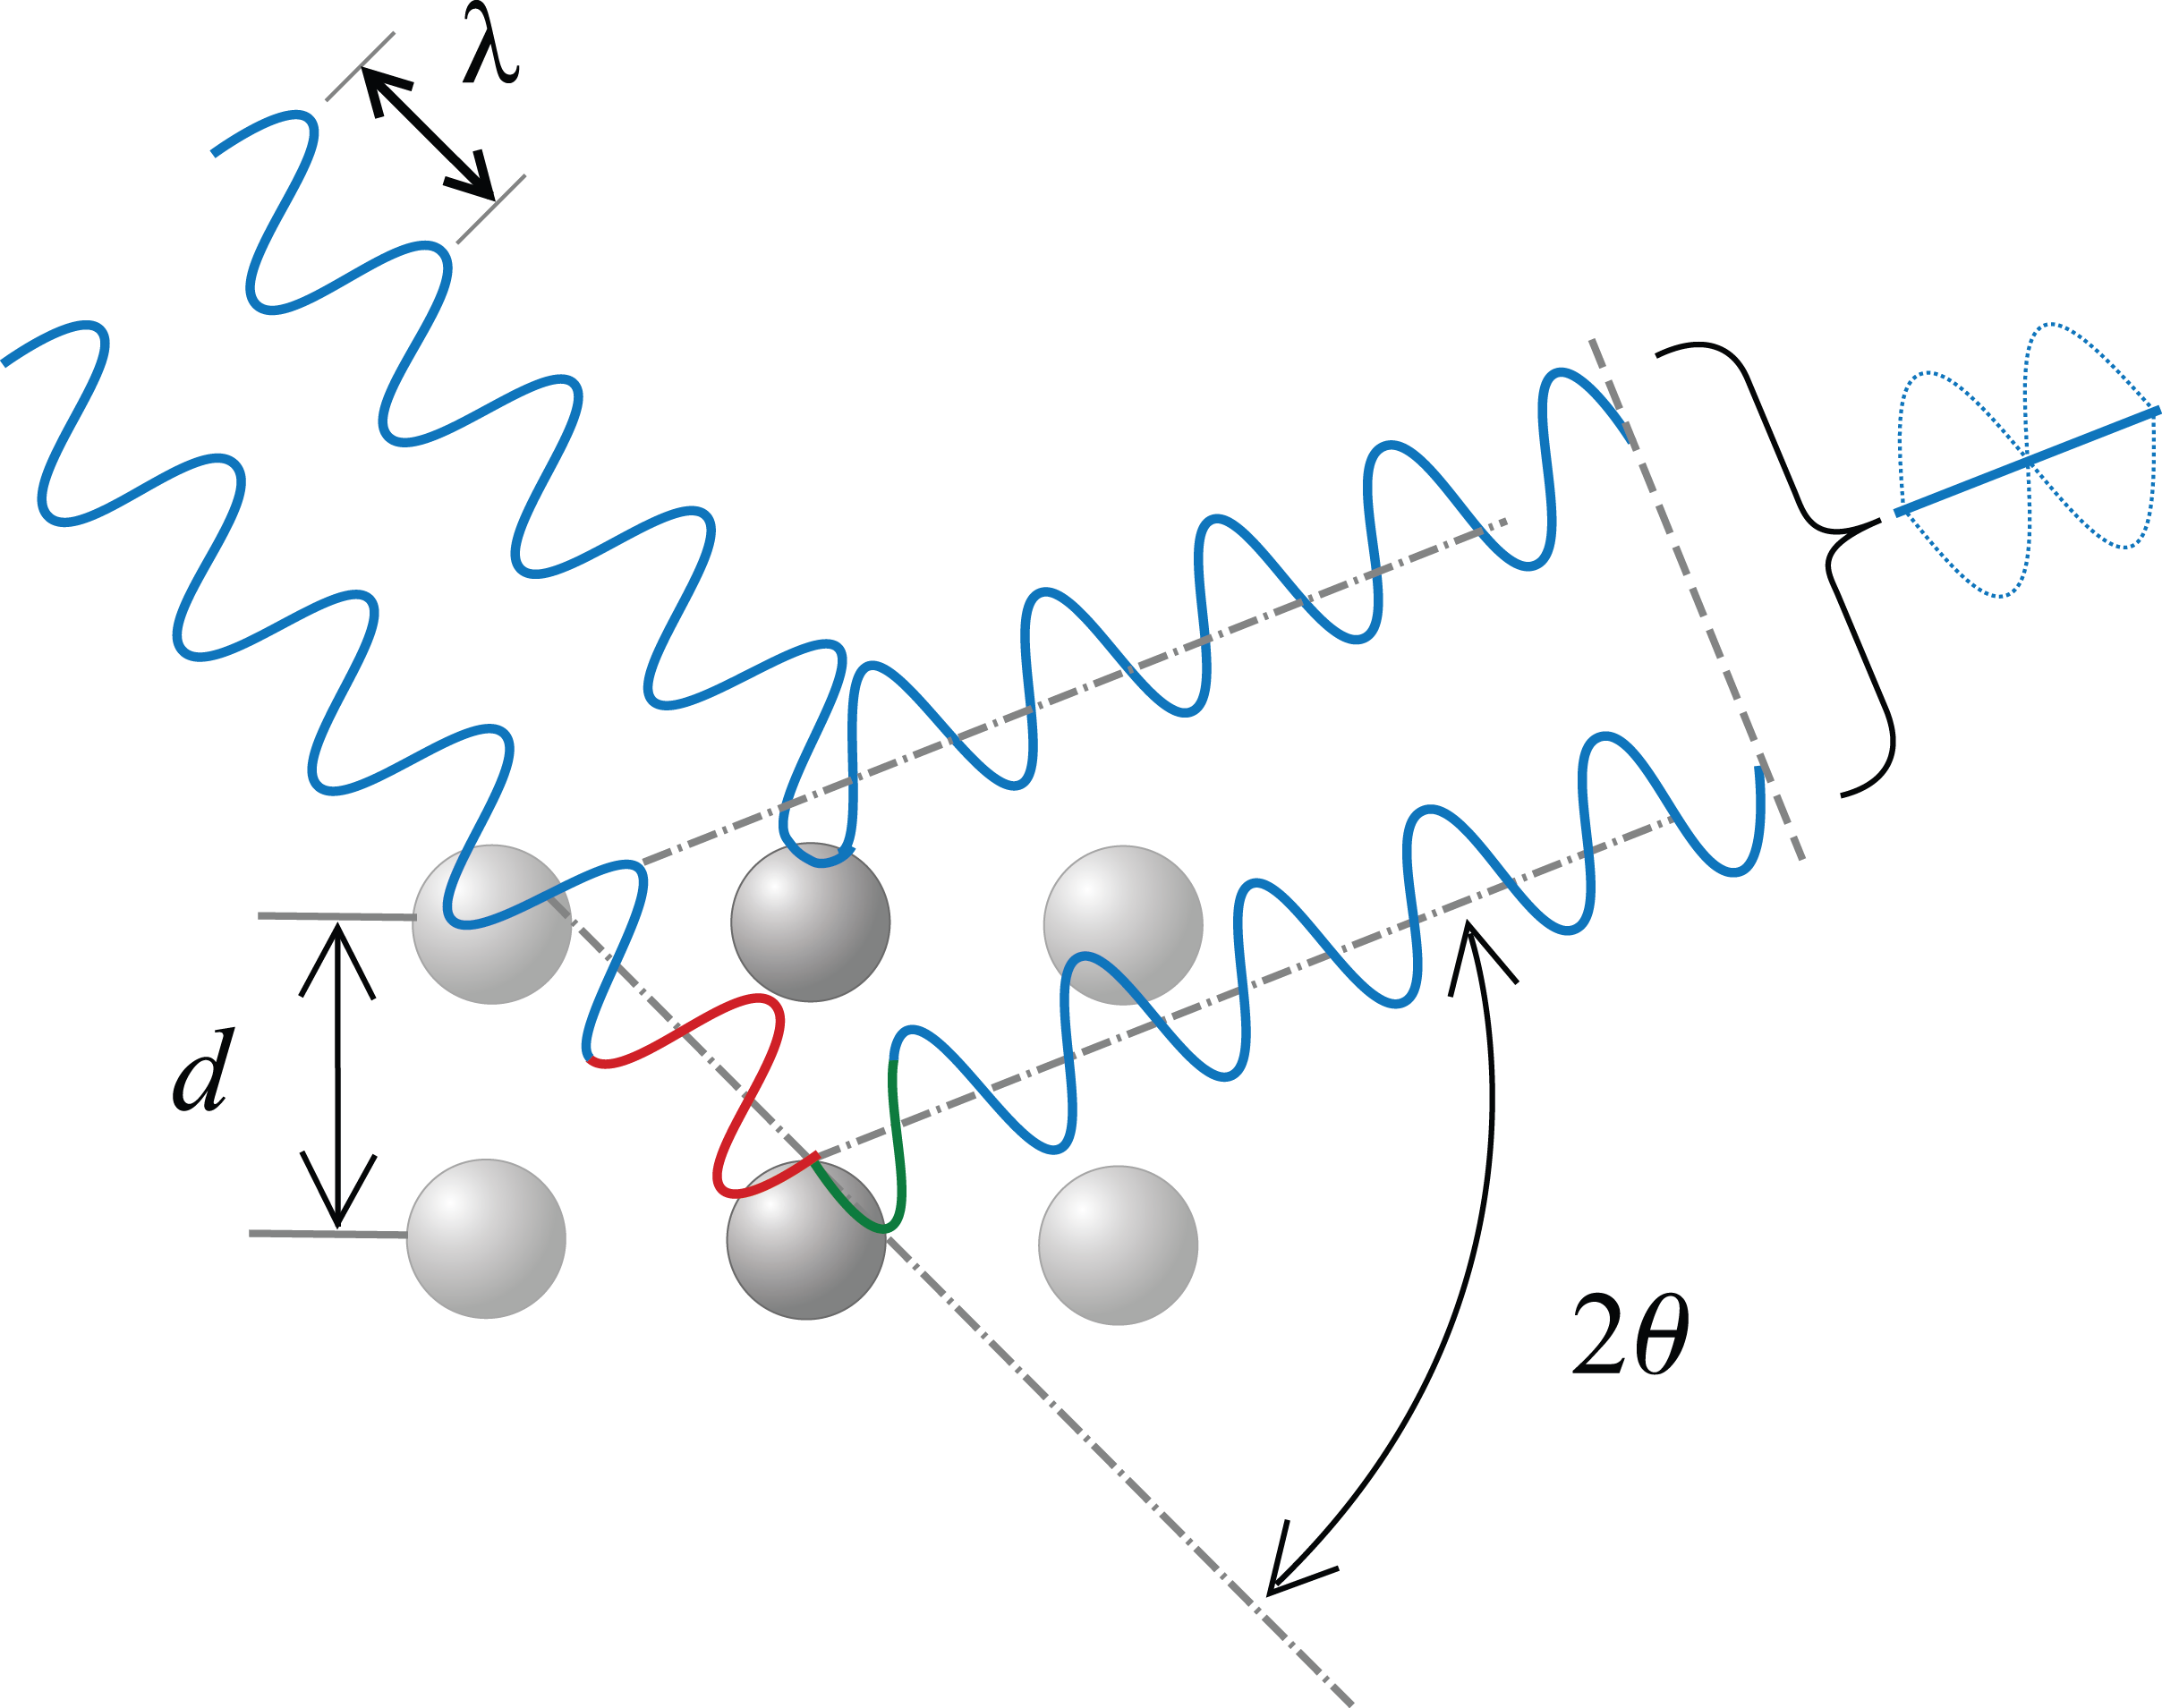
\includegraphics[width=0.475\linewidth]{./figures/characterization/bragg-diffraction-destructive}%
	} 	
   \caption[Illustration of Bragg's Law]%
   		{These two images illustrate the effect of interference on Bragg diffraction. In (a) the extra %
		path length is exactly correct to allow coherence with the other ray; this causes constructive %
		interference. (b) is the other condition, where the path length causes a phase shift of 90\Deg{}%
		and thus the rays interfere destructively.\\%
		{\tiny Image Source: \url{http://en.wikipedia.org/wiki/File:Braggs_Law.svg} originally contributed by %
		``Cdang'' under CCA-Share Alike 3.0 License}}
   \label{fig:braggs-law}
\end{figure}

The diffraction pattern can be used to determine a list of the interplane spacings (d-spacings) present in the sample. The values of peaks at various 2$\theta$ can be converted to d-spacings via the relation $d=\frac{\lambda}{2\sin\theta}$. Individual materials will have a specific pattern of reflections that allow them to be identified in the sample.\cite{giacovazzo_XRD_1992} 

This project used a Rigaku SmartLab XRD (see figure~\vref{fig:rigaku-smartlab-photo}), which utilized a Cu-K$_{\alpha}$ X-ray source ($\lambda = 1.5418$\AA).

%\begin{figure}[tbp]
%   \centering
%   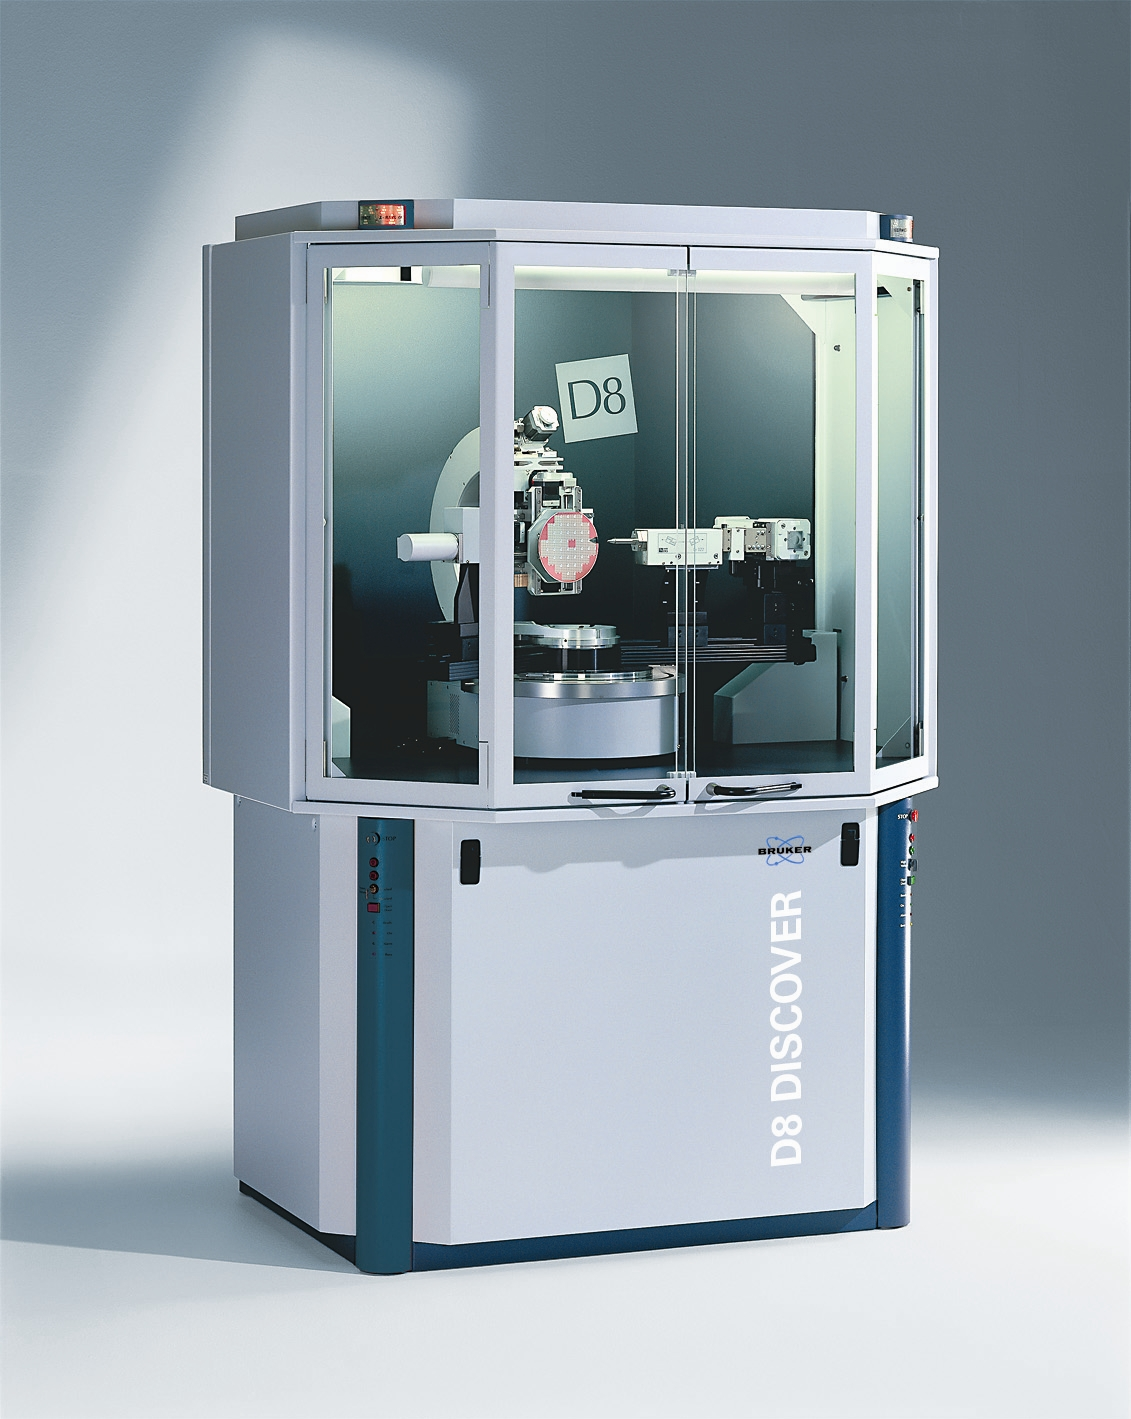
\includegraphics[width=0.5\linewidth]{./figures/characterization/bruker-d8-photo.jpg} 
%   \caption[Bruker D8 Discover XRD]%
%   		{Photograph of the Bruker D8 Discover X-ray diffractometer}
%   \label{fig:bruker-d8-photo}
%\end{figure}

\begin{figure}[tbp]
   \centering
   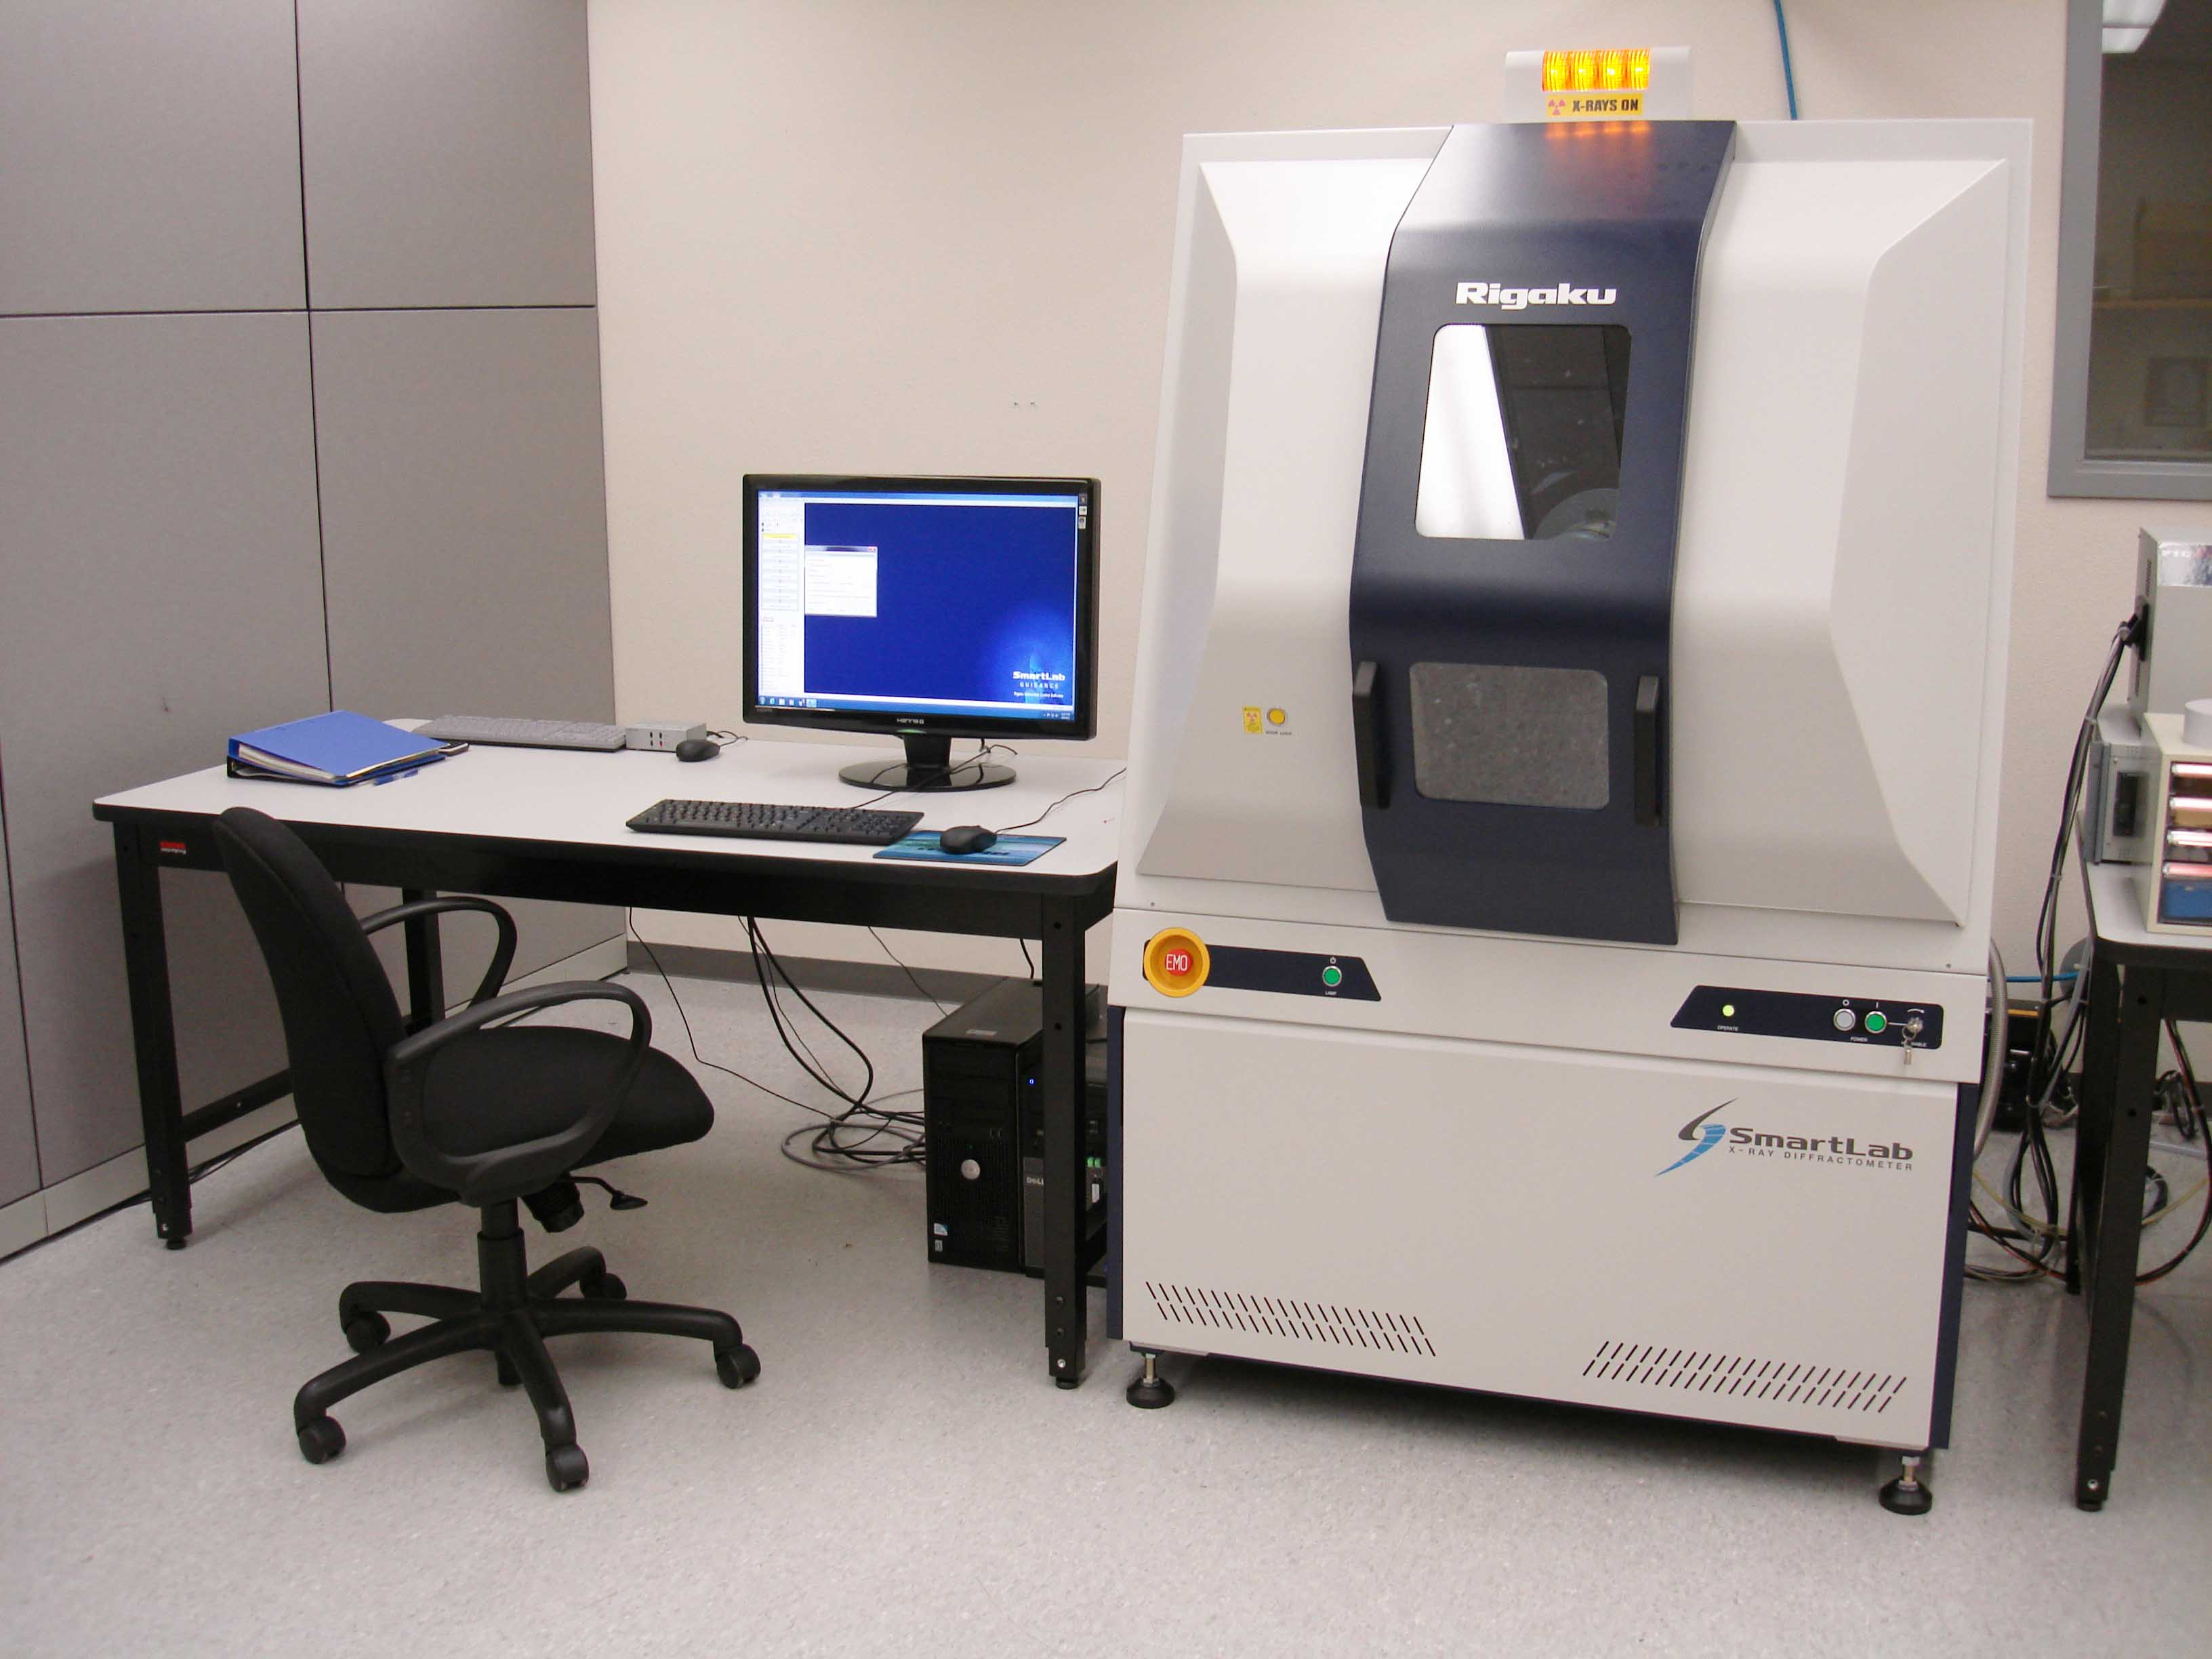
\includegraphics[width=0.75\linewidth]{./figures/characterization/rigaku-smartlab-photo.jpg} 
   \caption[Rigaku SmartLab XRD]%
   		{Photograph of the Rigaku SmartLab X-ray diffractometer.\\%
		{\tiny Image Source: \url{http://lexi.eng.uci.edu/facilities.html} from the University of California - Irvine%
		\cite{smartlab-image}}}
   \label{fig:rigaku-smartlab-photo}
\end{figure}


%%%%%%%

%\subsection{Grazing Incidence X-Ray Diffraction}
%
%Both instruments used in this study were capable of collecting data in GIXRD mode (fixed $\omega$--2$\theta$). 


































	
	
	
\chapter{Analysis Methods}
\label{ch:Methods}
\thispagestyle{empty}


%%%%%%%%%%%%%%%%%%%%%%%%%%%%%%%%%%%%%%%%%%%%%%%%%%%%
%%%%%%%%%%%%%%%%%%%%%%%%%%%%%%%%%%%%%%%%%%%%%%%%%%%%
%%%%%%%%%%%%%%%%%%%%%%%%%%%%%%%%%%%%%%%%%%%%%%%%%%%%

\section{Thermal Analysis}
\label{sec:Methods-Thermal}

%%%%%%%%%%%%%%%%

\subsection{Thermogravimetric Analysis}

Collection of TGA data was straightforward, and performed as described in the manual for the Q50 TGA. After initial calibration of the system, a small sample (5--10 mg) of material was placed into a platinum sample pan. The pan was then loaded into the furnace of the TGA and a small flow of purge gas (\ce{N2} at 50 mL/min) was started to isolate the sample from ambient atmosphere. At this point the desired test sequence was programmed into the controller and the instrument allowed to begin data collection. 

%%%%%%%%%%%%%%%%

\subsection{Differential Scanning Calorimetry}

DSC experiments were performed in a similar method as those of TGA. Small samples of material (3--5 mg) were loaded into hermetically sealed sample pans inside of a glovebox containing an inert atmosphere. The use of hermetically sealed pans was important as the material was intended to vaporize, and the loss of material through escaped vapor would change the results of the test. In addition, loading the material in inert atmosphere prevents the presence of oxidants within the sample atmosphere during the test. An additional sample pan was sealed with no contents to act as a reference. Both pans were weighed precisely on a high-resolution balance and then loaded into the sample chamber of the Q2000. Again, the desired testing sequence was programmed into the instrument's controller, and the experiment was run automatically. 

%%%%%%%%%%%%%%%%%%%%%%%%%%%%%%%%%%%%%%%%%%%%%%%%%%%%
%%%%%%%%%%%%%%%%%%%%%%%%%%%%%%%%%%%%%%%%%%%%%%%%%%%%
%%%%%%%%%%%%%%%%%%%%%%%%%%%%%%%%%%%%%%%%%%%%%%%%%%%%

\section{VASE and Modeling}
\label{sec:Methods-Ellip}

Ellipsometry was used extensively to determine a variety of properties of the material. However, the primary goal of ellipsometric analysis was to determine the film thickness, in order to be able to determine the film growth rate (in terms of \AA\ per deposition cycle) of the process. 

%%%%%%%%%%%%%%%%

\subsection{Data Collection}

In order to collect the experimental data, the following series of steps were followed:

\begin{enumerate}
	%
	\item
	Optics alignment
	\item
	Ambient light compensation (DC offset)
	\item
	Data collection at multiple angles
	%
\end{enumerate}

Alignment of the optics of the system is performed in the manner described in the manual for the ellipsometer.\cite{WVASE-manual} The system can have focusing optics installed which diminish the spot size of the analysis, which is useful if inhomogeneity is expected in the sample as this is a major problem for analysis (two of the main assumptions made by ellipsometric models are that the layers have consistent thicknesses and optical behavior across the analysis area). This is done by manually adjusting the sample stage height and the sample surface plane. The system is designed so that when the incoming signal is maximized the sample is properly aligned with respect to the p- and s-planes defined by the equipment.\cite{Bruzzese_2010}

Once the system is aligned, the signal that is due to ambient light (not produced by the light source) must be compensated for. The M-2000U defines this as the ``DC offset.''\cite{WVASE-manual} The offset is calibrated automatically by the system by blocking the light source and measuring the signal from the surroundings. As the light present in the room is generally randomly polarized, the signal will be invariant to the polarizer settings. Correctly setting this value greatly decreases the uncertainty during the analysis phase; it mainly affects the degree of light depolarization measured by the system. The ellipsometer includes the depolarization in its calculation of the confidence interval for the final measurement. If the degree of ambient unpolarized light is not determined before the measurement, the depolarization will be nearly completely unrelated to the actual depolarization by the sample. In addition, the depolarization can be used by non-idealized models to determine such parameters as layer thickness variation, or internal interface roughness. This process will not be used for the remainder of this discussion, but more information can be found in the manual for the M-2000U.\cite{WVASE-manual} 

After the calibration steps have been completed, data collection can be performed. Three different incident angles were used for the data collection: 55\Deg{}, 60\Deg{}, and 65\Deg{}. These angles were chosen as being between the Brewster's angle\cite{optik-brewster} for two of the main materials when this method was being developed: silica (\ce{SiO2}) and crystalline silicon. The Brewster's angles for silica and silicon are approximately 57\Deg{} and 75\Deg{}, respectively.\cite{refractive_index} This angle is of particular significance for optics as light exhibits interesting behavior when incident on materials at or near this angle. The primary significance is that $r_{p}$ (the amount of p-polarized light that is reflected) approaches zero. This means that light reflected off of the surface is essentially only s-polarized, and allows for far better inferences from the ellipsometric data due to the higher ratios between p- and s-polarized signals. Thus, choosing these angles helps to minimize the overall contribution from $r_{p}$, while maintaining a consistent set of angles across all measurements. Plots of $r_{p}$, $r_{s}$, and $r_{u}$ for \ce{SiO2} and monocrystalline silicon as a function of incident angle ($\lambda=486$ nm) can be found in figure~\vref{fig:reflection}.\cite{optik-brewster}

\begin{figure}[tbp]
   \centering
   \subfloat[Silicon][Silicon]{%
   	\label{fig:Si-reflection}%
	\includegraphics[width=0.66\linewidth]{./figures/DataAnalysis/Si-reflectance}%
	} \\
  \subfloat[Silica][Silica]{%
   	\label{fig:silica-reflection}%
	\includegraphics[width=0.66\linewidth]{./figures/DataAnalysis/Sio2-reflectance}%
	} 	
   \caption[Polarized Reflectance vs. Incident Angle]%
   		{These plots give the coefficients of $r_{p}$, $r_{s}$ and $r_{u}$ as a function of incident angle. %
		\cite{refractive_index} For each plot the wavelength ($\lambda$) chosen was 486 nm to be in the middle %
		of the range used in ellipsometric analysis (200--1000 nm).\\%
		{\tiny Image Source: \url{http://www.refractiveindex.info/}\cite{refractive_index}}}
   \label{fig:reflection}
\end{figure}

At each angle, the data was averaged over three hundred revolutions of the compensator to minimize noise in the experimental data. The system was set up to collect depolarization data simultaneously with the ellipsometric parameters.\cite{WVASE-manual} 

If the sample is expected to be inhomogeneous, the focusing optics can be used and data collected at several different locations on the sample. This can provide data on how the growth process behaves spatially, such as if there is abnormal growth near the edges of the sample but homogeneous deposition as one moves nearer to the center of the substrate. 

%%%%%%%%%%%%%%%%

\subsection{Model Definition}

The definition of the model is a critical part of the analysis procedure. The model dictates how the software package will perform its various calculations to predict the overall optical behavior, which it iteratively compares to the experimentally determined $\Psi$ and $\Delta$. 

Simply put, the model is defined as a bulk (semi-infinite) substrate layer, with a nominal number of nano- to micrometer thick layers stacked upon it. Each layer is modeled with a prediction of optical constants at each test wavelength. These optical constants can be provided as a table of experimentally determined results, which are available for many commonly used materials such as silicon, silica, titania, amongst others; they can also be predicted using a variety of different models. These can be empirical predictors, such as the Cauchy dispersion, or based upon physical properties of the material, oscillator-based models for example. The model types relevant to this work are discussed in more detail in subsequent sections.\cite{Bruzzese_2010} 

The four different substrates require different material layer stacks to properly represent them, and each poses individual challenges for characterization. The Si(100) substrate that was most commonly used for this work was the simplest to model. It can be represented as a substrate layer of silicon, with a 200 nm layer of silica on top. The deposited film would be layered above the \ce{SiO2} layer (see fig.~\vref{fig:Si(100)-model} for a schematic representation). A large number of these substrates were analyzed for their oxide layer thickness, where the only parameter to be fit was the layer thickness. It was found that the nominal oxide layer was 200 $\pm$ 5 nm thick. This was consistent enough that 200 nm could be used for the initial thickness estimate for all samples using this substrate, and after the ALD layer was analyzed this thickness could also be included in the fit to confirm the true dimensions of the oxide layer. The substrate with thermally-grown oxide was preferred in comparison to silicon with only native oxide layer; this is because the thicker layer of transparent oxide helps to generate large oscillations in $\Psi$ and $\Delta$, which assists in the analysis (particularly the thickness, where the fringes are very closely related to this parameter).\cite{Bruzzese_2010} 

\begin{figure}[tb]
   \centering
   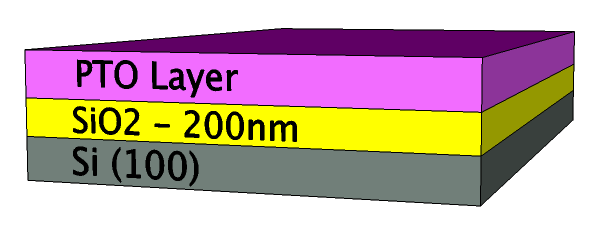
\includegraphics[width=0.75\textwidth]{./figures/DataAnalysis/ellipsometry-model-Si}
   \caption[Graphical Schematic of VASE Model]{A simple graphical example of the model used for %
   					analysis of the film stack in the Si(100) samples. The parameters %
					are $t$ and the spectroscopic values of $\tilde{n}$ for the PTO layer.}
   \label{fig:Si(100)-model}
\end{figure}

%%%%%%%%%%%%%%%%

\subsection{Analysis Procedure}
\label{chap:Methods-Ellip-Analysis}

Once the data was collected, a specific series of steps was followed in order to obtain the highest degree of accuracy from the model. All steps were performed on the PTO layer. The modeling procedure went as follows:

\begin{enumerate}
\item
High-$\lambda$ Cauchy Model
\item
Direct Calculation of $n$ and $\kappa$
\item
Conversion to Oscillator Model
\item
Refinement of Oscillator Layer Parameters
\end{enumerate}

This first step takes advantage of the transparency of the film at high wavelengths (low energies) where the photon energy is below the optical bandgap of the material. In this region, the Cauchy model can be used. The Cauchy model is empirical rather than physically descriptive, and best used for amorphous materials such as polymeric films, however the assumptions required for reasonable accuracy are met when absorption in the film layer is minimized (therefore $\kappa(\lambda)\approx0$). The equations used in the Cauchy model are shown in equation~\vref{eq:cauchy}. Generally, analysis during this step was performed in the spectral region where $\lambda = 600-1000$ nm ($E_{ph} = 2.06-1.24$ eV). 

\begin{subequations}
\label{eq:cauchy}
\begin{align}
	n\left(\lambda\right) &= A_{n} + \frac{B_{n}}{\lambda^{2}}+\frac{C_{n}}{\lambda^{4}}+\cdots\\
        	\kappa\left(\lambda\right) &= A_{\kappa}e^{B_{\kappa}\left(\frac{hc}{\lambda}\right)-C_{\kappa}}
\end{align}
\end{subequations}

Once reasonable estimates for $n$, $\kappa$, and the film layer thickness are obtained at the higher wavelengths, the second step of the analysis is to generate values of $\tilde{n}$ for the rest of the spectrum. The film thickness parameter is fixed at the value determined from the Cauchy model. The values of $n$ and $\kappa$ are allowed to be determined freely without the use of a model (i.e. directly determined by use of the Fresnel relations). This type of modeling is not physical, but assists in the generation of the oscillator-based model in the next step. The software package is then instructed to run a point-by-point fit of the data from highest- to lowest-$\lambda$, attempting to minimize the change in $n$ or $\kappa$ between adjacent data points. 

This model is then inputted into a oscillator model. For the analysis of these films, a Tauc-Lorentz oscillator model was utilized. The oscillator models used by WVASE32 are expressed in terms of the complex dielectric function $\tilde{\epsilon}$, which relates to $\tilde{n}$ via the relationship in equation~\vref{eq:dielectric}. The Tauc-Lorentz model changes the Lorentzian model by allowing for some absorption below the fundamental bandgap energy, which would be due to defect states and other intra-band transition mechanisms. The Tauc-Lorentz model uses the parameterization shown in equation~\vref{eq:TaucLorentz}\cite{WVASE-manual,Jellison96}. $\epsilon_{1}$ is provided here in a condensed version (eq.~\vref{eq:TaucLorentz-1}); the full expanded version, explanation of terms and variables, and the complete derivation via Kramers-Kronig consistent integration (whose relations are shown in equation \vref{eq:KK-relation})\cite{Jellison96,KRONIG:26,PhysRev.104.1760} from $\epsilon_{2}$, has been presented by Jellison and Modine.\cite{Jellison96} 

\begin{subequations}
\label{eq:dielectric}
\begin{align}
	\tilde{\epsilon} &= \epsilon_{1}+i\epsilon_{2} = \tilde{n}^{2}\\
	\epsilon_{1} &= n^{2} - \kappa^{2}\\
	\epsilon_{2} &= 2n\kappa 
\end{align}
\end{subequations}

\begin{subequations}
\label{eq:TaucLorentz}
\begin{align}
	\label{eq:TaucLorentz-1}
	\epsilon_{1}=\frac{2}{\pi}P\int^{\infty}_{E_{g}}\frac{\xi\epsilon_{2}\left(\xi\right)}{\xi^{2}-E^{2}}\,%
				\mathrm{d}\xi & \hspace{2.5cm}
\end{align}
\begin{empheq}[left=\empheqlbrace]{align}
	\epsilon_{2} (E) = \frac{AE_{0}C\left(E-E_{g}\right)^{2}}{\left(E^{2}-E^{2}_{0}\right)^{2}+C^{2}E^{2}}%
		\cdot \frac{1}{E} && E> E_{g}\\
        	\epsilon_{2} (E) = 0 && E\leq E_{g}
\end{empheq}
\end{subequations}\\

\begin{subequations}
\label{eq:KK-relation}
\begin{align}
	\epsilon_{1}\left(\omega\right)-1&=\frac{2}{\pi}P\int^{\infty}_{0}\frac{\omega^{\prime}\epsilon_{2}\left(\omega^{\prime}\right)}{\omega^{\prime2}-\omega^{2}}d\omega^{\prime}\\
	\epsilon_{2}\left(\omega\right)&=-\frac{2\omega}{\pi}P\int^{\infty}_{0}\frac{\epsilon_{1}\left(\omega^{\prime}\right)-1}{\omega^{\prime2}-\omega^{2}}d\omega^{\prime}
\end{align}
\end{subequations}

\indent The WVASE32 software package allows one to use a graphical interface to provide initial guesses for the various fit parameters. At times this required multiple oscillators to best fit the predicted $\epsilon_{2}$ function. Once this has been set, all of the parameters affecting $\epsilon_{2}$ ($A, E_{0}, C, E_{G}$) are marked to be included in the fit. The software is then instructed to perform a best-fit of the oscillator to $\epsilon_{2}$. Once this operation completes, the software is set to fit to $\epsilon_{1}$ and only the value of the $\epsilon_{1}$ offset is allowed to be fit. Finally, the software is set to optimize vs both $\epsilon_{1}$ and $\epsilon_{2}$, and all parameters are included. This completes the initial setup of the oscillator model. 

Finally, the model is set to also allow the layer thickness to be fit and a general fit to the entire experimental dataset is performed. This provides the best guess to the physical values of the film. The thickness calculated by this procedure matches very closely to measurements performed by other methods (e.g. SEM imaging or AFM measurement of a lithographically created step). 

If similar deposition parameters are utilized, it is possible to save the parameterized model for later use. This allows the analysis to be streamlined when the material is expected to remain constant, for example if tests of deposition at different layer thicknesses are performed. In this case, the material would have optical behavior very similar to the initial sample, and the oscillator model would be sufficiently close to valid parameters to be used directly for fits. All that would need to be adjusted initially would be the estimated layer thickness. If the fit fails to produce useful data, such as unreasonable values for any of the parameters or very large confidence intervals, it is recommended to proceed with the entire standard analysis procedure. 

Further analysis can be performed to estimate the bandgap of the layer, via Tauc plot analysis.\cite{tauc_optical_1968,ablees_optical_1972,Bruzzese_2010} The method requires the calculation of the absorption coefficient ($\alpha$) from the value of $k$ for the layer (see equation~\vref{eq:alpha}). $\alpha$ is usually provided in terms of cm$^{-1}$, so if the wavelength is provided in nanometers a corresponding factor of $10^{7}$ must be incorporated as well. Subsequently, a Tauc plot is constructed using a combination of $\alpha$ and the photon energy. For direct bandgap materials the Tauc parameter is given by $\left(\alpha E_{ph}\right)^{2}$.\cite{tauc_optical_1968,ablees_optical_1972,Bruzzese_2010} If the bandgap is of the indirect type, the function is changed to $\sqrt{\alpha E_{ph}}$. The bandgap parameter matches well to literature values (when using standard samples of well defined materials, such as a thin layer of titania). It must be noted that the bandgap that is calculated is the overall bandgap of the layer, which may be a combination of multiple phases or materials.\cite{tauc_optical_1968,ablees_optical_1972,Bruzzese_2010}

\begin{equation}
	\label{eq:alpha}%
	\alpha = \frac{4\pi k}{\lambda}
\end{equation}

Experimental data sets, the resulting fitted models, and Tauc analyses for selected samples are presented in appendix~\vref{sup:Ellipsometry}.

%%%%%%%%%%%%%%%%%%%%%%%%%%%%%%%%%%%%%%%%%%%%%%%%%%%%
%%%%%%%%%%%%%%%%%%%%%%%%%%%%%%%%%%%%%%%%%%%%%%%%%%%%
%%%%%%%%%%%%%%%%%%%%%%%%%%%%%%%%%%%%%%%%%%%%%%%%%%%%

\section{Composition Analysis}
\label{sec:Methods-Comp}

In order to crystallize the film into a desired phase, without having additional impurity phases form, it is important to be able to control the stoichiometry of the produced film. Previous reports have shown that there is a close relationship between the composition of the film and the final resultant phase (see figure~\vref{fig:PTO-phase}).\cite{harjuoja_2006} 

\begin{figure}[tb]
   \centering
   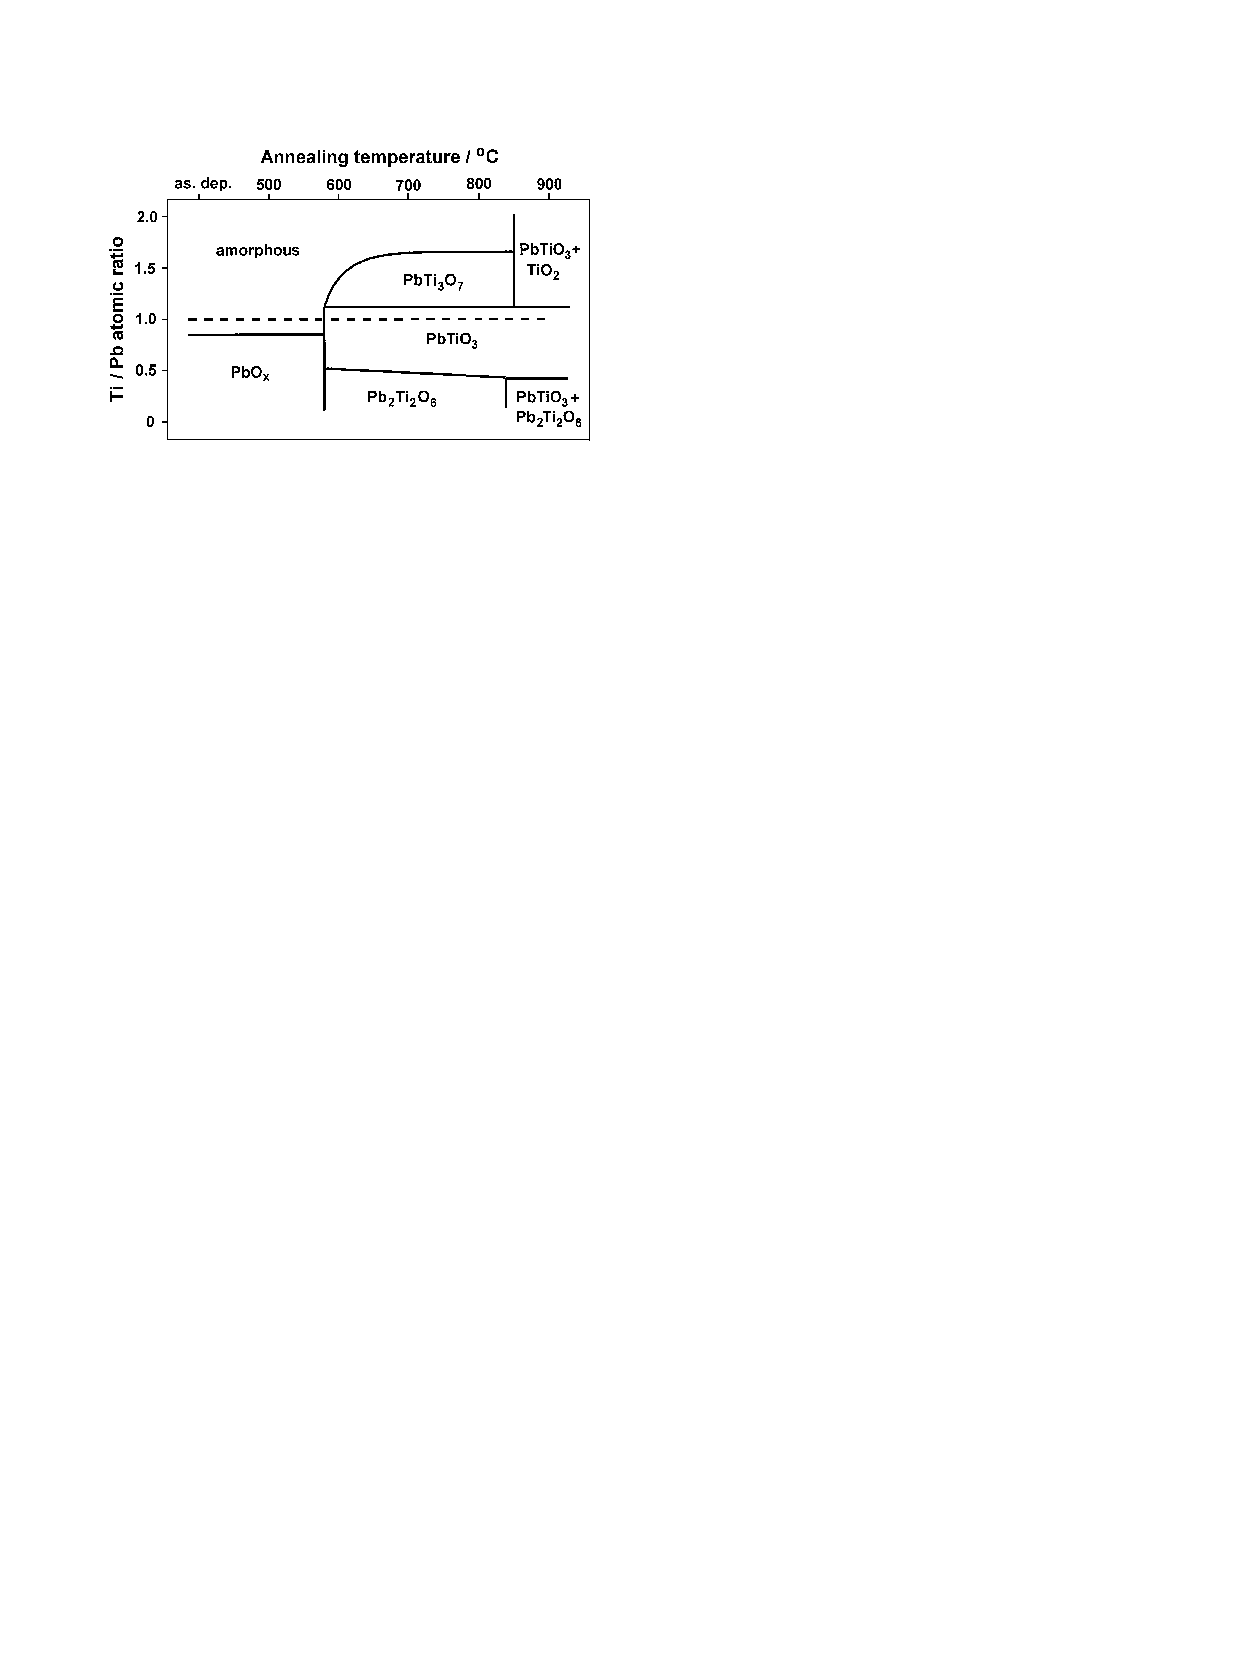
\includegraphics[width=0.75\textwidth]{./figures/dataanalysis/PTO-phase}
   \caption[Preferred Phase vs. Stoichiometric Ratio]{Graphic illustrating preferred phase of an annealed %
   		film at a range of stoichiometric ratios and annealing temperatures. A slight excess of \ce{Pb} %
		in the system is expected to help stabilize the perovskite \PTO{} phase.\cite{harjuoja_2006}\\
		{\tiny Image reprinted with permission from the Publisher.}}
   \label{fig:PTO-phase}
\end{figure}

\lipsum

%%%%%%%%%%%%%%%%

\subsection{X-Ray Fluorescence Spectroscopy}
\label{sec:Methods-XRF}

X-ray Fluorescence was the primary method used for determining the composition of the deposited films. Analysis was performed in a scanning electron microscope (FEI Strata DB235). The sample was imaged in order to identify the exact height of the sample within the chamber, via the microscope's focal length. After the sample had been properly positioned, the imaging beam was disengaged and the X-ray source activated. Then, in much the same manner as EDS, the emitted X-rays are collected and analyzed. A target X-ray count was around 20,000-50,000 for most samples. If the film on a particular sample was found to be very thin, more counts were often required to obtain well-defined peaks for the film elements. 

Initial calibration of the system is critically important to acquiring accurate measurements. Calibration is performed using a pair of standard samples of known composition, which include all elements that are to be quantified. For this study, a pellet of commercially prepared \PTO{} powder and a thin film of \ce{PbZr_{0.52}Ti_{0.48}O3} were used as standards. 

The only major issue with XRF --- and composition analysis in general --- that was encountered during the course of this work was the fact that it was not surface sensitive. In fact, many of the observed counts could be attributed to the substrate. In general this proved not to be problematic, but when the sample and film had elements in common this analysis was confounded and completely impossible to perform using XRF. This was the case with PTO films deposited on \ce{SrTiO3} substrates, as both the film and the substrate had titanium content. 

This issue could have been circumvented by using surface-sensitive techniques; examples of these methods include Auger electron spectroscopy (AES), X-ray photoelectron spectroscopy (XPS), and Rutherford backscattering spectroscopy (RBS). Unfortunately, none of these tools were available at the time and as such samples deposited on STO do not have associated composition information. 

%%%%%%%%%%%%%%%%%%%%%%%%%%%%%%%%%%%%%%%%%%%%%%%%%%%%
%%%%%%%%%%%%%%%%%%%%%%%%%%%%%%%%%%%%%%%%%%%%%%%%%%%%
%%%%%%%%%%%%%%%%%%%%%%%%%%%%%%%%%%%%%%%%%%%%%%%%%%%%

\section{X-Ray Diffraction}
\label{sec:Methods-XRD}

X-ray diffraction (XRD) was used in this study to investigate the phases that crystallized in the samples after annealing treatments were performed.  Sample alignment was an automated, preprogrammed process for film-type structures; the system performed alignments on all available axes to ensure optimum sample placement and orientation. Calibration of the system was managed by lab technicians. 

Data was collected in the standard $\theta-2\theta$ orientation, and was programmed to sweep ranges between 10--90$^{\circ}$. Varying time constants were used on different samples, as samples with thicker ALD films supplied a stronger signal. 

%%%%%%%%%%%%%%%%

%\subsection{Grazing Incidence XRD}
%
%For each sample, the value of $\omega$ was set to be 80\% of the film's critical angle which was determined prior to the scan. 






\chapter{Results}
\label{ch:Results}
\thispagestyle{empty}

%%%%%%%%%%%%%%%%%%%%%%%%%%%%%%%%%%%%%%%%%%%%%%%%%%%%%%%%%%
%%%%%%%%%%%%%%%%%%%%%%%%%%%%%%%%%%%%%%%%%%%%%%%%%%%%%%%%%%
%%%%%%%%%%%%%%%%%%%%%%%%%%%%%%%%%%%%%%%%%%%%%%%%%%%%%%%%%%

As discussed, the goal of this study was to determine methods for atomic layer deposition of ferroelectric oxides. In the process of realizing this goal there were a number of different areas of study. The first is the analysis of thermal and chemical behavior of the various potential precursors, during which TGA and DSC were primarily used (see~\vref{sec:Methods-Thermal}). Secondly,  the analysis of the film growth behavior under various conditions, this was primarily measured and analyzed using the ellipsometric techniques discussed earlier (see~\vref{sec:Methods-Ellip}). Third, the film deposition needed to be tuned to produce films with a stoichiometric composition, as this was expected to produce films which would crystallize into the desired perovskite phase, see Section~\vref{sec:Methods-Comp} for the methods used for this characterization. Fourth, the phase of the crystallized film was analyzed in detail to determine behavior of the films post-annealing. XRD was used extensively for this task (see~\vref{sec:Methods-XRD}).


%%%%%%%%%%%%%%%%%%%%%%%%%%%%%%%%%%%%%%%%%%%%%%%%%%%%%%%%%%
%%%%%%%%%%%%%%%%%%%%%%%%%%%%%%%%%%%%%%%%%%%%%%%%%%%%%%%%%%
%%%%%%%%%%%%%%%%%%%%%%%%%%%%%%%%%%%%%%%%%%%%%%%%%%%%%%%%%%

\section{Thermal Analysis}
\label{chap:Results-Thermal}

While a viable titanium precursor was well identified in literature as well as experimentally, as was the oxidizers that were used, there was no such universally accepted chemical used in ALD to provide a source of lead. The primary issue was either a lack of chemical stability or a undesirably low volatility in the compounds that currently were being used. TGA and DSC was performed on a number of potential candidates (see~\vref{sec:SampFab-Precursors} for more details) in order to gauge the performance of these materials. 

%%%%%%%%%%%%%%%%

\subsection{Thermogravimetric Analysis}

Thermogravimetric analysis allows for the estimation and comparison of volatility between multiple samples. It was used in this study primarily to compare properties of the two candidate precursors, \HFAc{} and \TMHD{}. Of primary consideration was the volatility of the compound --- evaluated qualitatively by analyzing the mass loss at various temperatures --- and whether or not there are indications of imperfect evaporation. The data collected for these materials can be found below. 

By analyzing the TGA curve for \HFAc{}, found in figure~\vref{fig:TGA-HFAc-Weight}, there are a number of features that are immediately noticeable. First of these is the presence of multiple stages of evaporation in the curve. These occur at approximately 170 and 190\degC{}. A TGA curve for a material that is purely evaporative, e.g. pure water, will have a smooth curve. Additional steps indicate that other processes are activating, and causing changes to the compound affecting the mass loss. 

More detail can be seen by performing a derivation on the TGA curve, giving the mass loss rate. This plot can be found in figure~\vref{fig:TGA-HFAc-DWeight}. This plot shows a shoulder on the primary evaporative peak, and then another peak starting at around 170\degC{} and peaking at 190\degC{}. The shoulder indicates that even during the evaporation of the bulk of the material, before residues and other imperfections cause rate changes, a secondary mechanism is activating and impacting the mass loss rate. 

\begin{figure}[tbp]
   \centering
   \subfloat[Mass vs. Temperature][Mass vs. Temperature]{%
   	\label{fig:TGA-HFAc-Weight}%
	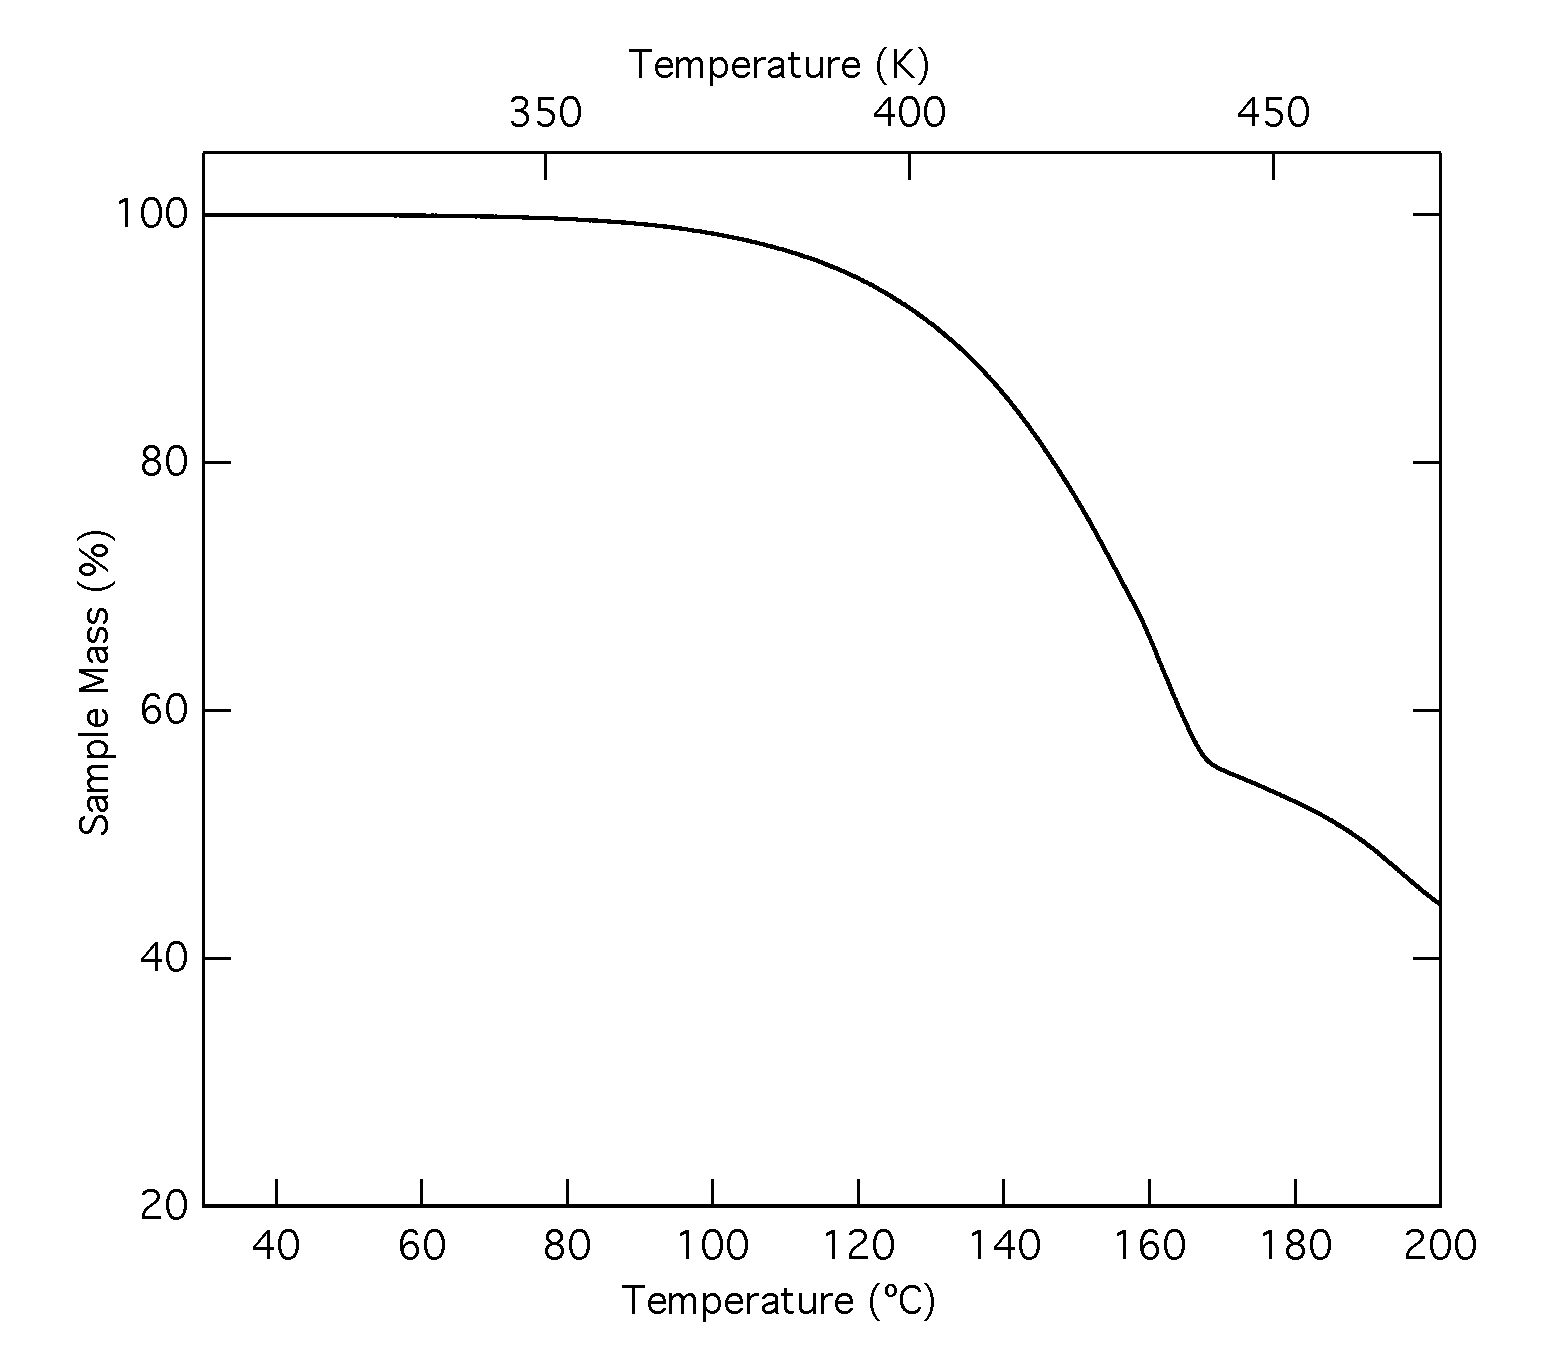
\includegraphics[width=0.45\textwidth]{./Figures/Data/Thermal-Analysis/TGA/HFAc-Weight}%
	}
	\hspace{1cm}
  \subfloat[Derivative of Mass vs. Temperature][Derivative of Mass vs. Temperature]{%
   	\label{fig:TGA-HFAc-DWeight}%
	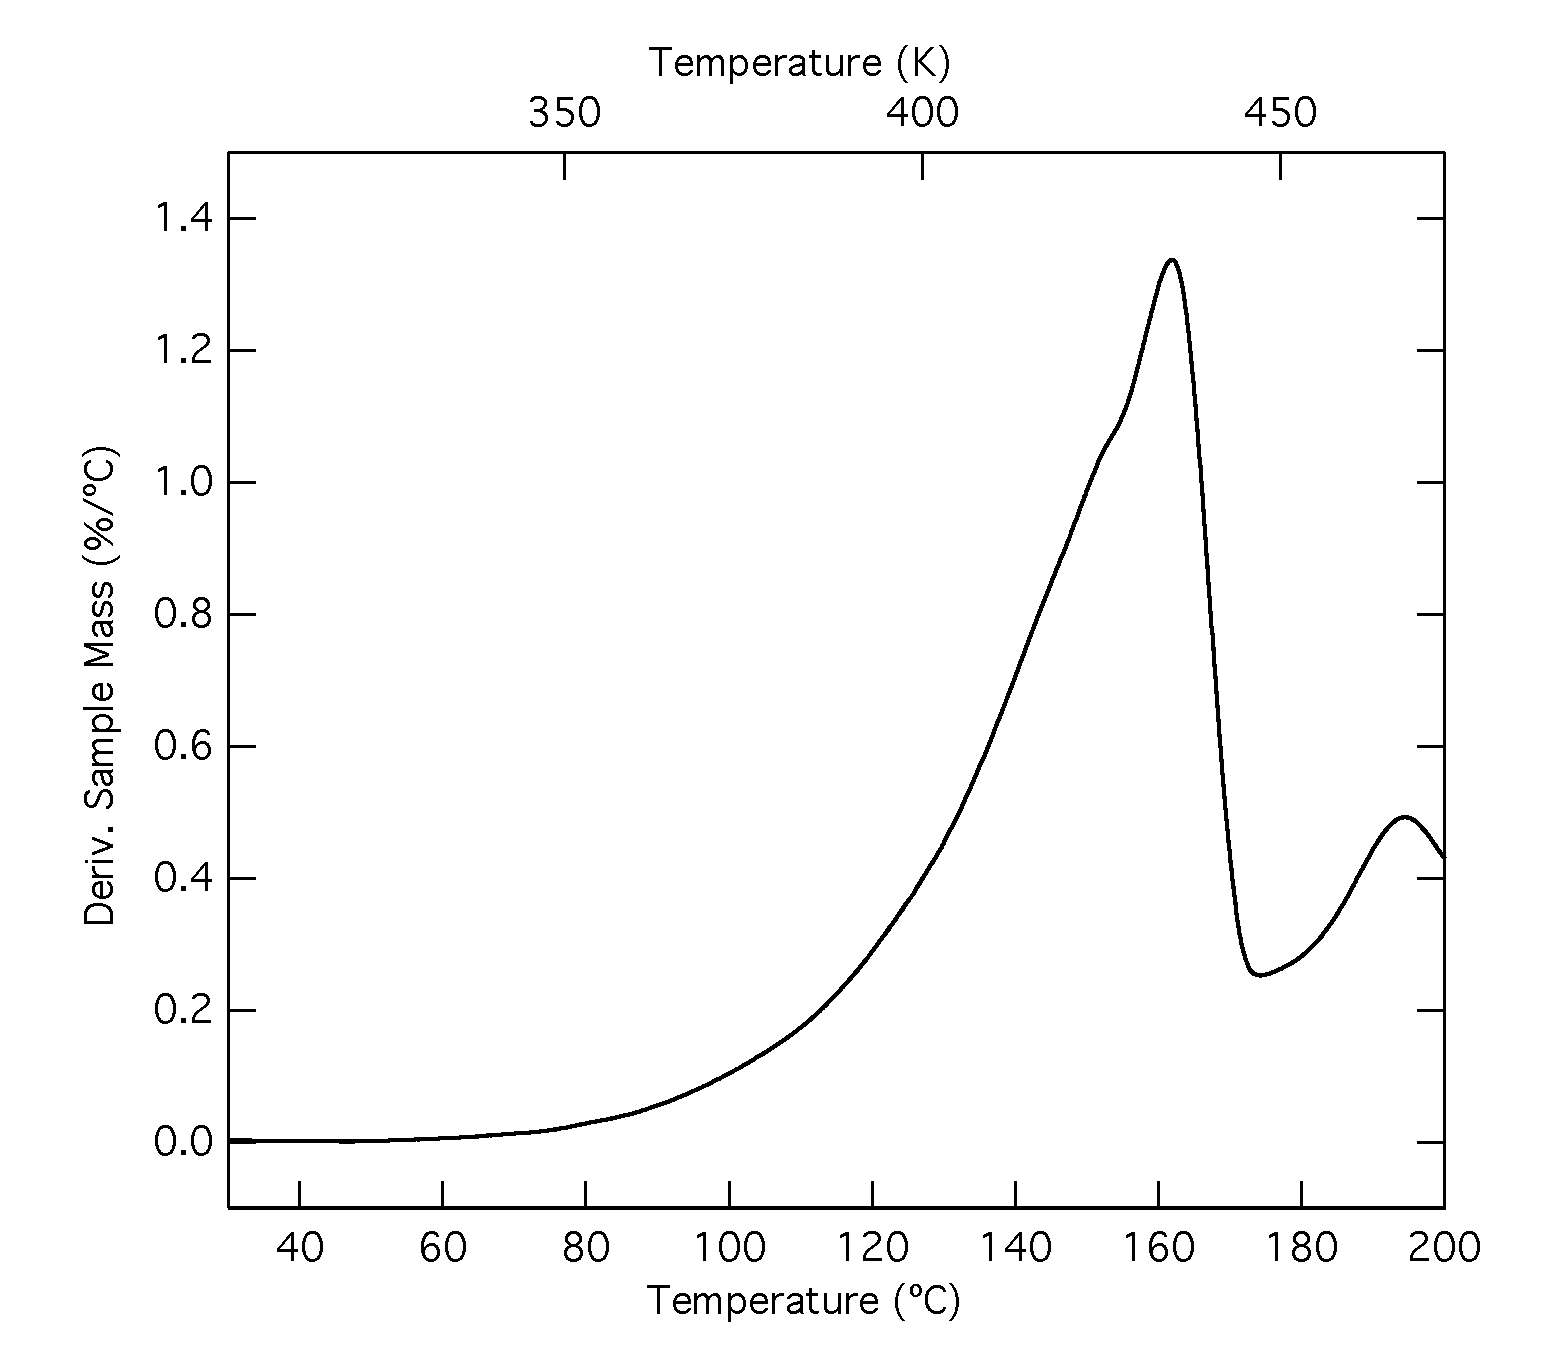
\includegraphics[width=0.45\textwidth]{./Figures/Data/Thermal-Analysis/TGA/HFAc-DWeight}%
	} 	
   \caption[TGA Results for Pb(HFAc)$_{2}$ Precursor]%
   		{Plots of the results from TGA experiments on Pb(HFAc)$_{2}$. The plot shown in (a) gives the raw %
		data showing the current mass as a function of temperature. (b) gives the same data, transformed %
		to show the derivative of mass. Thus (b) shows the rate of mass loss at a given temperature. Initial %
		sample mass: 6.092 mg}
   \label{fig:TGA-HFAc}
\end{figure}

Comparing this data with that of \TMHD{}, it is immediately obvious that the evaporation mechanism for the latter is much smoother. There is no major visible step, apart from some slight changes nearing the upper end of the testing temperature range (185--200\degC{}). With a closer look at figure~\ref{fig:TGA-TMHD-DWeight}, it is easier to see that there is smooth vaporization up to approximately 180\degC{}, at which point the evaporation is slowed dramatically due to residue buildup. 

\begin{figure}[tbp]
   \centering
   \subfloat[Mass vs. Temperature][Mass vs. Temperature]{%
   	\label{fig:TGA-TMHD-Weight}%
	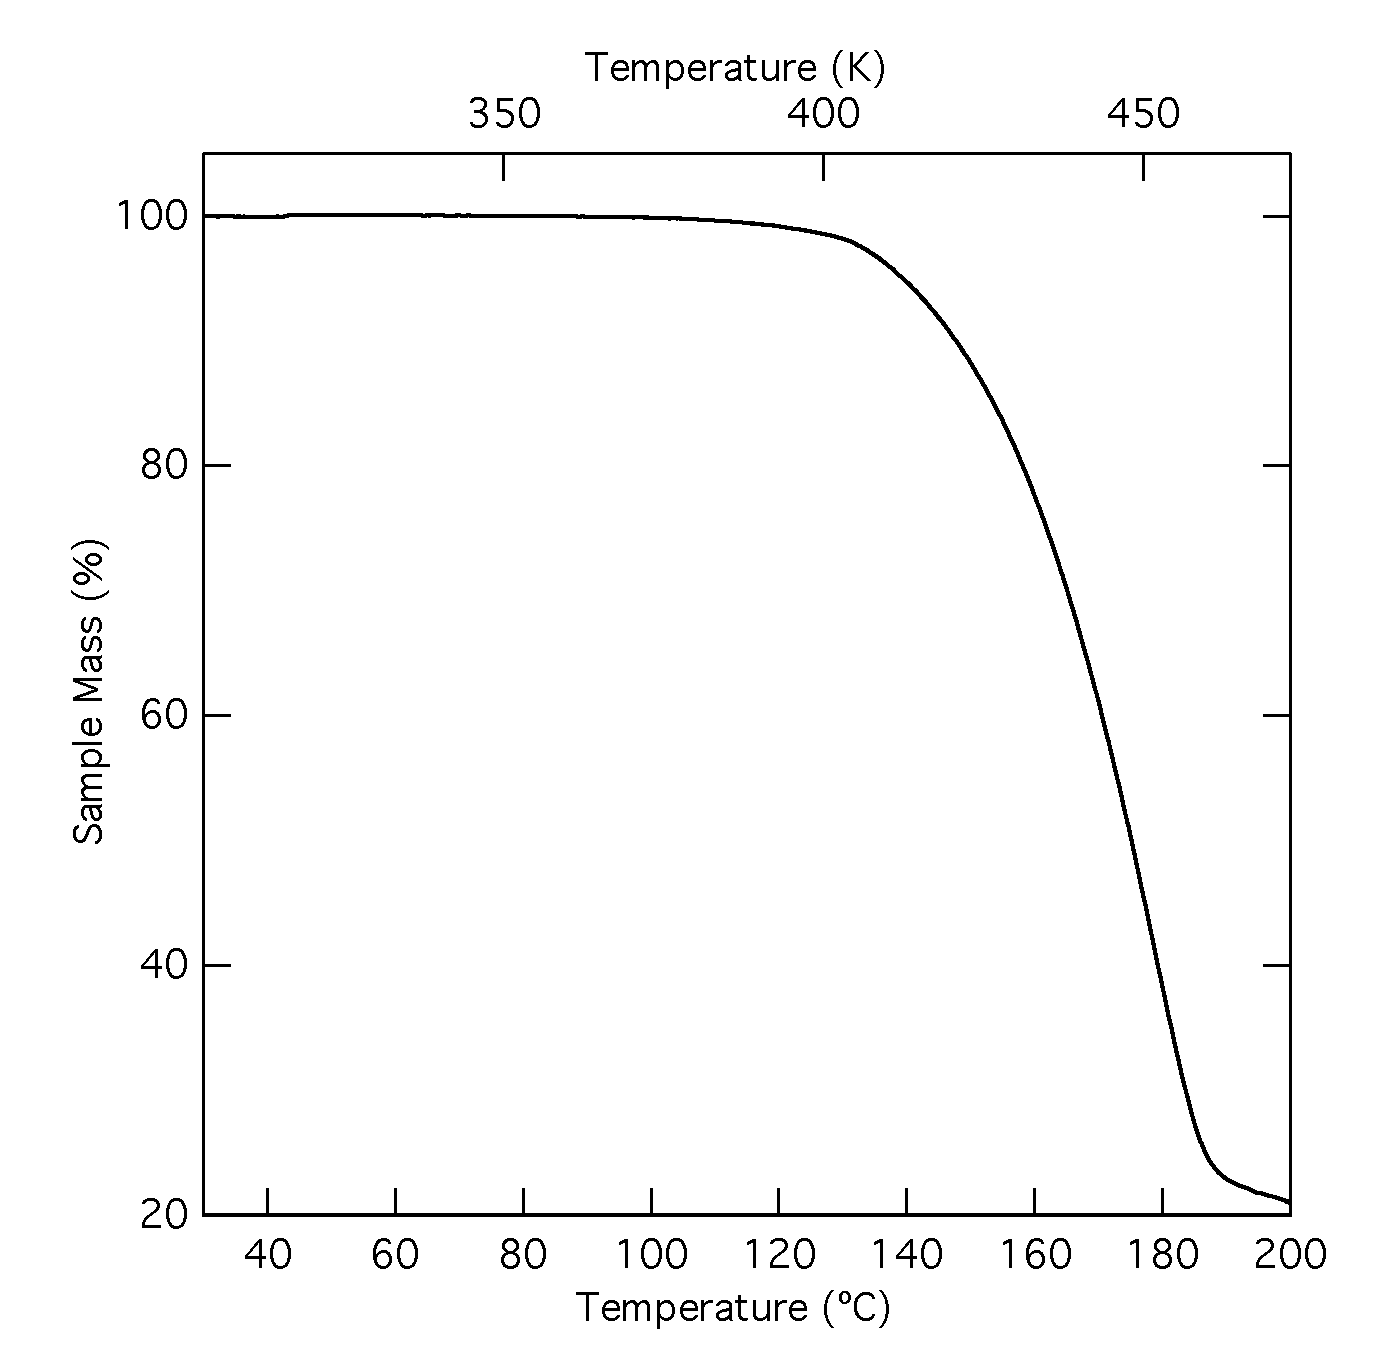
\includegraphics[width=0.45\textwidth]{./Figures/Data/Thermal-Analysis/TGA/TMHD-Weight}%
	}
	\hspace{1cm}
  \subfloat[Derivative of Mass vs. Temperature][Derivative of Mass vs. Temperature]{%
   	\label{fig:TGA-TMHD-DWeight}%
	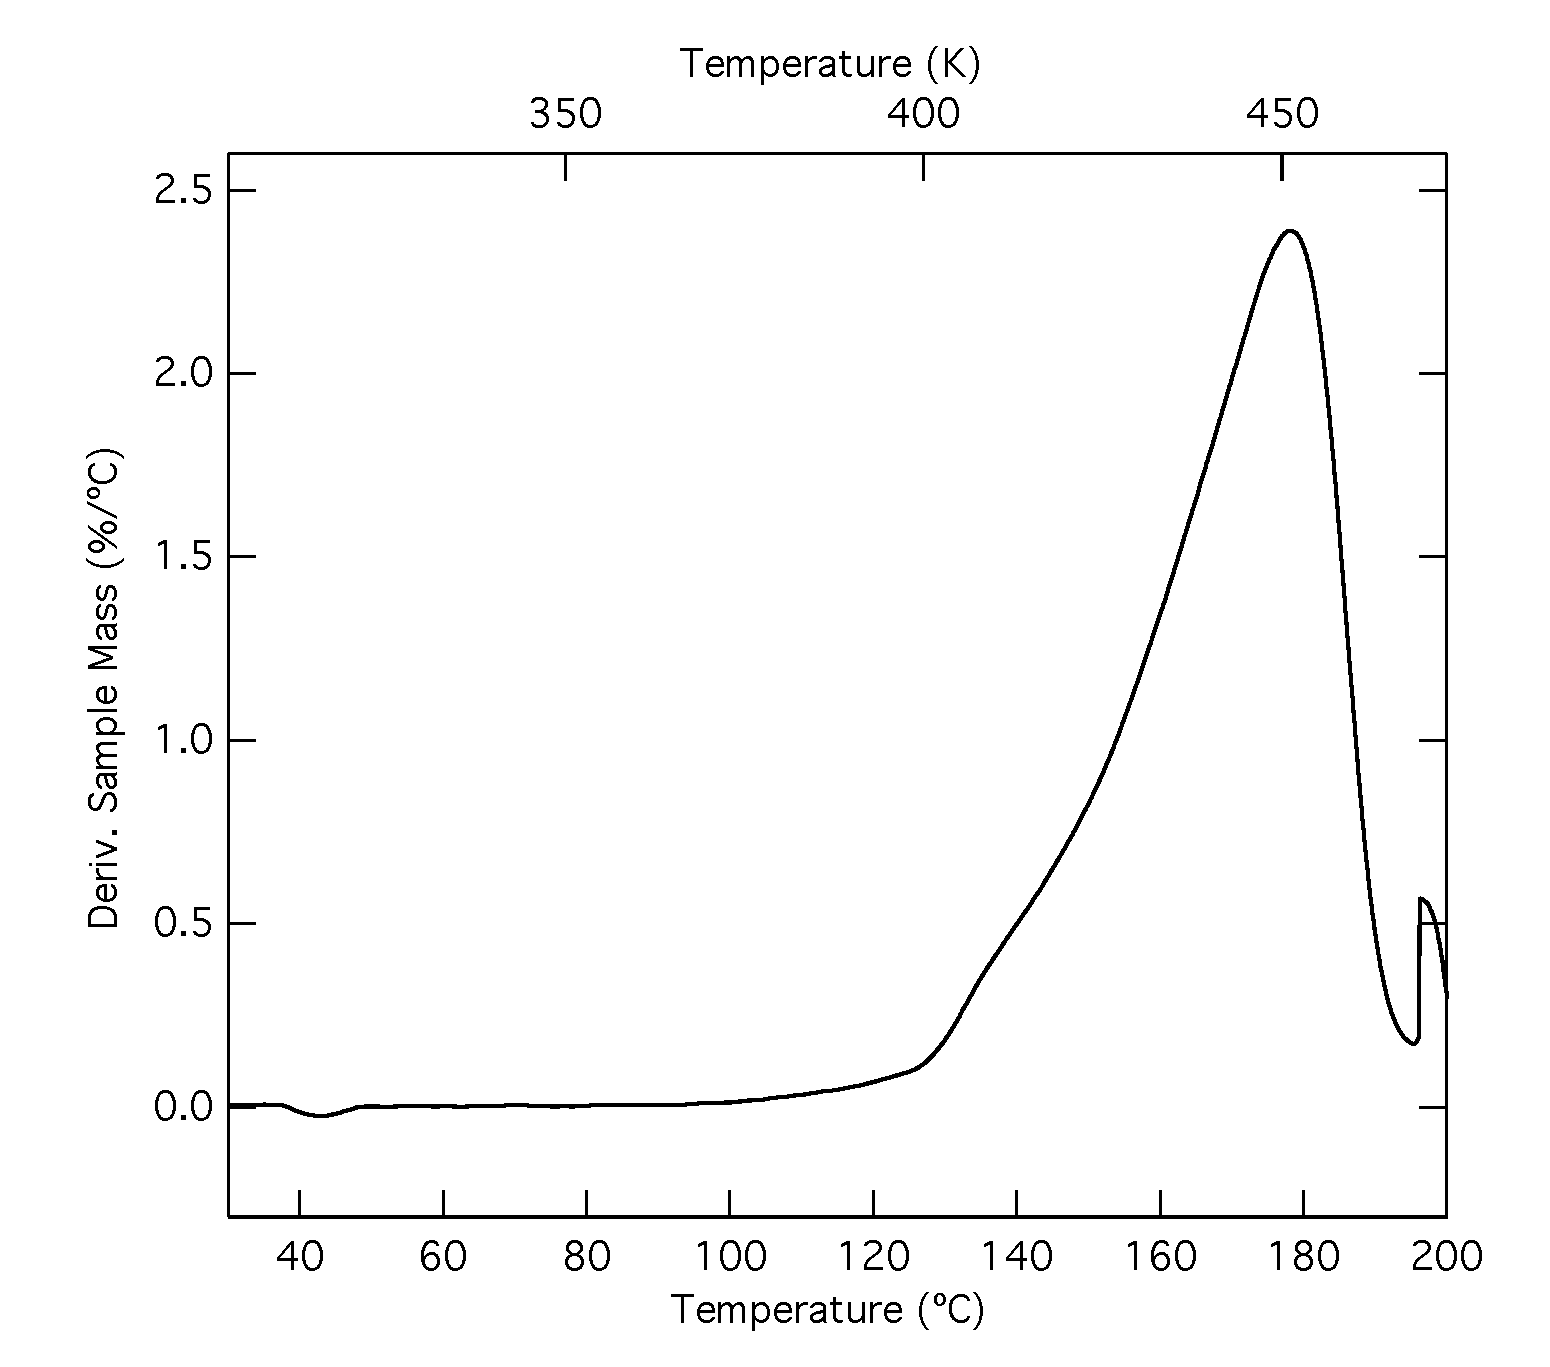
\includegraphics[width=0.45\textwidth]{./Figures/Data/Thermal-Analysis/TGA/TMHD-DWeight}%
	} 	
   \caption[TGA Results for Pb(HFAc)$_{2}$ Precursor]%
   		{Plots of the results from TGA experiments on Pb(TMHD)$_{2}$. As in figure~\vref{fig:TGA-HFAc}, (a) %
		presents the actual mass as a function of temperature, while (b) gives the derivative of that function. %
		Initial sample mass: 3.719 mg}
   \label{fig:TGA-TMHD}
\end{figure}

Neither of these precursors evaporated cleanly, leaving residues of more than 20\% of their initial sample mass during the temperature scanning tests discussed above. When these were tested at moderate temperatures, such as those to be used for evaporation in the ALD system, both left even larger fractions of their initial masses behind. Testing at a constant temperature (160\degC{}) over a longer period of time gives the plots shown in figure~\vref{fig:TGA-Hold}. From this test, it was found that \HFAc{} left a much larger residue than \TMHD{}, 63\% and 34\% respectively. 

\begin{figure}[tbp]
   \centering
   \subfloat[\HFAc][\HFAc]{%
   	\label{fig:TGA-HFAc-Hold}%
	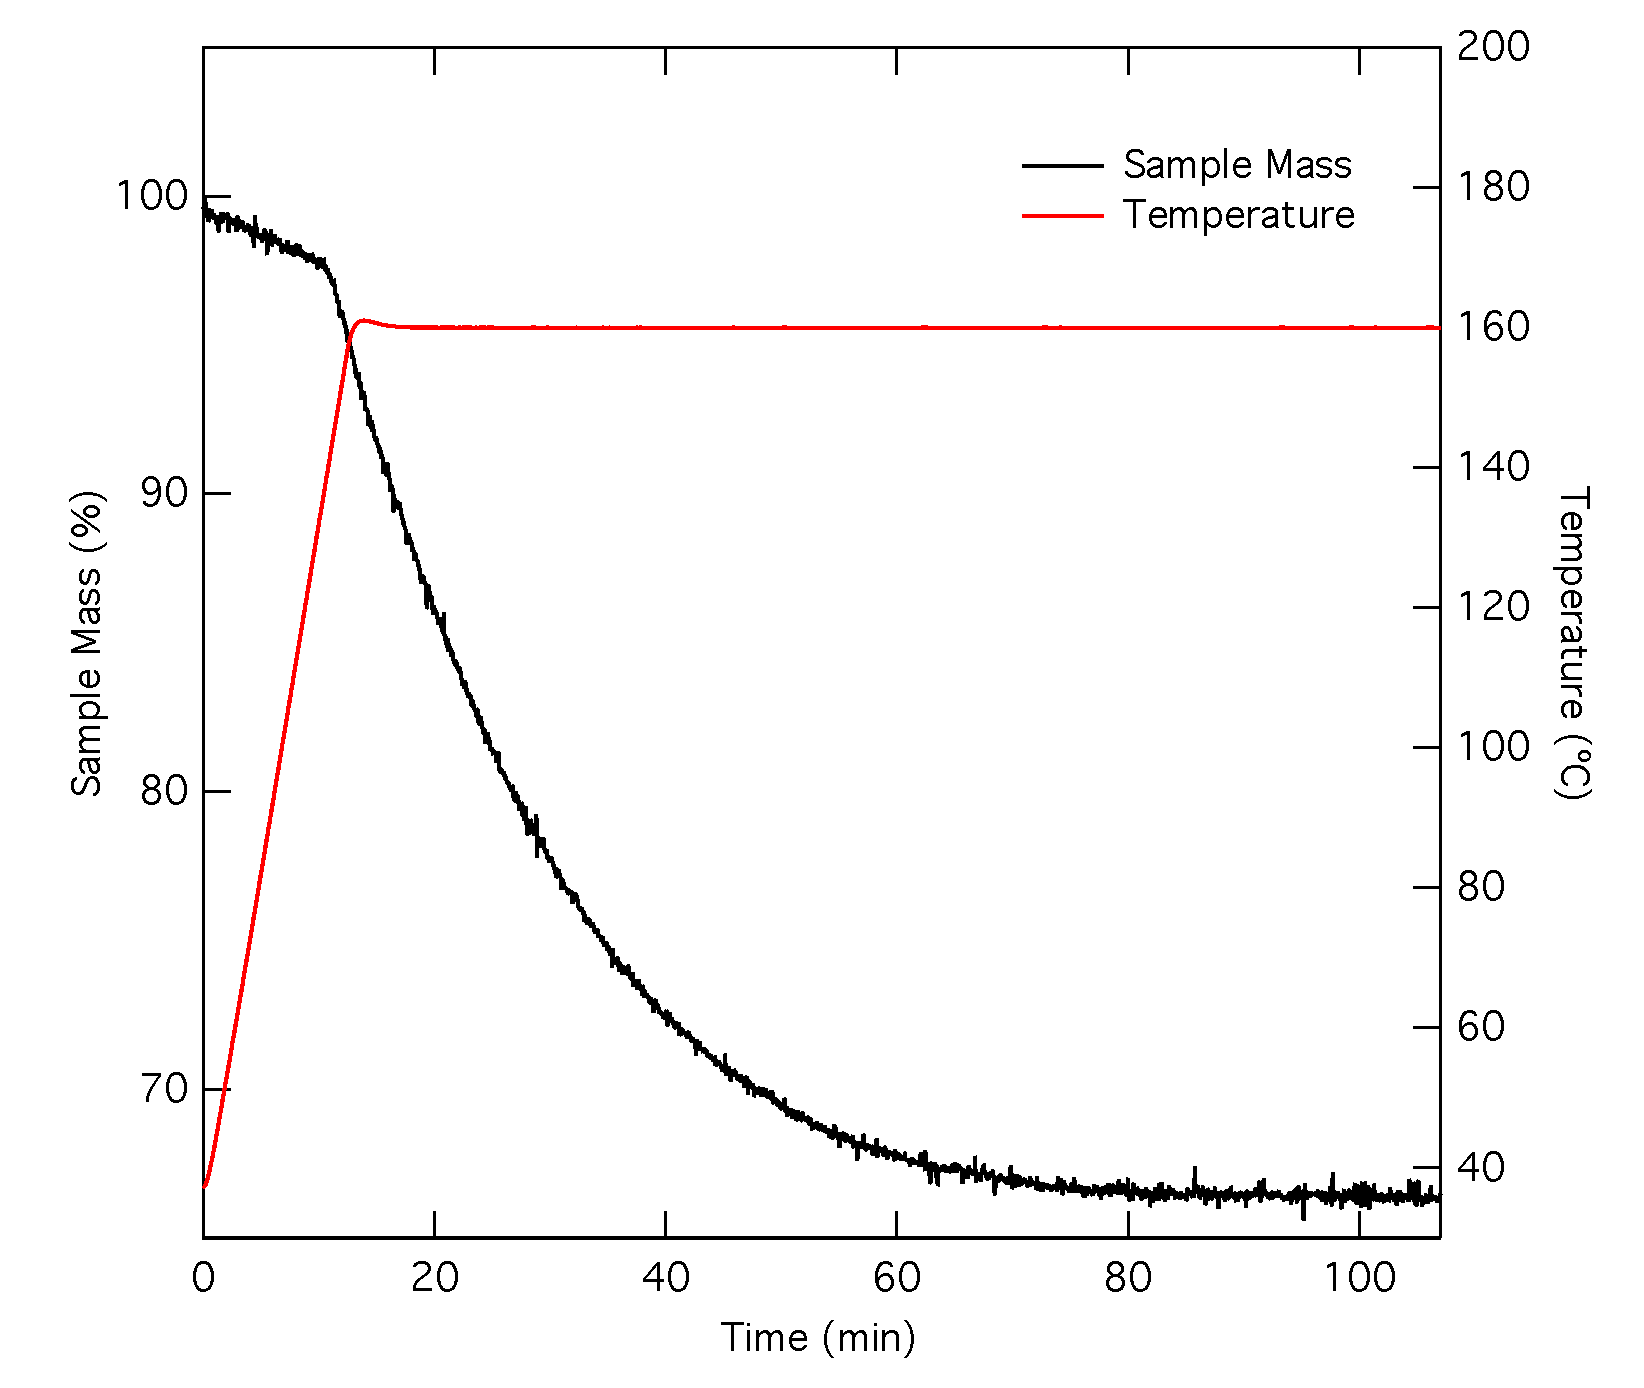
\includegraphics[width=0.45\textwidth]{./Figures/Data/Thermal-Analysis/TGA/HFAc-Hold}%
	}
	\hspace{1cm}
  \subfloat[\TMHD][\TMHD]{%
   	\label{fig:TGA-TMHD-Hold}%
	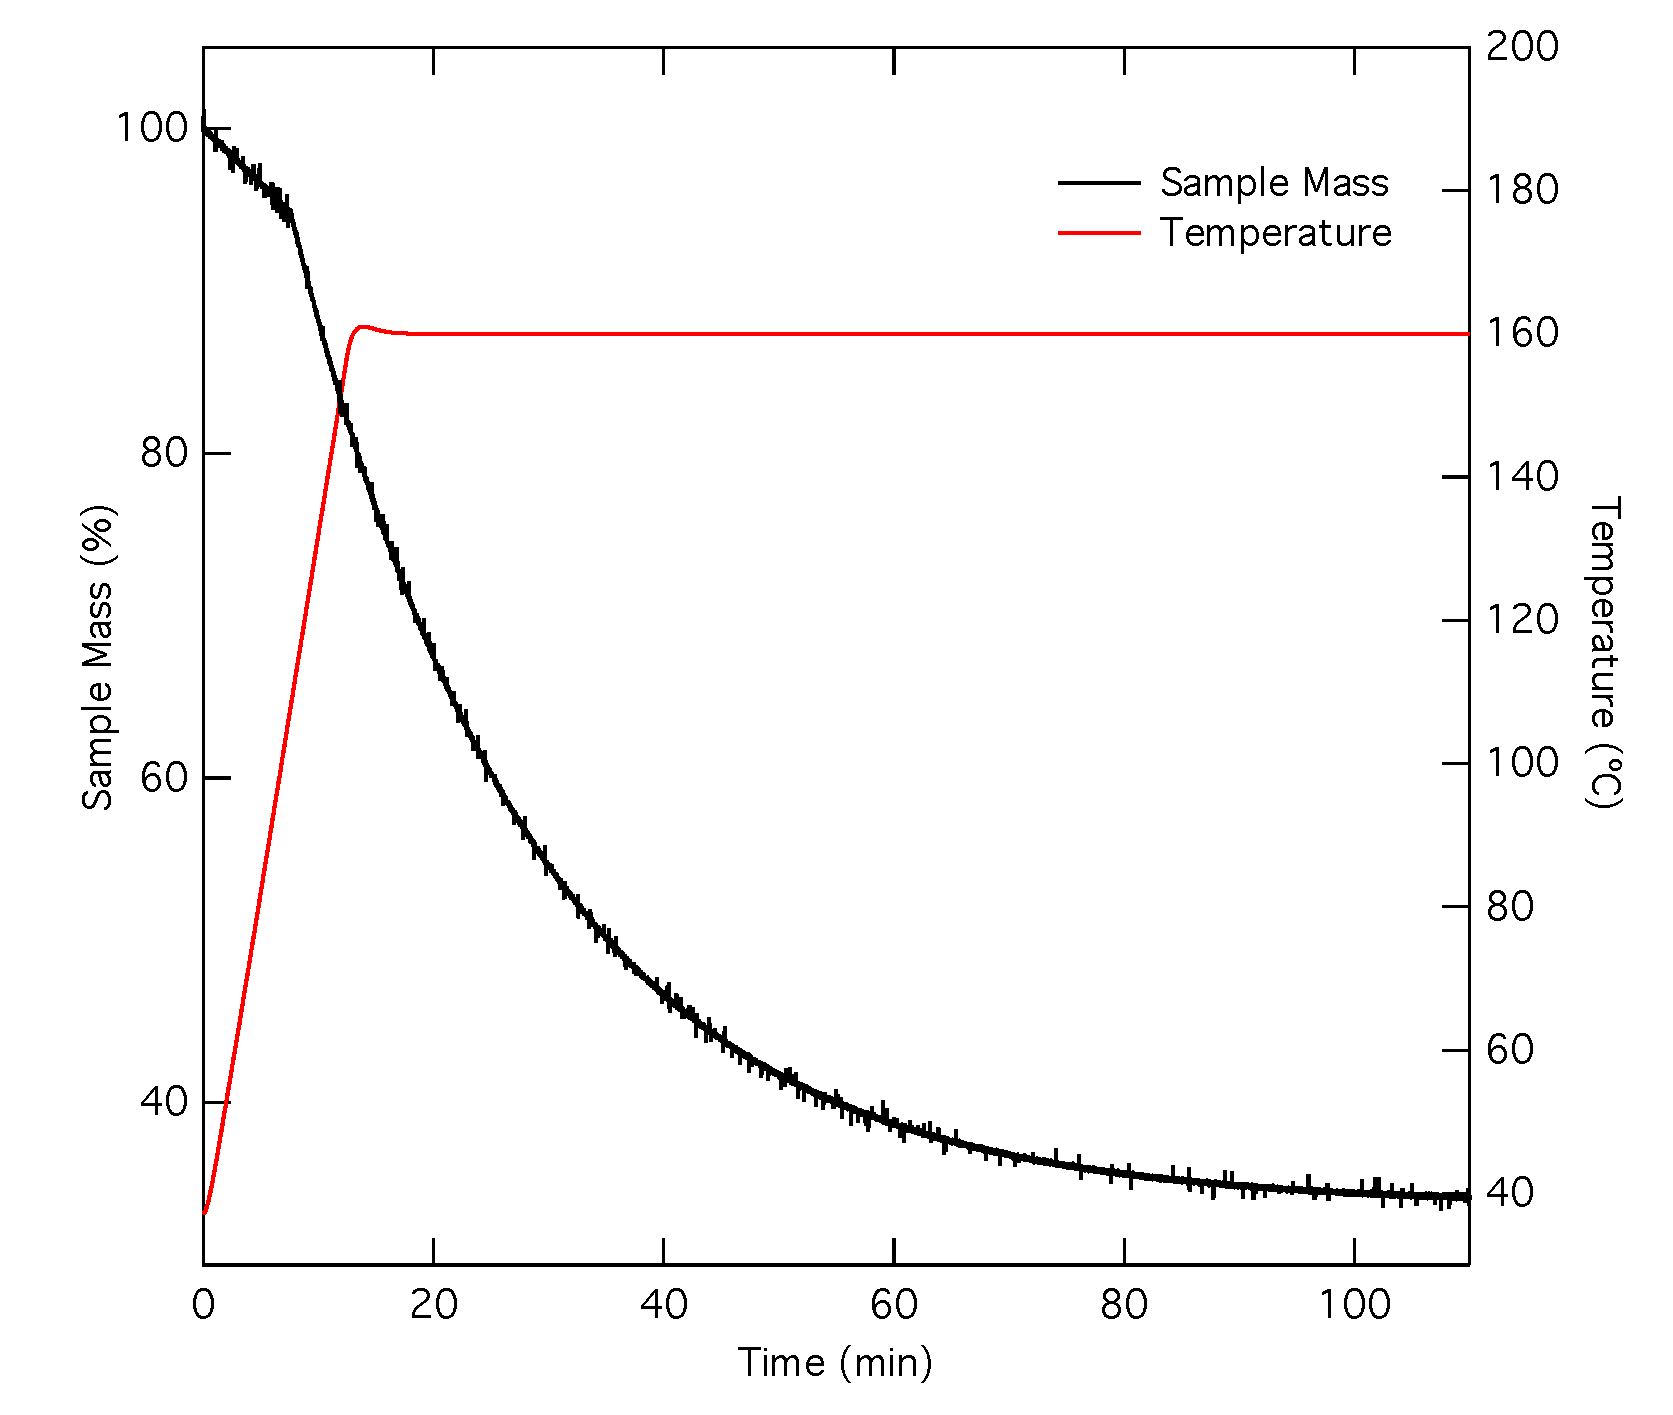
\includegraphics[width=0.45\textwidth]{./Figures/Data/Thermal-Analysis/TGA/TMHD-Hold}%
	} 	
   \caption[Constant Temperature TGA Experiments]%
   		{Plots of the results from ramp-and-hold TGA experiments designed to investigate residual material %
		after complete evaporation at a given temperature. From the TGA experiments seen above (figs.~%
		\vref{fig:TGA-HFAc} and \vref{fig:TGA-TMHD}), a common temperature of 160\degC{} was chosen %
		for this experiment. Sample masses were 3.921 mg and 4.381 mg for \HFAc{} and \TMHD{} respectively.}
   \label{fig:TGA-Hold}
\end{figure}

Based on the results of these tests, the lower residual mass and the cleaner evaporative process, \TMHD{} was predicted to have better performance as an ALD precursor. 

%%%%%%%%%%%%%%%%

\subsection{Differential Scanning Calorimetry}

As discussed in previous chapters, DSC is a powerful tool for analyzing the behavior of precursors. The data collected allows for the understanding of various energies in the material. 

When considering the energetic behavior of \HFAc{} (see fig.~\vref{fig:DSC-HFAc}), there are a few minor features that can be noticed. Primarily at 25 and 150\degC{} small peaks are visible that indicate changes in the material other than the solid to liquid phase change, which is the much larger peak seen around 155-160\degC{}. However, these peaks appear to be negligible, as the total energy release by the sample is a mere 5.32 mJ (1.13 J/g), which is too low for any major chemical changes to be occurring. 

\begin{figure}[htb]
	\centering
	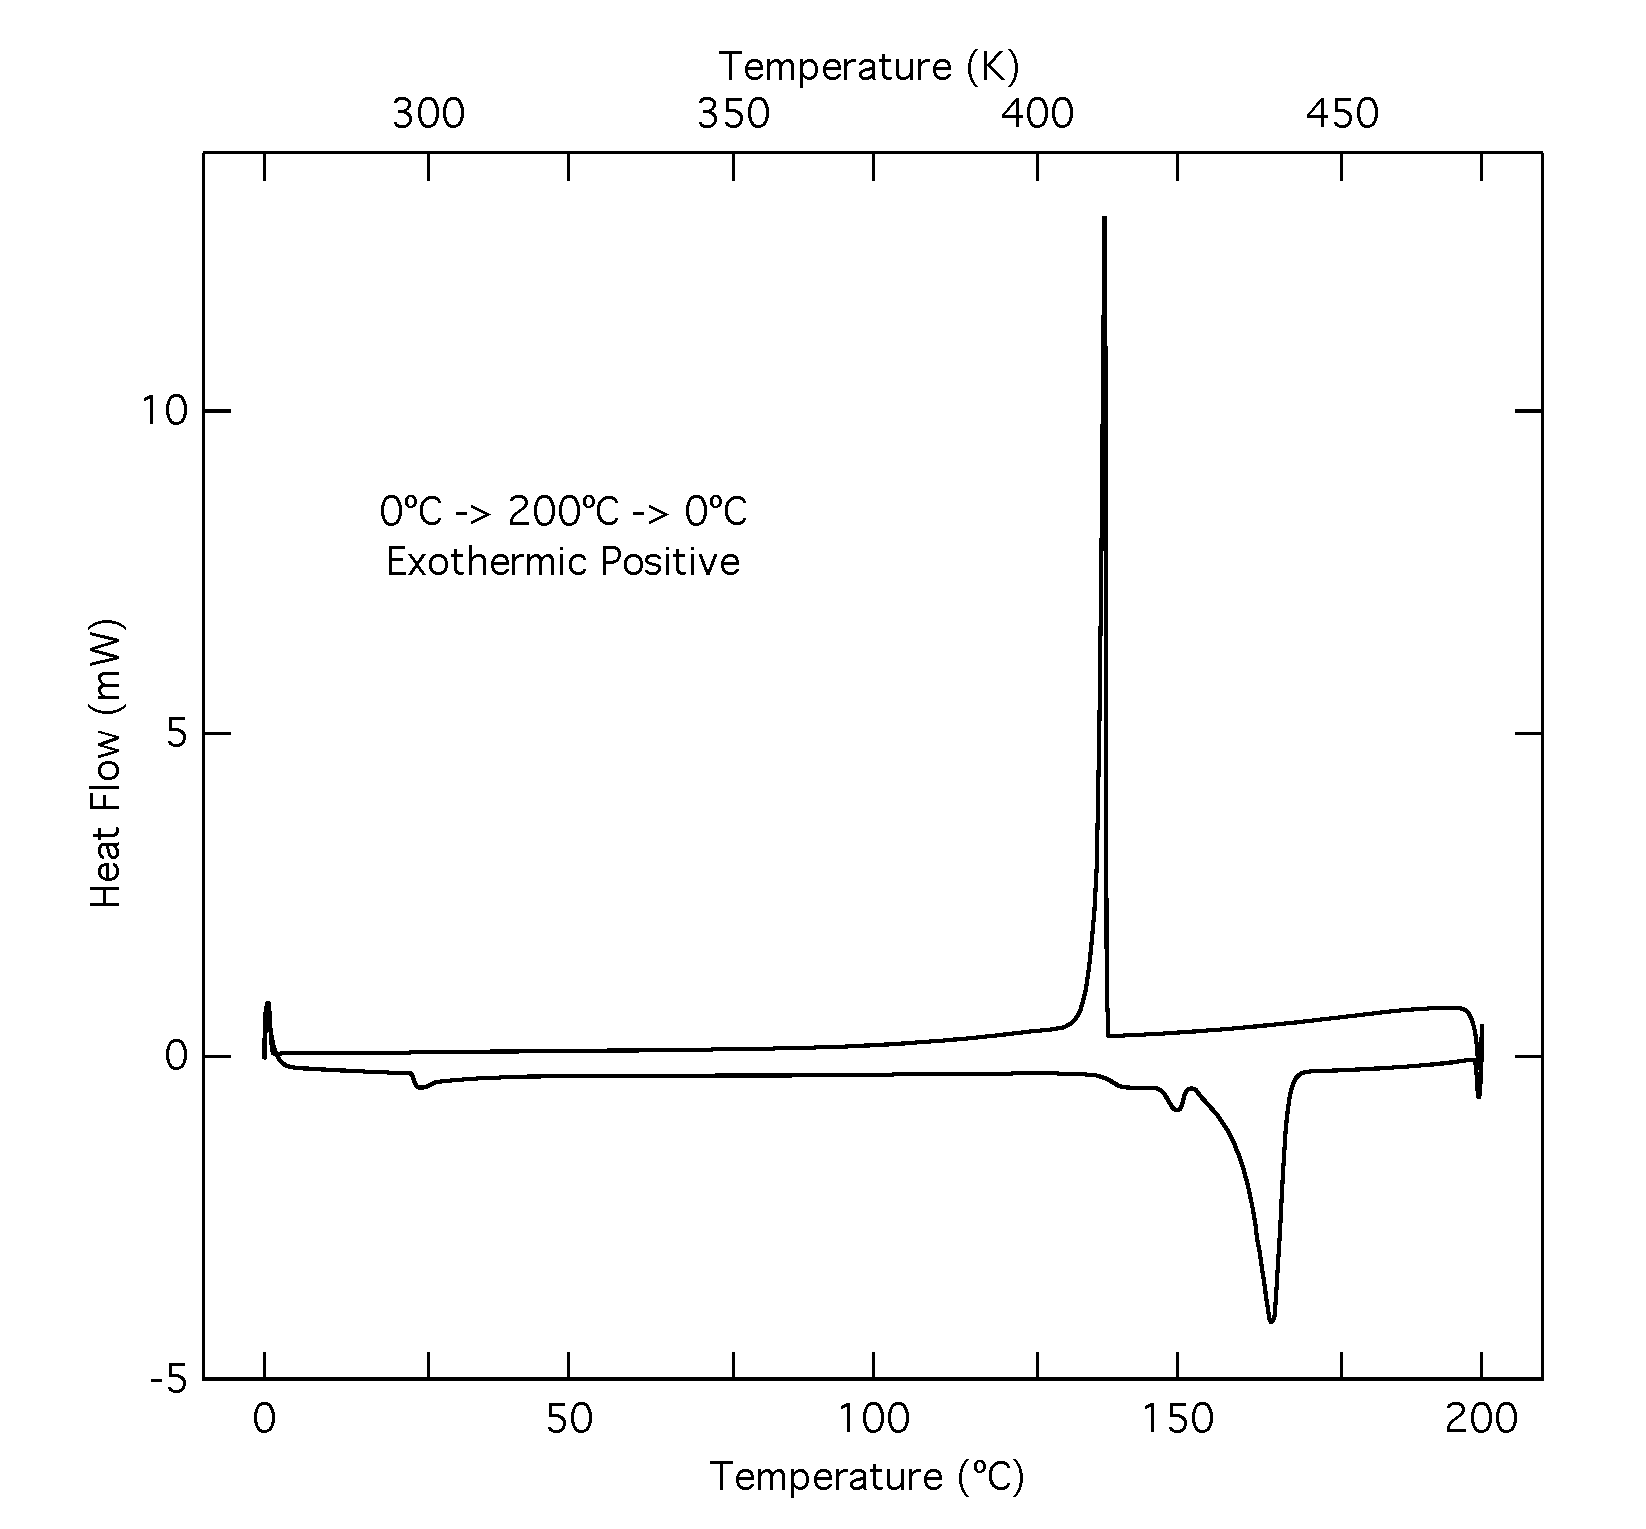
\includegraphics[width=0.66\textwidth]{./Figures/Data/Thermal-Analysis/DSC/HFAc}
	\caption[DSC Results of \HFAc{}]%
		{Plot of the DSC scan of \HFAc{}. In this plot exothermic behavior, where the sample releases heat, is %
		considered positive. Thus, the first sweep of the scan (from 0\degC{} to 200\degC{}) is negative. %
		Sample mass: 4.7 mg.}
	\label{fig:DSC-HFAc}
\end{figure}

Similarly, when \TMHD{} is heated to moderate temperatures (up to 200\degC{}, see fig~\vref{fig:DSC-TMHD-200}), such as those used in the evaporation and transport stages of the ALD system, there are no irregularities in the data. There is also no net energy gain or loss during the test indicating that heating up to 200\degC{}, along with the associated melting and freezing of the compound, is not detrimental to its structure. 

If the test is again performed, but with a higher upper temperature bound, the data is drastically different (see fig.~\vref{fig:DSC-TMHD-300}). As the sample is heated up to 300\degC{}, there are a number of significant energy releases that occur. These processes initiate at 234\degC{}, and are due to the precursor undergoing pyrolysis reactions. As such, this sets the safe upper temperature range for the ``ALD window'' of \TMHD{} at 230\degC{}. ALD reactions require that the precursor arrive to the surface intact and only react with surface species. 

\begin{figure}[tbp]
	\centering
	\subfloat[][Low Temperature Test (30--200--30\degC{})]{\label{fig:DSC-TMHD-200}%
		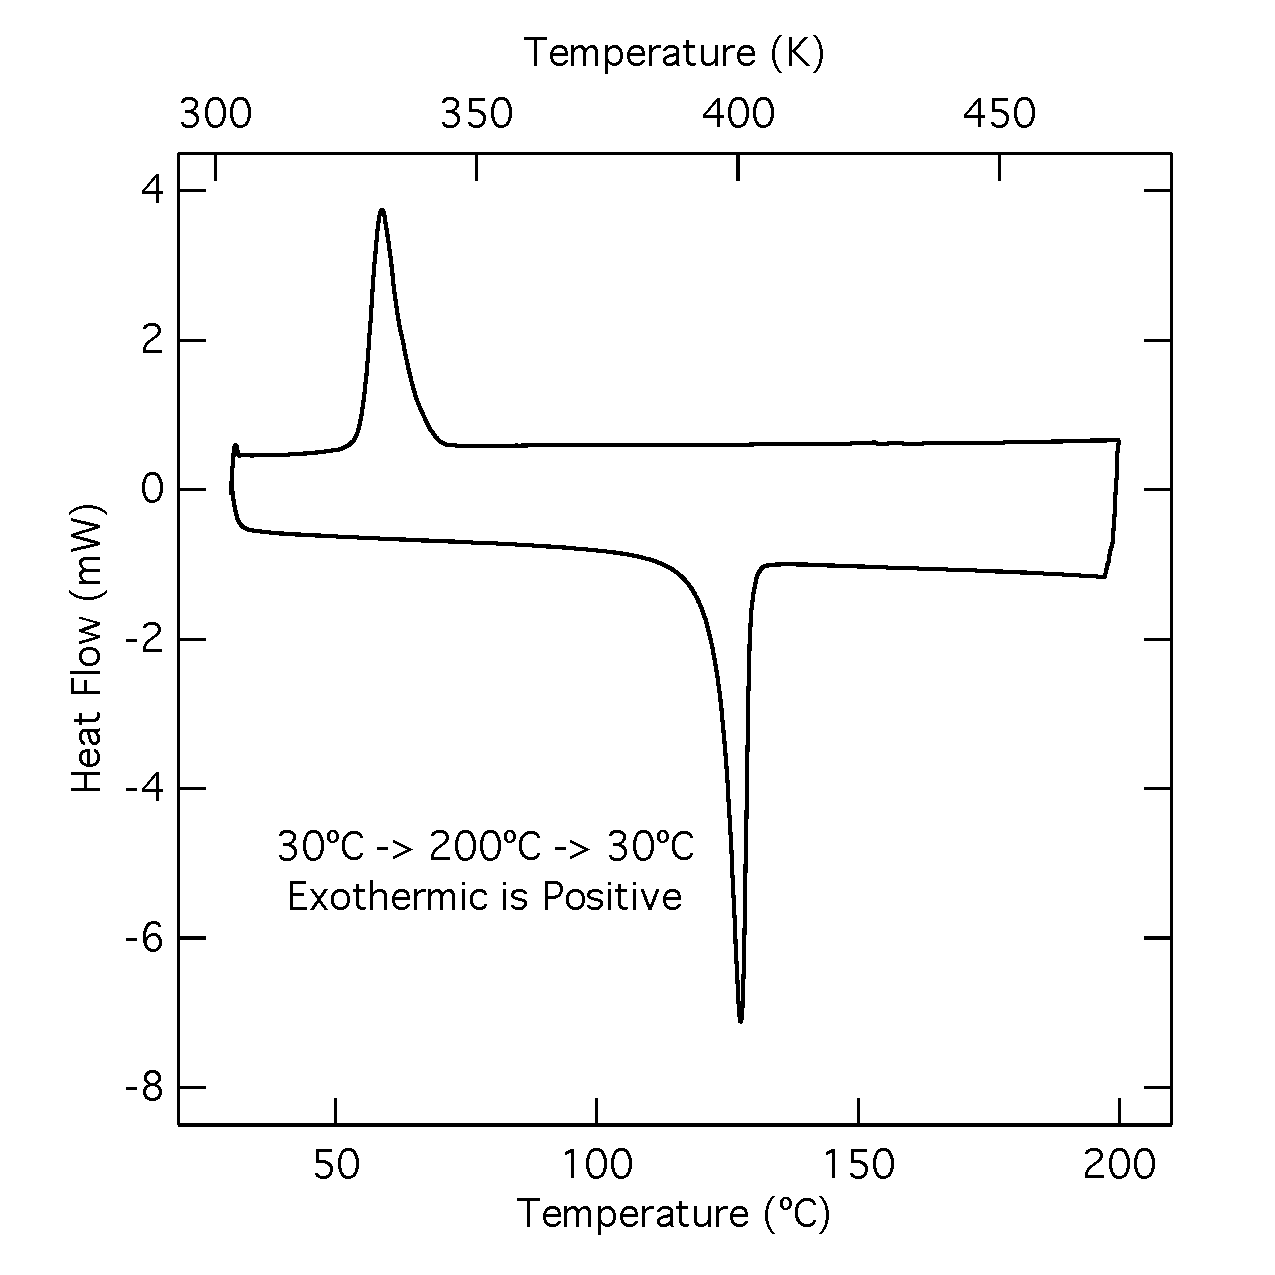
\includegraphics[width=0.66\textwidth]{./Figures/Data/Thermal-Analysis/DSC/TMHD-200}%
		}\\
	%\hspace{0.5cm}
	\subfloat[][High Temperature Test (30--300-30\degC{})]{\label{fig:DSC-TMHD-300}%
		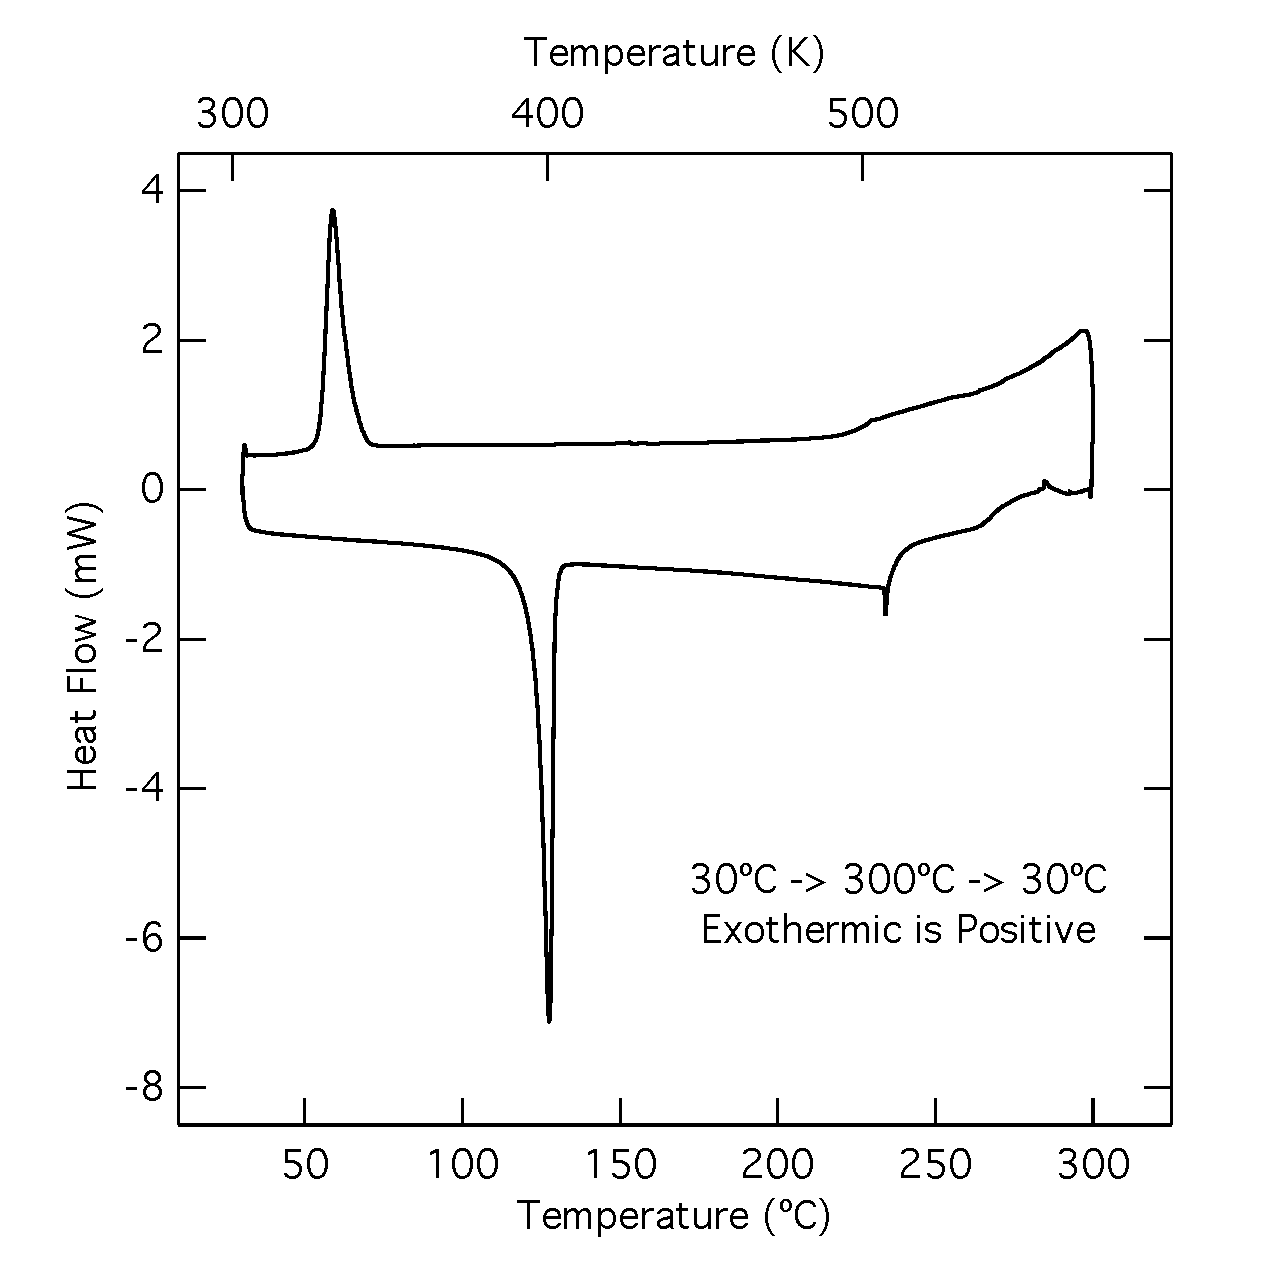
\includegraphics[width=0.66\textwidth]{./Figures/Data/Thermal-Analysis/DSC/TMHD-300}%
		}
	\caption[DSC Results of \TMHD{}]%
		{Results from the DSC scans of \TMHD{}. (a) Temperatures up to 200\degC{} show no change in the %
		material other than that of melting and freezing. (b) As temperatures increase, features start to appear %
		indicating chemical reconfiguration of the molecule.}
	\label{fig:DSC-TMHD}
\end{figure}
\clearpage
%%%%%%%%%%%%%%%%%%%%%%%%%%%%%%%%%%%%%%%%%%%%%%%%%%%%%%%%%%
%%%%%%%%%%%%%%%%%%%%%%%%%%%%%%%%%%%%%%%%%%%%%%%%%%%%%%%%%%
%%%%%%%%%%%%%%%%%%%%%%%%%%%%%%%%%%%%%%%%%%%%%%%%%%%%%%%%%%

\section{List of Samples}
\label{chap:Results-Samples}

Based on the results from the thermal analysis, a number of samples were deposited with various deposition parameters. Information on the deposition parameters for each of the samples used in this study can be found in the following table~\vref{tbl:LoSamples}. A small number of samples were attempted at 200\degC{}, but it was quickly determined that 225\degC{} provided better growth behavior without risking thermal cracking of the precursor. 

{\small
\vspace{2em}
\begin{longtable}{cccccccc}
	\caption[List of Samples]{A list of samples produced during the course of this project.%
	\label{tbl:LoSamples}}\\
	\toprule
	&&&&&\multicolumn{3}{c}{Annealing}\\ \cmidrule{6-8}
	Temp.		&Run \#	&Pb:Ti	 	&Cycles 	&Subs. 	&Type	&Temp. 		&Time\\ 
	(\degC{})		&		&Ratio		&		&Type	&		&(\degC{})	&(min)\\ \midrule%
	\endfirsthead
	\caption[]{A list of samples used during the course of this project.}\\
	\toprule
	&&&&&\multicolumn{3}{c}{Annealing}\\ \cmidrule{6-8}
	Temp.		&Run \#	&Pb:Ti	 	&Cycles 	&Subs. 	&Type	&Temp. 		&Time \\ 
	(\degC{})		&		&Ratio		&		&Type	&		&(\degC{})	&(min) \\ \midrule%
	\endhead
	200	&3		&1:1		&250	&Si		&None	&N/A		&N/A		\\
		&2		&1:2		&250	&Si		&None	&N/A		&N/A		\\
		&30		&3:1		&160	&Si		&None	&N/A		&N/A		\\
		&		&		&		&Pt-Si	&None	&N/A		&N/A		\\ \midrule
	225	&0		&1:1		&625	&Si		&Oven	&650	&120	\\
		&		&		&		&		&Oven	&900	&120	\\
		&		&		&		&		&RTA	&900	&10		\\
		&1		&1:1		&475	&Si		&None	&N/A		&N/A		\\
		&6		&1:2		&250	&Si		&None 	&N/A		&N/A		\\
		&13		&3:1		&250	&Si		&None 	&N/A		&N/A		\\
		&16		&3:1		&150	&Si		&RTA	&650	&1		\\
		&19		&3:1		&100	&Si		&None 	&N/A		&N/A		\\
		&		&		&		&Pt-Si	&None 	&N/A		&N/A		\\
		&20		&3:1		&200	&Si		&None 	&N/A		&N/A		\\
		&		&		&		&Pt-Si	&Oven	&650	&90		\\
		&		&		&		&STO	&Oven	&650	&90		\\
		&21		&3:1		&150	&Si		&None 	&N/A		&N/A		\\
		&		&		&		&Pt-Si	&Oven	&650	&90		\\
		&		&		&		&STO	&Oven	&650	&90		\\
		&22		&3:1		&150	&Si		&None 	&N/A		&N/A		\\
		&		&		&		&Pt-Si	&Oven	&650	&90		\\
		&23		&3:1		&200	&Si		&None 	&N/A		&N/A		\\
		&		&		&		&Pt-Si	&Oven	&650	&90		\\
		&28		&3:1		&120	&STO	&Oven	&650	&90		\\
	\bottomrule
\end{longtable}}

%%%%%%%%%%%%%%%%%%%%%%%%%%%%%%%%%%%%%%%%%%%%%%%%%%%%%%%%%%
%%%%%%%%%%%%%%%%%%%%%%%%%%%%%%%%%%%%%%%%%%%%%%%%%%%%%%%%%%
%%%%%%%%%%%%%%%%%%%%%%%%%%%%%%%%%%%%%%%%%%%%%%%%%%%%%%%%%%

\section{Ellipsometry}
\label{chap:Results-Ellipsometry}

Ellipsometry was a valuable tool during the course of this study. As discussed previously, it is capable of quickly, accurately, and non-destructively determine various properties of thin film layer stacks. Of primary importance is the ability of the tool to provide a rapid method of determining the thickness of a deposited layer. In ALD the growth rate is one of the primary markers of a well-tuned deposition process. An uncontrollably high growth rate is nearly as detrimental as having minimal growth. Varying deposition parameters and noting their effects on the growth rate of the process provided valuable insight into how best to tune the process. 

Given in table~\ref{tbl:LoThicknesses} is information on various samples and their as-deposited layer thicknesses, along with some relevant deposition parameters. One can also see from the plot of the sample thicknesses with respect to the number of deposition cycles (fig.~\vref{fig:Ellip-rates}) the consistency of a growth rate given a certain set of parameters. There is a small number of initial cycles required to initiate growth, referred to as ``incubation'' cycles, and then the film thickness follows a close linear dependence to the number of deposition cycles. This is indicative of a deposition that is operating within the ALD window and behaving well. From figure~\ref{fig:Ellip-rates} it was found that films deposited on silicon required approximately 10 cycles to initiate layer growth and subsequently grew at a rate of 3.78 \AA/cycle. For platinum coated silicon the incubation time was longer, an average of 36 cycles, but the films grew at a faster rate of 4.12 \AA/cycle. On STO crystals a 21 cycle incubation period was followed by a growth phase with a rate of 4.08 \AA/cycle. This varies greatly from values reported in table~\ref{tbl:LoThicknesses} as the growth rates reported here do not take into account the incubation time. The relatively constant number of initiation cycles has a seemingly greater effect on samples with low cycle counts; the incubation cycles take up a greater percentage of the total run and lower the growth rate accordingly. 

\begin{table}[tbp]
	\centering
	\small
	\caption[Sample Thicknesses and Growth Rates]%
		{Table of the film thicknesses and associated growth rates as measured by ellipsometry. Growth rates do %
		not take into account any incubation times for the films.}
	\label{tbl:LoThicknesses}
	\begin{tabular}{llllrr}
		\toprule
		Pb:Ti		&Sample	&Cycles		&Substrate	&Thickness	&Growth Rate	\\
		Ratio	&\#		&			&Type		&(nm)		&(\AA/cycle)	\\ \midrule
		1:1		&0		&625		&Si			&85.9		&1.37		\\
				&1		&475		&Si			&63.4		&1.33		\\
		3:1		&13		&250		&Si			&*32.9		&*1.31		\\
				&16		&150		&Si			&51.2		&3.41		\\
				&19		&100		&Si			&34.3		&3.43		\\
				&		&			&Pt-Si		&27.5		&2.75		\\
				&20		&200		&Si			&71.8		&3.59		\\
				&		&			&Pt-Si		&64.4		&3.22		\\
				&		&			&STO		&73.6		&3.68		\\
				&21		&150		&Si			&53.2		&3.54		\\
				&		&			&Pt-Si		&45.8		&3.05		\\
				&		&			&STO		&52.9		&3.53		\\
				&22		&150		&Si			&53.3		&3.55		\\
				&		&			&Pt-Si		&46.5		&3.10		\\
				&23		&200		&Si			&72.0		&3.60		\\
				&		&			&Pt-Si		&64.6		&3.23		\\
				&28		&120		&STO		&41.0		&3.42		\\	
		\bottomrule
	\end{tabular}
\end{table}

\begin{figure}[tbp]
	\centering
	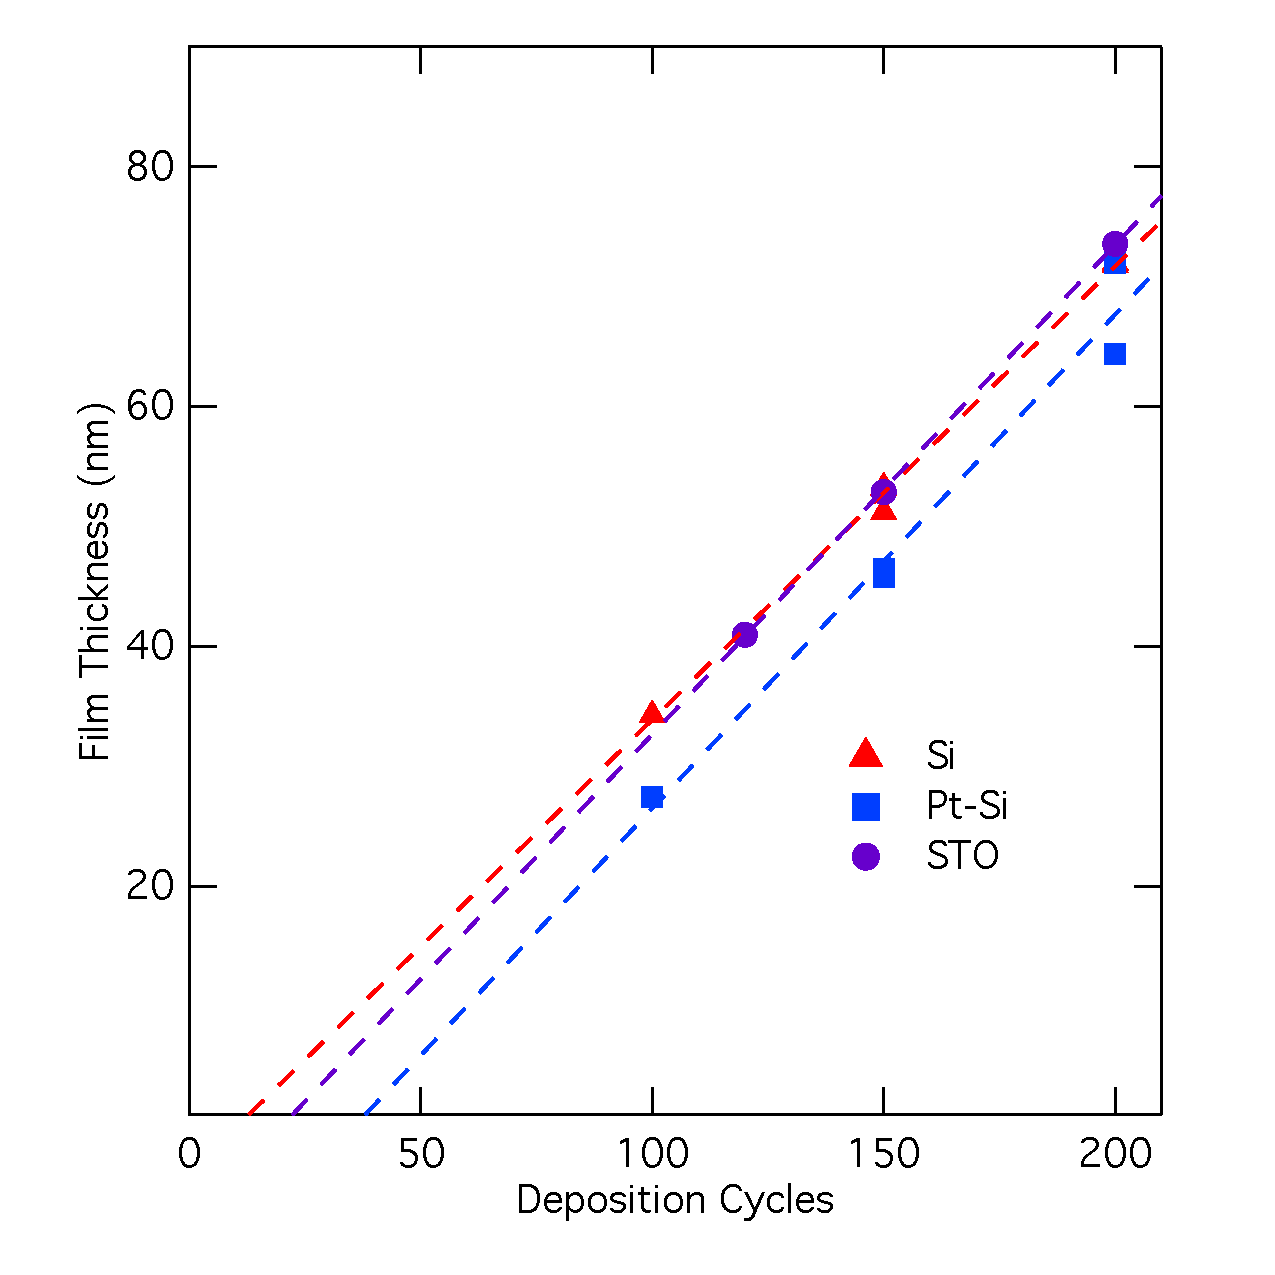
\includegraphics[width=0.6\textwidth]{./Figures/Data/Ellipsometry/Ellip-Rates}
	\caption[Film Thicknesses vs. Deposition Cycles]%
		{A plot of film thicknesses determined by ellipsometry. Growth rates and average incubation times are %
		extrapolated from this data. All films were deposited with a 3:1 Pb:Ti ratio and at 225\degC{}}
	\label{fig:Ellip-rates}
\end{figure}
	
An additional piece of information that can be extracted from ellipsometric analysis is an estimation of the band gap energy of the deposited layer. Because the final model used in the analysis method (see Section~\vref{chap:Methods-Ellip-Analysis}) is physically descriptive of the optical properties of the material, it is possible to extract such information from the model. By transforming the plot of the extinction coefficient, $k$, into that of the absorption coefficient, $\alpha$, it becomes possible to use the method developed by Tauc, \emph{et.al.} to determine the band gap energy of the material.\cite{tauc_optical_1968,ablees_optical_1972} However, such analysis does not take into account presence of multiple phases in the layer; when multi-phase layers are present the resulting band gap can only be used as a rough estimate. Tauc analysis also requires that the sample be properly crystallized, and thus must have undergone an annealing treatment before the analysis method becomes valid. As samples produced here had low phase purity, which will be discussed in subsequent sections, this analysis was of little use as a film benchmark. Some results from these analyses can be found in Appendix~\vref{sup:Ellipsometry}.

%%%%%%%%%%%%%%%%%%%%%%%%%%%%%%%%%%%%%%%%%%%%%%%%%%%%%%%%%%
%%%%%%%%%%%%%%%%%%%%%%%%%%%%%%%%%%%%%%%%%%%%%%%%%%%%%%%%%%
%%%%%%%%%%%%%%%%%%%%%%%%%%%%%%%%%%%%%%%%%%%%%%%%%%%%%%%%%%

\section{Composition}
\label{chap:Results-Composition}

Controlling the composition of the film was another primary task during the course of this project. Controlling the stoichiometry of the deposited films was of critical importance in obtaining films that presented the perovskite phase. If the balance of the two cations (\PbIon{} and \TiIon{}) was allowed to stray away from unity, other phases would be preferred or a mixture of phases would precipitate during a crystallizing heat treatment.  

As discussed previously, X-ray fluorescence was the method used for performing the composition analysis of the film structures. Through testing it was found that a deposition ratio of 3:1 in favor of the lead half-reaction provided the best film composition; there were a pair of samples deposited at an even 1:1 ratio that also provided near unity compositions (sample \#0 and \#1). A list of samples and their compositions, measured via XRF, can be found below (see table~\vref{tbl:XRF-compositions}). 

As mentioned in Section~\ref{sec:Methods-XRF}, samples deposited on STO were unable to have their compositions accurately measured using this technique. This was due to the confounding influence of the titanium content in the STO substrate, and there were no surface sensitive characterization methods available. 


\begin{table}[tbp]
	\centering
	\caption[XRF Calculated Compositions]{Calculated compositions of selected samples, determined via XRF. \\Composition percentages are all $\pm$1\%.}\label{tbl:XRF-compositions}
	\begin{tabular}{l l r r r}
	\toprule
	&&\multicolumn{3}{c}{Composition (\%)}\\
	\cmidrule{3-5}
	Run \#&Substrate&Lead&Titanium&Ti:Pb Ratio\\
	\midrule
% 	Run	Sub-Type		Pb%		Ti%		Ti:Pb ratio
	0	&\ce{SiO2}	&56.0	&44.0	&0.786\\
	1	&\ce{SiO2}	&55.0	&45.0	&0.809\\
	13	&\ce{SiO2}	&54.0	&46.0	&0.853\\
	16	&\ce{SiO2}	&49.4	&50.6	&1.022\\
	19	&\ce{SiO2}	&65.9	&34.1	&0.518\\
		&Pt-Si		&42.9	&57.1	&1.333\\
	20	&\ce{SiO2}	&56.6	&43.4	&0.769\\
		&Pt-Si		&51.5	&48.5	&0.944\\
	21	&\ce{SiO2}	&69.6	&30.4	&0.437\\
		&Pt-Si		&56.1	&43.9	&0.783\\
	22	&\ce{SiO2}	&67.7	&32.3	&0.478\\
		&Pt-Si		&56.1	&43.9	&0.784\\
	23	&\ce{SiO2}	&66.9	&33.1	&0.495\\
		&Pt-Si		&49.1	&50.9	&1.038\\
	24	&\ce{SiO2}	&69.0	&31.0	&0.450\\
		&Pt-Si		&62.2	&37.8	&0.609\\
	\bottomrule
	\end{tabular}
\end{table}
\clearpage
%%%%%%%%%%%%%%%%%%%%%%%%%%%%%%%%%%%%%%%%%%%%%%%%%%%%%%%%%%
%%%%%%%%%%%%%%%%%%%%%%%%%%%%%%%%%%%%%%%%%%%%%%%%%%%%%%%%%%
%%%%%%%%%%%%%%%%%%%%%%%%%%%%%%%%%%%%%%%%%%%%%%%%%%%%%%%%%%


\section{X-Ray Diffraction}
\label{chap:Results-XRD}


XRD was performed on a number of samples that had indicated composition ratios near unity. After an annealing treatment, generally performed in a regular ambient environment furnace but occasionally through use of the RTA, the XRD data was taken. However, samples processed using the RTA tended to obtain a unique and very rough surface texture, as opposed to the smooth mirror appearance of samples processed in the standard furnace. This observation lead to the adoption of the standard furnace as the main method of heat treatment. 

Analysis of XRD spectra made on the samples indicated a significant variety of phases present in the crystallized films. For example, figure~\vref{fig:XRD-0-Si-Full} gives the result from the sample \#0 deposited on a platinized silicon substrate. There are three major phases present: \ce{PbO2}, \ce{PbO}, and \PTO{}. The reflections from \PTO{} and lead(IV) oxide are much weaker than those from the lead(II) oxide. 

\begin{figure}[tbp]
	\centering
	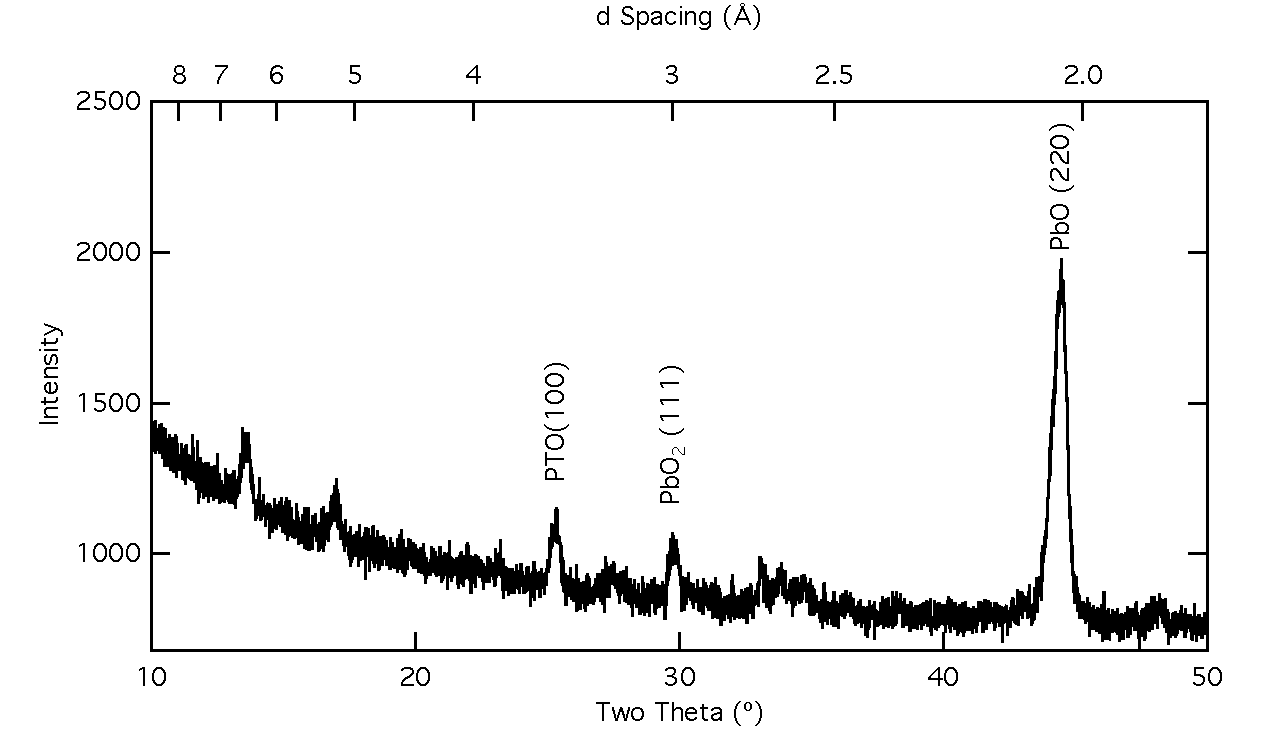
\includegraphics[width=0.95\textwidth]{./Figures/Data/XRD/Run-0-si/10-50}
	\caption[XRD Scan of \#0 on Si]%
		{This data shows the result of diffractometry on sample \#0 Pt-Si. From this, the %
		PTO(100) reflection can be identified, as well as some other lead oxide phases.}
	\label{fig:XRD-0-Si-Full}
\end{figure}

However, other samples produced more interesting films. For example, sample \#23 on Pt-Si (see figure~\vref{fig:XRD-20-Pt-Full}), has strong reflections from the \PTO{} (110) and (101) planes. There was a significant number of impurity phases present, often in significant amounts, such as the pyrochlore phases \ce{Pb2Ti2O6} and \ce{PbTi3O7}, which indicates issues during the crystallization phase of the sample processing. However, the presence of the desired perovskite phase marked an important point in the course of this study, as it showed that the process is capable of accomplishing the goal of \PTO{} via ALD methodology. 

\begin{figure}[tbp]
	\centering
	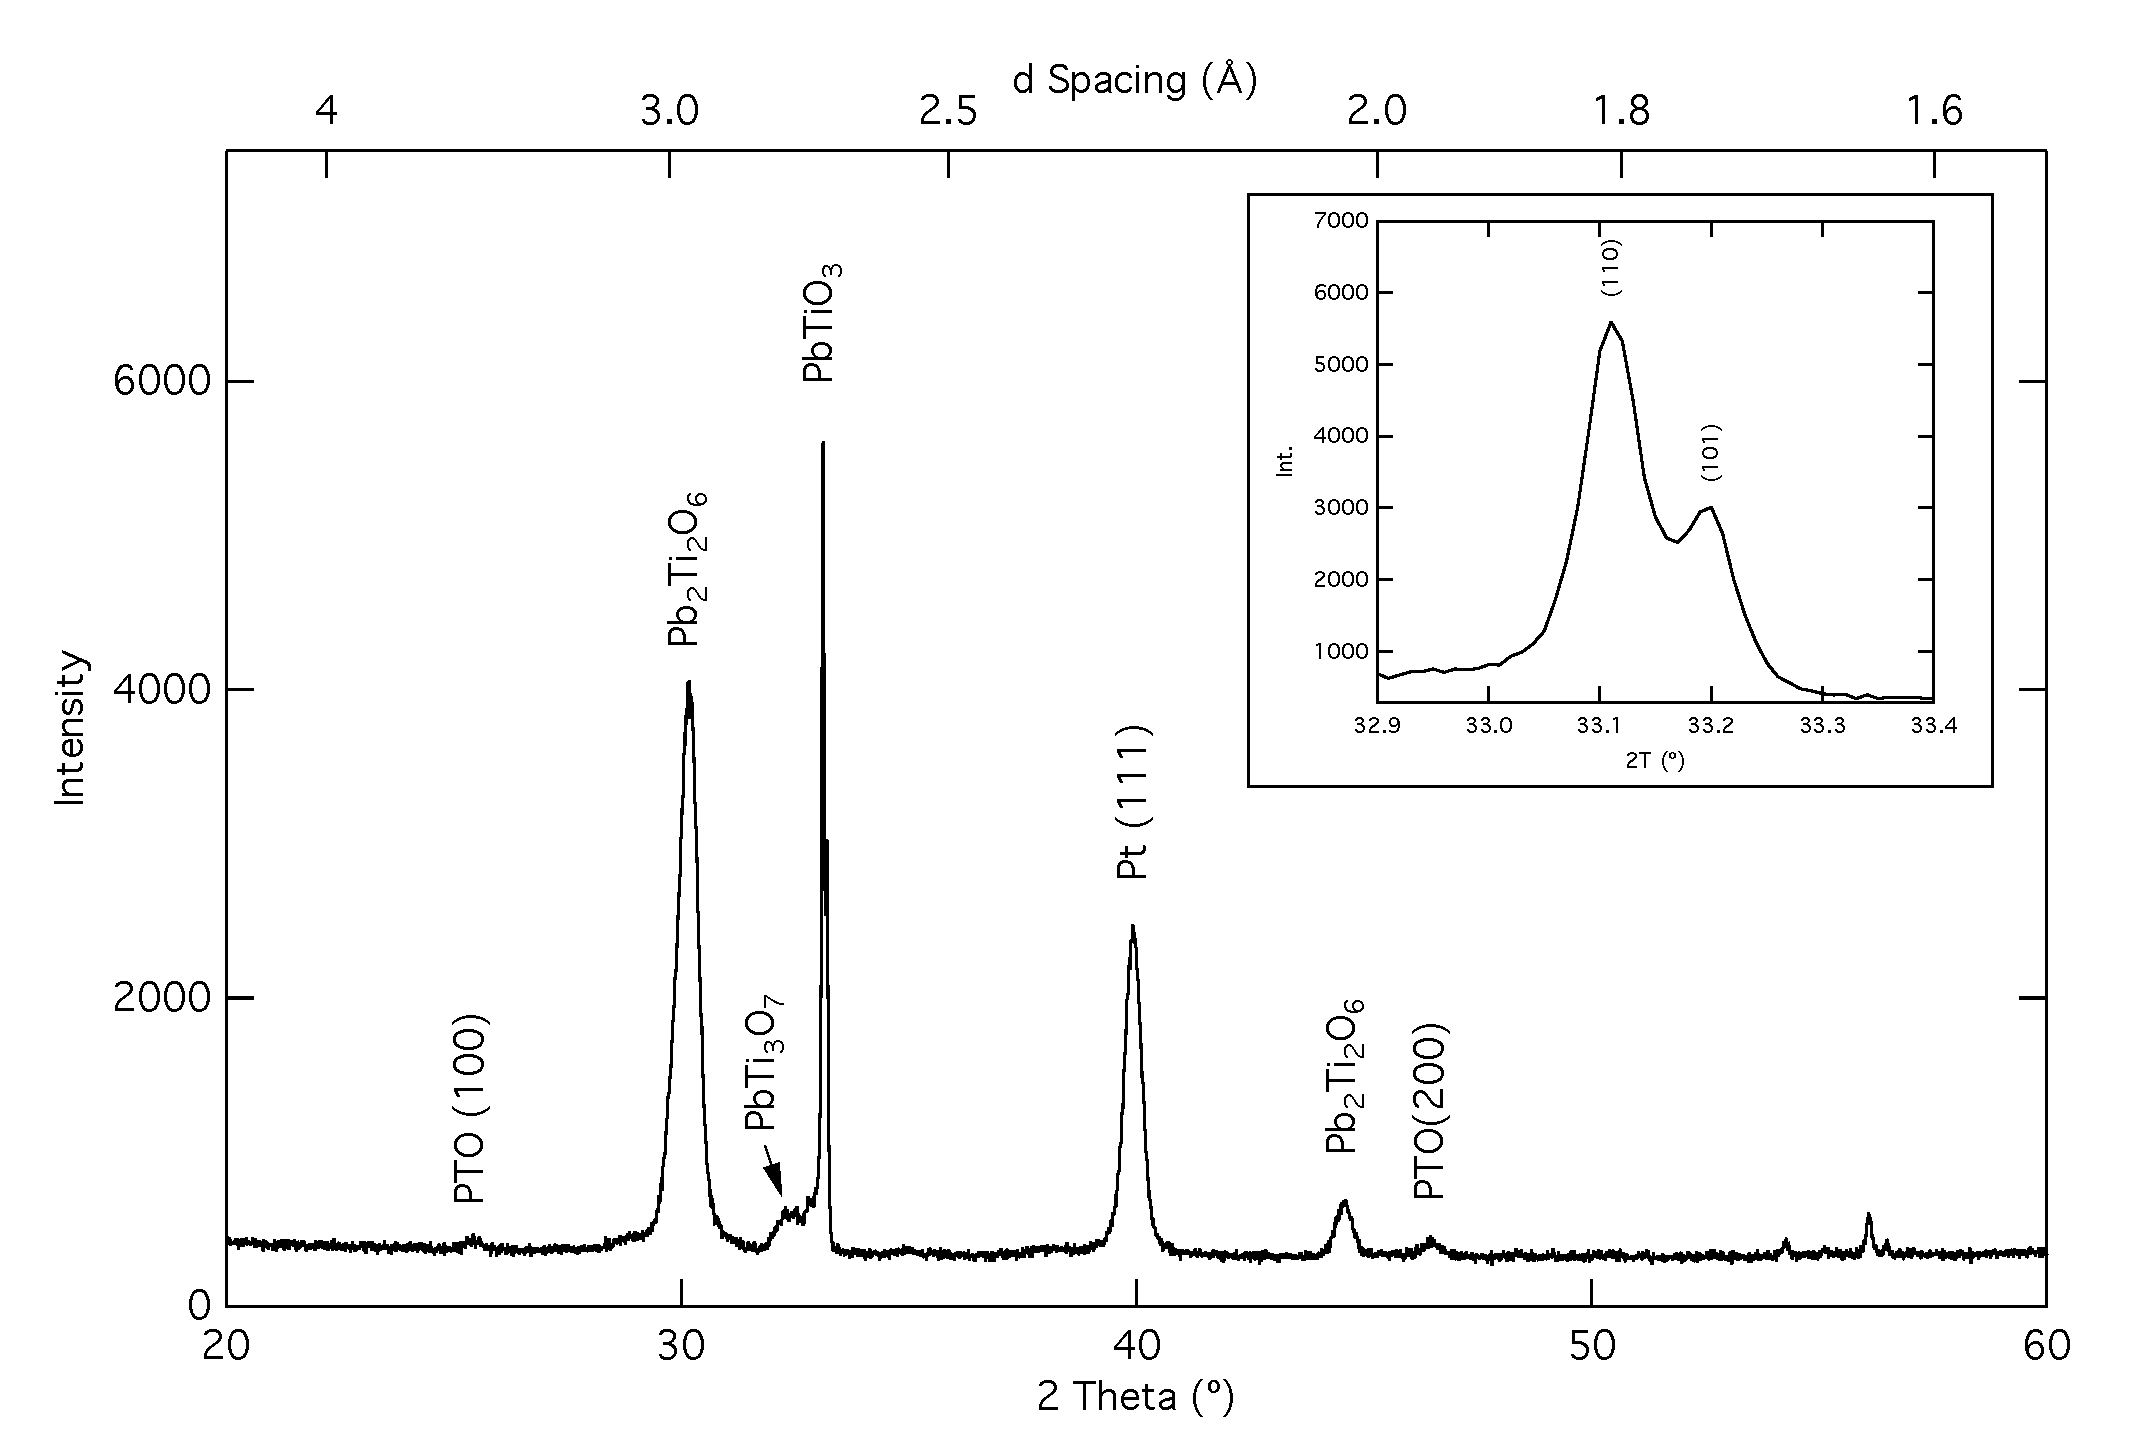
\includegraphics[width=0.95\textwidth]{./Figures/Data/XRD/Run-23-Pt/20-60}
	\caption[XRD Scan of \#23 on Pt]%
		{This data shows the result of diffractometry on sample \#23 Pt-Si. In this sample  a variety of phases %
		are present. The inset shows the splitting of the \PTO{} peak, due to the tetragonal nature of its %
		unit cell.}
	\label{fig:XRD-23-Pt-Full}
\end{figure}

Additional samples provided similar results. For example, \#20 on Pt-Si (fig.~\vref{fig:XRD-20-Pt-Full}), has similar impurities but again exhibits an abundance of the \PTO{} phase. This sample has a slightly higher concentration of \ce{PbTi3O7}, and a slightly weaker reflection from the dominant PTO planes. 

\begin{figure}[tbp]
	\centering
	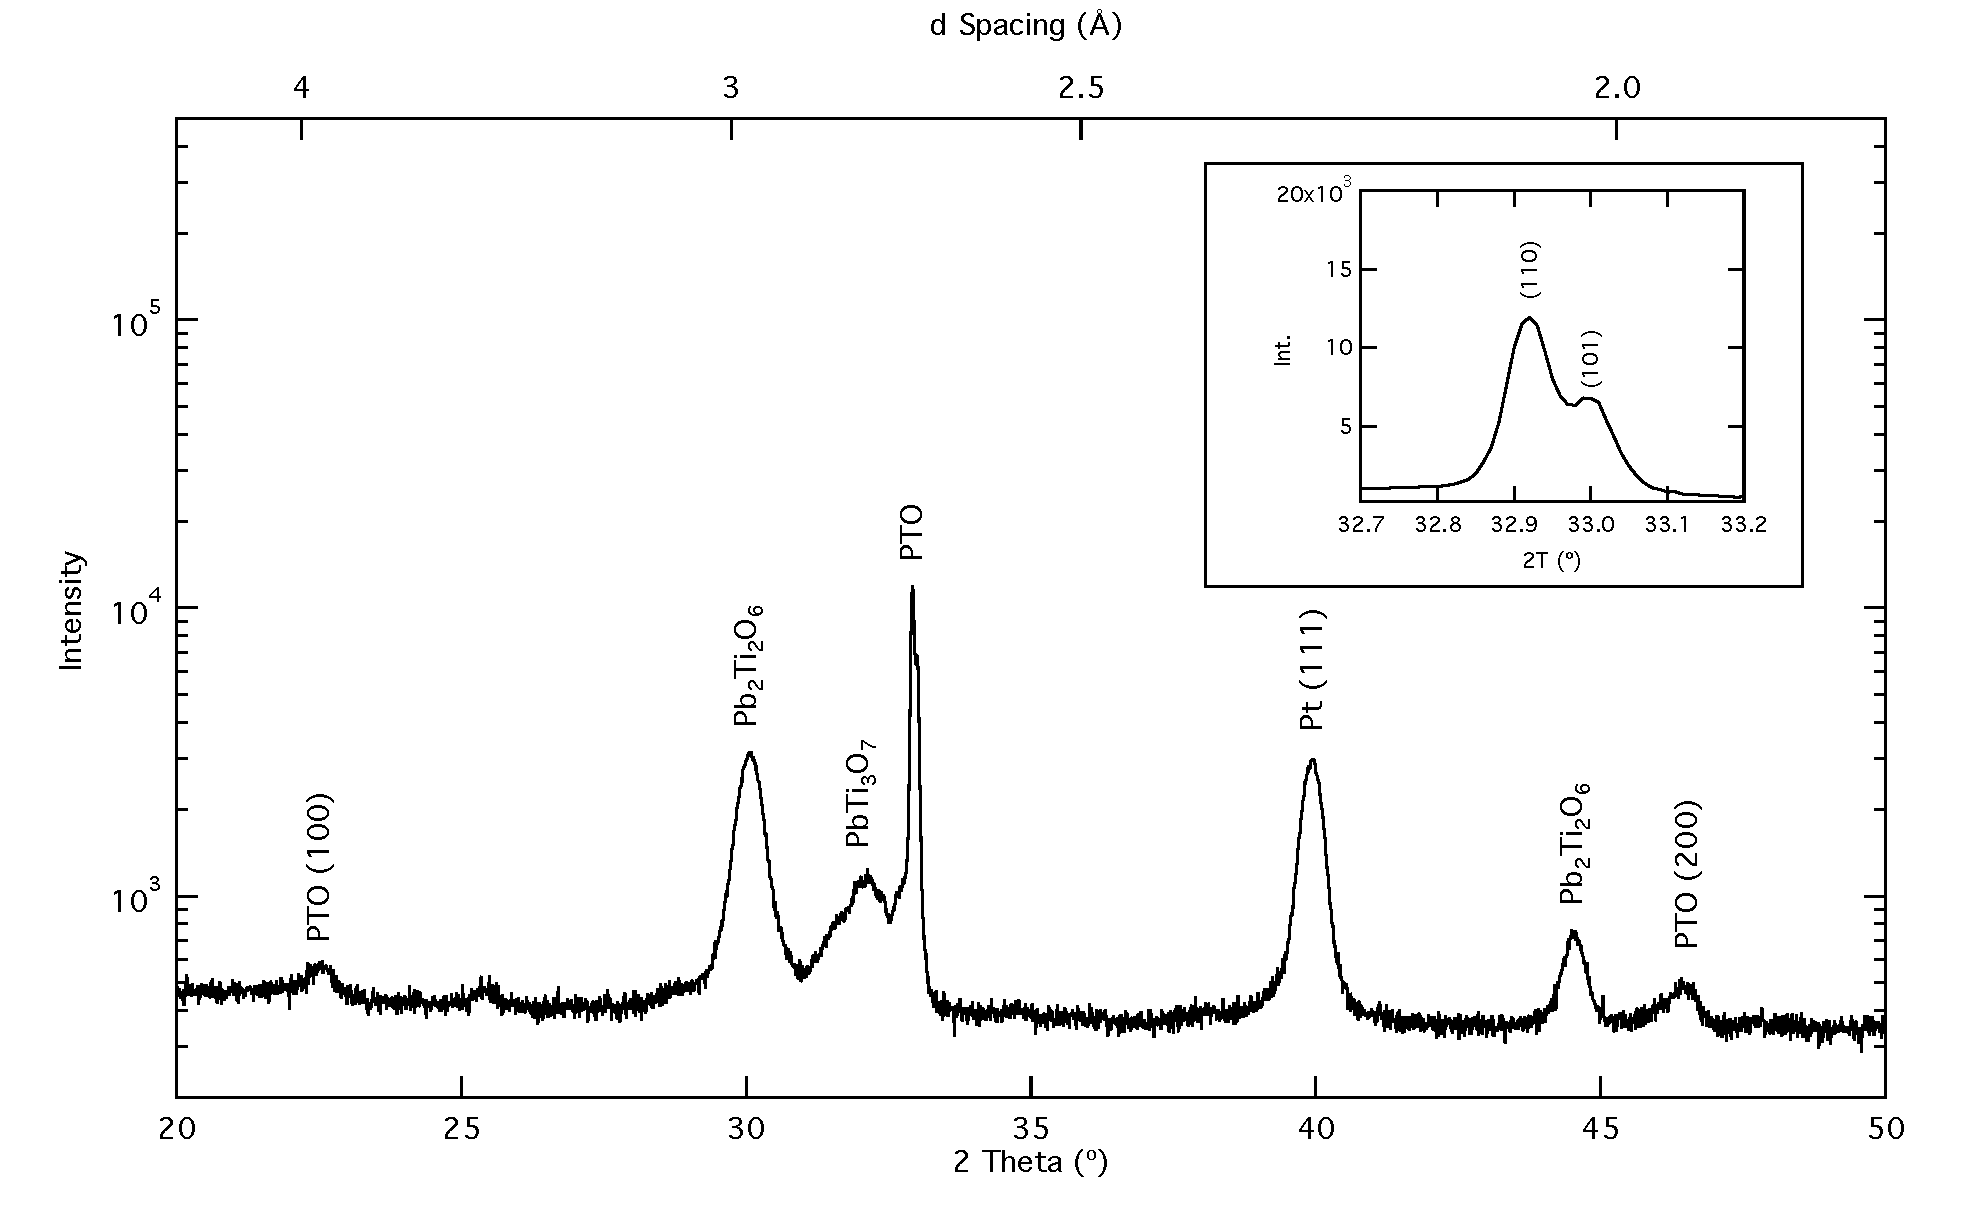
\includegraphics[width=0.95\textwidth]{./Figures/Data/XRD/Run-20-Pt/20-50}
	\caption[XRD Scan of \#20 on Pt-SI]%
		{This data shows the result of diffractometry on sample \#20 Pt-Si. There are some impurity phases %
		present, however the strongest signals are due to the \\\PTO{} (101) and (110) reflections (see inset).}
	\label{fig:XRD-20-Pt-Full}
\end{figure}

Finally, investigation of a sample deposited on strontium titanate crystal (see figure~\vref{fig:XRD-28-STO-Full}) showed a strong preference of the PTO phase to orient with the orientation of the substrate. In this sample was also seen presence of titania phases (rutile, $\alpha$-\ce{TiO2}) as composed to samples deposited on Si and Pt-Si substrates. However, since the precise composition of films on STO is unknown the reason for finding \ce{TiO2} is unclear, likely due to an excess of titanium in the deposited film. 

\begin{figure}[tbp]
	\centering
	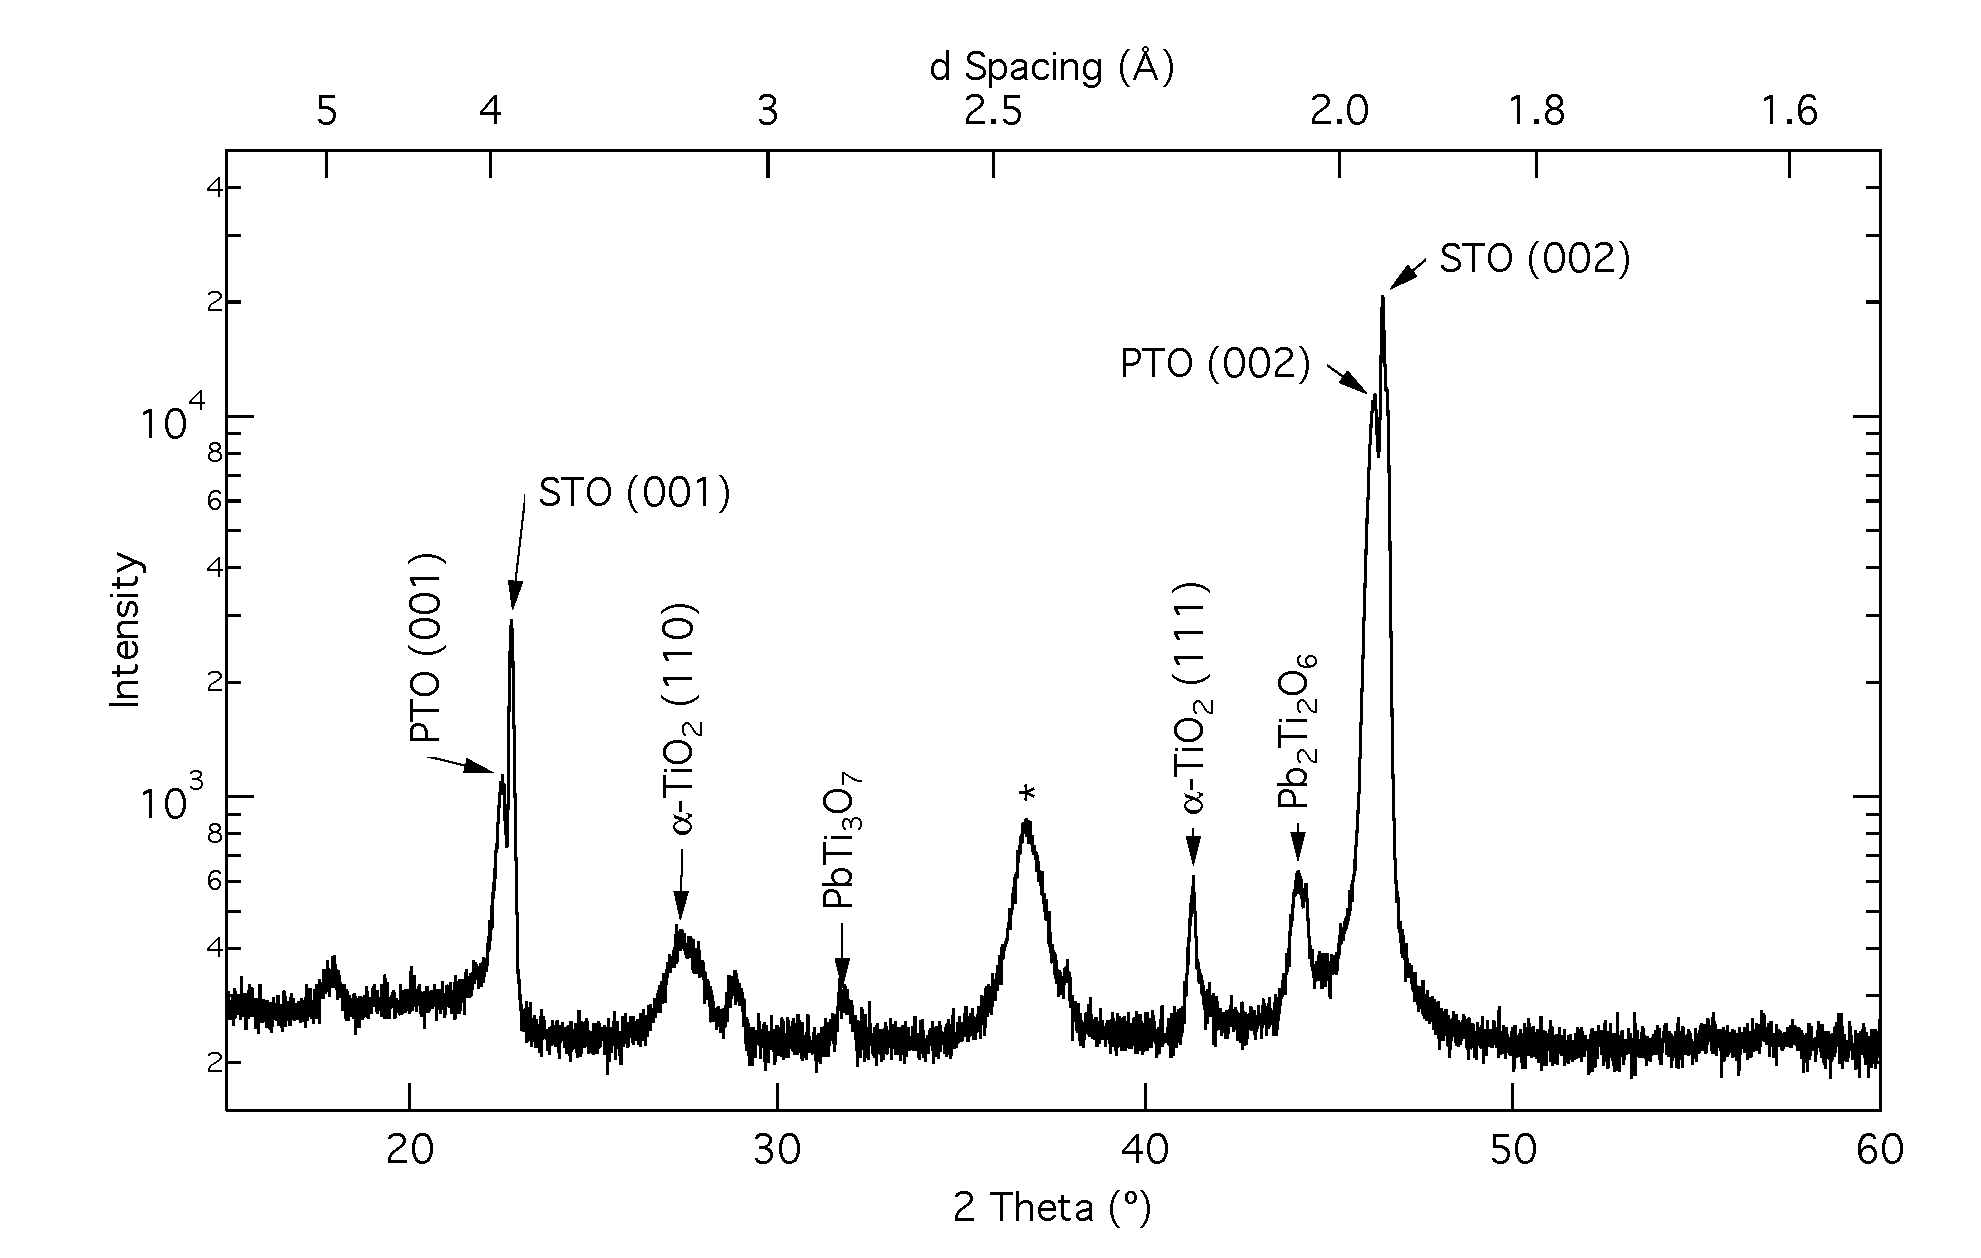
\includegraphics[width=0.95\textwidth]{./Figures/Data/XRD/Run-28-STO/15-60}
	\caption[XRD Scan of \#28 on STO]%
		{This data shows the result of diffractometry on sample \#28 STO. Impurity phases were present %
		(particularly $\alpha$-\ce{TiO2} and pyrochlore). It was also notable that the PTO phase preferentially %
		oriented itself with the STO (001) substrate.}
	\label{fig:XRD-28-STO-Full}
\end{figure}


















\chapter{Conclusions}
\label{ch:Conc}
\thispagestyle{empty}


The final result of this study was to show that it is certainly possible to grow perovskites using an ALD process, but the exact processes are sensitive and require much attention and further analysis.  

At the completion of this project, it can be said that the following goals have been met. A method for analyzing and predicting the behavior and operating windows of potential ALD precursors using standard thermal analysis techniques (TGA and DSC) has been proposed and shows good promise for applicability towards other material systems and precursor.\cite{Broido_TGA_1969,skoog_DSC_1998,wunderlich_thermal_1990}

A reliable method of analyzing film thicknesses and growth rates has been developed utilizing ellipsometry, which allows for rapid and non-destructive testing (and possibly incorporation as an \emph{in situ} testing mechanism to monitor film growth during deposition). In addition, the method described is capable of extracting additional information about film properties (e.g. band gap energies and other electronic characteristics) that could be applied given a higher degree of phase purity in the final crystallized film.\cite{Bruzzese_2010,schubert_infrared_2005,tompkins_spectroscopic_1999}

Use of XRF, in place of the more common EDS, allowed for the quantitative analysis of film composition even at ultra thin thicknesses. This rapid and non-destructive tool was of significant utility to this project. However, the ability to perform surface sensitive measurements would have made analysis of films grown on strontium titanate crystals more complete.\cite{Vincze_XRF_2005}

It was found that phase identification was possible using XRD with the thin films produced in this study. However, utilization of grazing incidence XRD --- a technique used to improve surface sensitivity of XRD --- would likely improve upon the results seen here, and would likely prove necessary if films of lower thicknesses were to be analyzed. \cite{giacovazzo_XRD_1992}

It proved to be non-trivial to produce films which, upon annealing, crystallized into phase-pure perovskite \PTO{}. Instead, the films often degrade into a mixture of PTO, pyrochlore forms (\ce{PbTi3O7} and \ce{Pb2Ti2O6}), various lead oxides (\ce{PbO_{x}}), and rutile tiania. At this time it is unclear exactly what causes this behavior. Additional research into the thermodynamics and crystallization behavior of these films would be of great value. 

%%%%%%%%%%%%%%%%%%%%%%%%%%%%%%%%%%%%%%%%%%%%%%%%%%%%%%%%%%
%%%%%%%%%%%%%%%%%%%%%%%%%%%%%%%%%%%%%%%%%%%%%%%%%%%%%%%%%%
%%%%%%%%%%%%%%%%%%%%%%%%%%%%%%%%%%%%%%%%%%%%%%%%%%%%%%%%%%

\section{Future Work}
\label{sec:Conc-Future}

While the work presented herein is noteworthy, and lays a framework for further investigation and refinement of ALD deposited perovskite oxides including the topic of discussion of this thesis, there is much left to be investigated in this line of research. Next steps would serve to further refine the process to improve the reliability of deposition, improving the phase purity and improve the degree of epitaxy of the grown film, or better conserve and deliver precursor (issues that plagued this project throughout its course). Being able to consistently produce films of constant quality would make this work applicable to a myriad of material systems. 

Additionally, there is one aspect of film characterization that had not been investigated thoroughly during the course of this project: the ferroelectric character of the films. Verification of ferroelectric behavior, even initially in isolated grains, would greatly improve the value of the method. Initial tests would likely require the use of microscopy techniques, e.g. piezoelectric force microscopy (PFM), to measure response of isolated grains of ferroelectric material; more standard ferroelectric measurements could likely be utilized with improved film quality and phase purity. 

Following this path of discussion quickly leads to the question of doping the films in order to improve properties. The obvious example here would be the development of an ALD process for \ce{PbZr_{0.52}Ti_{0.48}O3}. Lead titanate as a material is rather uncommonly used in applications, however as a simplified example of this family it was a prime candidate for the primary research. This project thus serves as a gateway to exploring the more valuable and technically relevant materials via ALD. 

Finally, it would be useful to extend this method to completely new material families. (Ba,Sr)Ti\ce{O3} is another commonly used ferroelectric material. Use of this material is gaining interest not only due to its intrinsic properties, but also due to its lack of lead content which makes it a far more environmentally conscious choice. \ce{BiFeO3} and corresponding doped materials, are another interesting perovskite. This set of materials presents multiferroic --- a combination of (anti)ferromagnetism and ferroelectricity --- behavior, making it a prime target for such novel technologies as spintronics. 








%%% END OF CONTENT %%%

\cleardoublepage % Start new odd page


% ---- Bibliography ----
\fancyhead[RE]{\nouppercase{\bfseries\leftmark}}
\fancyhead[LO]{\nouppercase{\bfseries\rightmark}}
\fancyhead[RO,LE]{\bfseries\thepage}
\fancyfoot{}
\addcontentsline{toc}{chapter}{Bibliography} % Adds Bibliography chapter entry to ToC. 
\bibliographystyle{unsrt} % This will not sort the bibliography in anyway, but instead will sort by order of appearance in the document. Other styles available.

% Creates the bibliography from the file 'bib_thesis.bib'. Can reference multiple .bib files, just separate with commas
\begin{spacing}{1}
\bibliography{./bibliography/bib_thesis} 
\end{spacing}
\clearpage
%\nocite{*}  	% This will add any remaining entries in the BibTeX file to the bibliography, without citing it in the document. 


\appendix

\pagestyle{fancy} 
\fancyfoot{}                                               
\renewcommand{\chaptermark}[1]{\markboth{\appendixname\ \thechapter.\ #1}{}} 
\renewcommand{\sectionmark}[1]{\markright{\thesection.\ #1}}         
\fancyhead[LE,RO]{\bfseries\thepage}    
                                        
\fancyhead[RE]{\bfseries\leftmark}    
\fancyhead[LO]{\bfseries\rightmark}     
\renewcommand{\headrulewidth}{0.3pt} 



\chapter{Supplemental Information}
\label{chap:appendix}
\thispagestyle{empty}

%%%%%%%%%%%%%%%%%%%%%%%%%%%%%%%%%%%%%%%%%%%%%%%%%%%%
%%%%%%%%%%%%%%%%%%%%%%%%%%%%%%%%%%%%%%%%%%%%%%%%%%%%
%%%%%%%%%%%%%%%%%%%%%%%%%%%%%%%%%%%%%%%%%%%%%%%%%%%%

\section{List of Chemicals}
\label{sup:LoChemicals}

\begin{table}[h]
	\centering
	\small
	\caption[List of Compounds]{List of chemical compounds used during the course of this study.}
	\label{tbl:LoCompounds}
	\begin{tabular}{llrrl}
		\toprule
		Chemical				&Chemical 			&CAS \#		&Molec.	&Source	\\ 
		Name				&Formula				&			&Weight	&		\\\midrule
		Lead(II) hexafluoro- 		&\ce{Pb(C5O2HF6)2}	&19648-88-5	&621.29	&Strem Chemicals,\\	
		acetylacetonate		&					&			&		&Inc.\\
		Bis(2,2,6,6-tetramethyl	&\ce{Pb(C11H19O2)2}	&21319-43-7	&573.50	&Strem Chemicals,\\
		-3,5-heptanedionato)	&					&			&		&Inc.\\
		Lead(II)\\
		Titanium(IV)			&\ce{Ti[OCH(CH3)2]4}	&546-68-9	&284.25	&Strem Chemicals,\\
		i-propoxide			&					&			&		&Inc.\\\midrule	
		Isopropyl Alcohol (IPA)	&\ce{(CH3)2CHOH}		&67-63-0		&60.10	&Alfa Aesar\\
		Acetone				&\ce{C3H6O}			&67-64-1		&58.08	&Alfa Aesar\\
		Buffered Hydrofluoric	&\ce{NH4F}-\ce{HF}		&7664-39-3	&N/A		&Alfa Aesar\\
		Acid (BHF)			&					&\& 12125-01-8\\
		Ozone				&\ce{O3}				&10028-15-6	&48.00	&\\
		\bottomrule
	\end{tabular}
\end{table}

\clearpage

%%%%%%%%%%%%%%%%%%%%%%%%%%%%%%%%%%%%%%%%%%%%%%%%%%%%
%%%%%%%%%%%%%%%%%%%%%%%%%%%%%%%%%%%%%%%%%%%%%%%%%%%%
%%%%%%%%%%%%%%%%%%%%%%%%%%%%%%%%%%%%%%%%%%%%%%%%%%%%

%\begin{landscape}
%\section{List of Samples}
%\label{sup:LoSamples}

%{
%\begin{longtable}{c c c c c c c c c}
%	\caption[List of Samples]{A list of samples used during the course of this project.%
%	\label{tbl:LoSamples}}\\
%	\toprule
%	&&&&&\multicolumn{3}{c}{Annealing}&\\ \cmidrule{6-8}
%	Temp.		&Run \#	&Pb:Ti	 	&Cycles 	&Subs. 	&Type	&Temp. 		&Time &XRD\\ 
%	(\degC{})		&		&Ratio		&		&Type	&		&(\degC{})	&(min) &\\ \midrule%
%	\endfirsthead
%	\caption[]{A list of samples used during the course of this project.}\\
%	\toprule
%	&&&&&\multicolumn{3}{c}{Annealing}&\\ \cmidrule{6-8}
%	Temp.		&Run \#	&Pb:Ti	 	&Cycles 	&Subs. 	&Type	&Temp. 		&Time &XRD\\ 
%	(\degC{})		&		&Ratio		&		&Type	&		&(\degC{})	&(min) &\\ \midrule%
%	\endhead
%	200	&3		&1:1		&250	&Si		&None	&N/A		&N/A		&No\\
%		&2		&1:2		&250	&Si		&None	&N/A		&N/A		&No\\
%		&30		&3:1		&160	&Si		&None	&N/A		&N/A		&No\\
%		&		&		&		&Pt-Si	&None	&N/A		&N/A		&No\\ \midrule
%	250	&0		&1:1		&625	&Si		&Oven	&650	&120	&Yes\\
%		&		&		&		&		&Oven	&900	&120	&Yes\\
%		&		&		&		&		&RTA	&900	&10		&No\\
%		&1		&1:1		&475	&Si		&None	&N/A		&N/A		&No\\
%		&6		&1:2		&250	&Si		&None 	&N/A		&N/A		&No\\
%		&13		&3:1		&250	&Si		&None 	&N/A		&N/A		&No\\
%		&16		&3:1		&150	&Si		&RTA	&650	&1		&No\\
%		&19		&3:1		&100	&Si		&None 	&N/A		&N/A		&No\\
%		&		&		&		&Pt-Si	&None 	&N/A		&N/A		&No\\
%		&20		&3:1		&200	&Si		&None 	&N/A		&N/A		&No\\
%		&		&		&		&Pt-Si	&Oven	&650	&90		&Yes\\
%		&21		&3:1		&150	&Si		&None 	&N/A		&N/A		&No\\
%		&		&		&		&Pt-Si	&Oven	&650	&90		&No\\ \\
%		&22		&3:1		&150	&Si		&None 	&N/A		&N/A		&No\\
%		&		&		&		&Pt-Si	&Oven	&650	&90		&Yes\\
%		&23		&3:1		&200	&Si		&None 	&N/A		&N/A		&No\\
%		&		&		&		&Pt-Si	&Oven	&650	&90		&Yes\\
%		&28		&3:1		&120	&STO	&Oven	&650	&90		&Yes\\
%	\bottomrule
%\end{longtable}}
%\clearpage
%%%%%%%%%%%%%%%%%%%%%%%%%%%%%%%%%%%%%%%%%%%%%%%%%%%%
%%%%%%%%%%%%%%%%%%%%%%%%%%%%%%%%%%%%%%%%%%%%%%%%%%%%
%%%%%%%%%%%%%%%%%%%%%%%%%%%%%%%%%%%%%%%%%%%%%%%%%%%%
%\begin{landscape}
\section{ALD Reactor Diagram}
\label{sup:ALD-design}

\begin{figure}[htb]
   \centering
   \subfloat[Photograph][Photograph]{%
   	\label{fig:S100-photo}%
	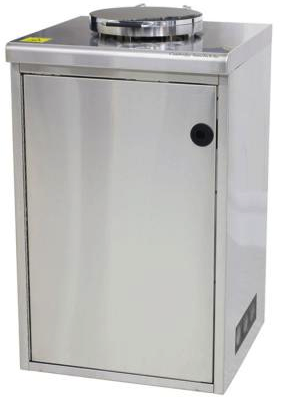
\includegraphics[height=8cm]{./Figures/Appendix/ALD-schematic/savannah-s100}%
	} 
	\hspace{1cm}
  \subfloat[Schematic Diagram][Schematic Diagram]{%
   	\label{fig:S100-schematic}%
	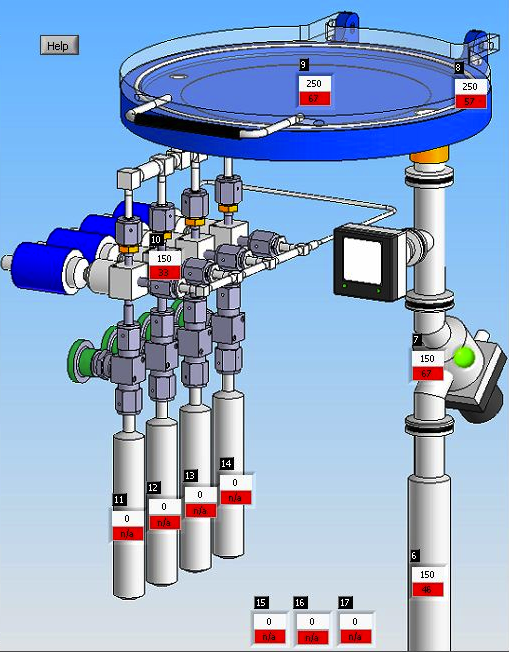
\includegraphics[height=8cm]{./Figures/Appendix/ALD-schematic/savannah-schematic}%
	} 	
   \caption[Cambridge NanoTech, inc. S100 ALD System]%
   		{Cambridge NanoTech, Inc. Savannah S100 ALD reactor. Precursors are stored in heated cylinders, flow up to the reaction zone, and byproducts are pumped out of the vacuum line on the right side. Each zone can be individually temperature controlled.\\\vspace{0.5em}%
		{\tiny Image Sources: (a) \url{http://www.cambridgenanotech.com/products/savannah.php} via %
		Cambridge NanoTech, Inc.\cite{CNT-web}\\%
		(b) Screenshot taken from Savannah ALD Control Software, via Cambridge NanoTech, Inc.\cite{CNT-web}}}
   \label{fig:S100}
\end{figure}

\clearpage
%
%\begin{figure}[htbp]
%	\begin{center}
%		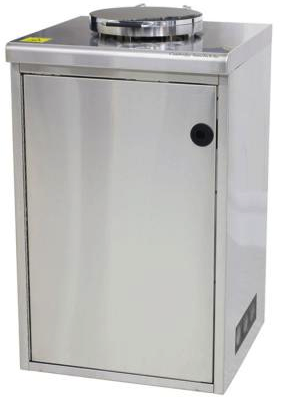
\includegraphics[width=0.5\textwidth]{./Figures/Appendix/ALD-schematic/savannah-s100}
%		\caption[Photograph of S100 ALD Reactor]{Photograph of the Cambridge NanoTech, inc. %
%				Savannah S100 ALD reactor}
%		\label{fig:S100-photo}
%	\end{center}
%\end{figure}
%
%\begin{figure}[htbp]
%	\begin{center}
%		\includegraphics[width=0.85\textwidth]{./Figures/Appendix/ALD-schematic/savannah-schematic}
%		\caption[Diagram of S100 ALD Reactor]{Diagram of the Cambridge NanoTech, inc. %
%				Savannah S100 ALD reactor. Precursors are stored in heated cylinders, flow up to the reaction zone, and byproducts are pumped out of the vacuum line on the right side. Each zone can be individually temperature controlled. }
%		\label{fig:S100-schematic}
%	\end{center}
%\end{figure}


%\end{landscape}
%%%%%%%%%%%%%%%%%%%%%%%%%%%%%%%%%%%%%%%%%%%%%%%%%%%%
%%%%%%%%%%%%%%%%%%%%%%%%%%%%%%%%%%%%%%%%%%%%%%%%%%%%
%%%%%%%%%%%%%%%%%%%%%%%%%%%%%%%%%%%%%%%%%%%%%%%%%%%%

%\section{Recipes for S100 ALD System}
%\label{sup:recipes}
%
%Should recipes be provided? They'd be rather specific to the instrumentation, and some of the recipes are provided by CNT (able to freely publish them?). This section would be trivial to construct, or remove entirely. 
%%
%%Provided in this section are recipes for the deposition of materials in the \ce{Pb_{x}Ti_{y}O_{z}} system. 
%%Some of these recipes (\ce{HfO2}, \ce{Pt}, and \ce{TiO2}) were provided courtesy of Cambridge NanoTech, inc.\cite{CNT-web} 
%%
%\clearpage
%%%%%%%%%%%%%%%%%%%%%%%%%%%%%%%%%%%%%%%%%%%%%%%%%%%%
%%%%%%%%%%%%%%%%%%%%%%%%%%%%%%%%%%%%%%%%%%%%%%%%%%%%
%%%%%%%%%%%%%%%%%%%%%%%%%%%%%%%%%%%%%%%%%%%%%%%%%%%%

%\section{Thermal Analysis Results}
%\label{sup:Thermal-Results}
%
%\subsection{Thermogravimetric Analysis}
%\label{sup:Thermal-Results-TGA}
%
%%\begin{figure}[htbp]
%%   \centering
%%   \subfloat[Mass vs. Temperature][Mass vs. Temperature]{%
%%   	\label{fig:TGA-HFAc-Weight}%
%%	\includegraphics[width=0.5\textwidth]{./Figures/Appendix/Thermal-Analysis/TGA/HFAc-Weight}%
%%	} \\
%%%	\hspace{1cm}
%%  \subfloat[Derivative of Mass vs. Temperature][Derivative of Mass vs. Temperature]{%
%%   	\label{fig:TGA-HFAc-DWeight}%
%%	\includegraphics[width=0.5\textwidth]{./Figures/Appendix/Thermal-Analysis/TGA/HFAc-DWeight}%
%%	} 	
%%   \caption[TGA Results for Pb(HFAc)$_{2}$ Precursor]%
%%   		{Plots of the results from TGA experiments on Pb(HFAc)$_{2}$. The plot shown in (a) gives the raw %
%%		data showing the current mass as a function of temperature. (b) gives the same data, transformed %
%%		to show the derivative of mass. Thus (b) shows the rate of mass loss at a given temperature. Initial %
%%		sample mass: 6.092 mg}
%%   \label{fig:TGA-HFAc}
%%\end{figure}
%%
%%\begin{figure}[htbp]
%%   \centering
%%   \subfloat[Mass vs. Temperature][Mass vs. Temperature]{%
%%   	\label{fig:TGA-TMHD-Weight}%
%%	\includegraphics[width=0.75\textwidth]{./Figures/Appendix/Thermal-Analysis/TGA/TMHD-Weight}%
%%	} \\
%%%	\hspace{1cm}
%%  \subfloat[Derivative of Mass vs. Temperature][Derivative of Mass vs. Temperature]{%
%%   	\label{fig:TGA-TMHD-DWeight}%
%%	\includegraphics[width=0.75\textwidth]{./Figures/Appendix/Thermal-Analysis/TGA/TMHD-DWeight}%
%%	} 	
%%   \caption[TGA Results for Pb(HFAc)$_{2}$ Precursor]%
%%   		{Plots of the results from TGA experiments on Pb(TMHD)$_{2}$. As in figure~\vref{fig:TGA-HFAc}, (a) %
%%		presents the actual mass as a function of temperature, while (b) gives the derivative of that function. %
%%		Initial sample mass: 3.719 mg}
%%   \label{fig:TGA-TMHD}
%%\end{figure}
%
%
%%\begin{figure}[htbp]
%%   \centering
%%   \subfloat[\HFAc][\HFAc]{%
%%   	\label{fig:TGA-HFAc-Hold}%
%%	\includegraphics[width=0.75\textwidth]{./Figures/Appendix/Thermal-Analysis/TGA/HFAc-Hold}%
%%	} \\
%%%	\hspace{1cm}
%%  \subfloat[\TMHD][\TMHD]{%
%%   	\label{fig:TGA-TMHD-Hold}%
%%	\includegraphics[width=0.75\textwidth]{./Figures/Appendix/Thermal-Analysis/TGA/TMHD-Hold}%
%%	} 	
%%   \caption[Constant Temperature TGA Experiments]%
%%   		{Plots of the results from ramp-and-hold TGA experiments designed to investigate residual material %
%%		after complete evaporation at a given temperature. From the TGA experiments seen above (figs.~%
%%		\vref{fig:TGA-HFAc} and \vref{fig:TGA-TMHD}), a common temperature of 160\degC{} was chosen %
%%		for this experiment. Sample sizes were 3.921 mg and 4.381 mg for \HFAc{} and \TMHD{} respectively.}
%%   \label{fig:TGA-Hold}
%%\end{figure}
%
%\clearpage
%
%%%%%%%%%%%%%%%%%%%%%%%%%%%%%

%\subsection{Differential Scanning Calorimetry}
%\label{sup:Thermal-Results-DSC}

%\begin{figure}[htbp]
%   \centering
%   \subfloat[Pb(HFAc)$_{2}$][Pb(HFAc)$_{2}$]{%
%   	\label{fig:DSC-HFAc}%
%	\includegraphics[width=0.75\textwidth]{./Figures/Appendix/Thermal-Analysis/DSC/HFAc}%
%	} \\
%  \subfloat[Pb(TMHD)$_{2}$][Pb(TMHD)$_{2}$]{%
%   	\label{fig:DSC-TMHD}%
%	\includegraphics[width=0.75\textwidth]{./Figures/Appendix/Thermal-Analysis/DSC/TMHD}%
%	} 	
%   \caption[Results of DSC Experiments]%
%   		{This plot shows results from DSC experiments carried out during the course of %
%		this project. (a) shows the results from analyzing the Pb(HFAC)$_{2}$ compound. (b) gives %
%		the data from Pb(TMHD)$_{2}$. Exothermic (heat release) flow is positive in both plots. }
%   \label{fig:DSC-Data}
%\end{figure}

%\clearpage

%\begin{figure}[htbp]
%	\begin{center}
%		\includegraphics[width=0.75\textwidth]{./Figures/Appendix/Thermal-Analysis/DSC/HFAc}
%		\caption[DSC of Pb(HFAc)$_{2}$]{This plot shows the result of a DSC experiment on the %
%				Pb(HFAc)$_{2}$ precursor. It shows the major points where energy is absorbed or %
%				released, and analysis of these points can give significant information about the %
%				thermal behavior and the transition mechanisms.}
%		\label{fig:DSC-HFAc}
%	\end{center}
%\end{figure}
%
%\begin{figure}[htbp]
%	\begin{center}
%		\includegraphics[width=0.75\textwidth]{./Figures/Appendix/Thermal-Analysis/DSC/TMHD}
%		\caption[DSC of Pb(TMHD)$_{2}$]{This plot shows the result of a DSC experiment on the %
%				Pb(TMHD)$_{2}$ precursor. As in figure~\vref{fig:DSC-HFAc}, analysis of this plot %
%				can give meaningful information on what is chemically happening to the %
%				compound as the temperature changes.}
%		\label{fig:DSC-TMHD}
%	\end{center}
%\end{figure}

%%%%%%%%%%%%%%%%%%%%%%%%%%%%%%%%%%%%%%%%%%%%%%%%%%%%
%%%%%%%%%%%%%%%%%%%%%%%%%%%%%%%%%%%%%%%%%%%%%%%%%%%%
%%%%%%%%%%%%%%%%%%%%%%%%%%%%%%%%%%%%%%%%%%%%%%%%%%%%

\section{Composition Results}
\label{sup:Composition}

%\begin{table}[htbp]
%	\centering
%	\caption[XRF Calculated Compositions]{Calculated compositions of selected samples, determined via XRF. \\Composition percentages are all $\pm$1\%.\label{tbl:XRF-compositions}}
%	\begin{tabular}{l l r r r}
%	\toprule
%	&&\multicolumn{3}{c}{Composition (\%)}\\
%	\cmidrule{3-5}
%	Run \#&Substrate&Lead&Titanium&Ti:Pb Ratio\\
%	\midrule
%% 	Run	Sub-Type		Pb%		Ti%		Ti:Pb ratio
%	0	&\ce{SiO2}	&55.99	&44.01	&0.786\\
%	1	&\ce{SiO2}	&55.00	&45.00	&0.809\\
%	13	&\ce{SiO2}	&53.96	&46.04	&0.853\\
%	16	&\ce{SiO2}	&49.45	&50.55	&1.022\\
%	19	&\ce{SiO2}	&65.87	&34.13	&0.518\\
%		&Pt-Si		&42.86	&57.14	&1.333\\
%	20	&\ce{SiO2}	&56.52	&43.48	&0.769\\
%		&\ce{Pt-Si}	&51.43	&48.57	&0.944\\
%	21	&\ce{SiO2}	&69.60	&30.40	&0.437\\
%		&Pt-Si		&56.08	&43.92	&0.783\\
%	22	&\ce{SiO2}	&67.64	&32.36	&0.478\\
%		&Pt-Si		&56.06	&43.94	&0.784\\
%	23	&\ce{SiO2}	&66.89	&33.11	&0.495\\
%		&Pt-Si		&49.06	&50.94	&1.038\\
%	24	&\ce{SiO2}	&68.96	&31.06	&0.450\\
%		&Pt-Si		&62.16	&37.84	&0.609\\
%	\bottomrule
%	\end{tabular}
%\end{table}

\begin{figure}[htbp]
	\centering
	\includegraphics[width=0.5\textwidth]{./Figures/Appendix/Composition/PTO-run0-pre-anneal.png}
	\caption[XRF Spectrum of PTO \#0]%
		     {The XRF spectrum collected from deposition run \#0.  }
	\label{fig:XRF-0-SiO2}
\end{figure}

\begin{figure}[htbp]
	\centering
	\includegraphics[width=0.5\textwidth]{./Figures/Appendix/Composition/PTO-run20-pt.png}
	\caption[XRF Spectrum of PTO \#20 on Pt-Si]%
		     {The XRF spectrum collected from deposition run \#20 deposited on platinized silicon. The peak between the substrate and Pb is that of Pt. }
	\label{fig:XRF-20-Pt}
\end{figure}

\clearpage
%%%%%%%%%%%%%%%%%%%%%%%%%%%%%%%%%%%%%%%%%%%%%%%%%%%%
%%%%%%%%%%%%%%%%%%%%%%%%%%%%%%%%%%%%%%%%%%%%%%%%%%%%
%%%%%%%%%%%%%%%%%%%%%%%%%%%%%%%%%%%%%%%%%%%%%%%%%%%%

\section{Ellipsometry Results}
\label{sup:Ellipsometry}

\begin{table}[htbp]
	\centering
	\caption[PTO \#0 Ellipsometric Model Variables]{Variables used to produce the\\model fit for PTO \#0 seen in fig.~\vref{fig:Ellip-0-SiO2}. \label{tbl:PTO-0-ellip-variables}}
	\begin{tabular}{l l r r}
	\toprule
	Layer&Variable&Thickness (nm)&Value\\
	\midrule
	2. T-L Osc.&&88.7&\\
	&$\epsilon_{1}$ offset&&2.49\\
	&Amp&&12.66\\
	&E$_{\mathrm{n}}$&&4.60\\
	&C&&1.35\\
	&E$_{\mathrm{g}}$&&0.86\\
	1. \ce{SiO2}&&203.7&\\
	0. \ce{Si}&&Substrate&\\
	\bottomrule
	\end{tabular}
\end{table}

\begin{table}[htbp]
	\centering
	\caption[Calculated Band Gap Energies]{Band gap energies, determined via Tauc analysis of ellipsometric data}%
	\label{tbl:bandgaps}
	\begin{tabular}{l l r}
		\toprule
		Run \#	&Subs. Type	&Band Gap (eV)\\ \midrule
		0		&Si			&3.763\\
		20		&Pt-Si		&4.058\\
		28		&STO		&3.506\\
		\bottomrule
	\end{tabular}
\end{table}

\begin{table}[htbp]
	\centering
	\caption[PTO \#20 Ellipsometric Model Variables]{Variables used to produce the\\model fit for PTO \#20 seen in fig.~\vref{fig:Ellip-20-Pt}. \label{tbl:PTO-20-ellip-variables}}
	\begin{tabular}{l l r r}
	\toprule
	Layer&Variable&Thickness (nm)&Value\\
	\midrule
	3. T-L Osc.&&75.6&\\
	&$\epsilon_{1}$ offset&&3.62\\
	&Amp&&36.54\\
	&E$_{\mathrm{n}}$&&4.51\\
	&C&&1.30\\
	&E$_{\mathrm{g}}$&&2.07\\
	2. \ce{Pt}&&15.1&\\
	1. \ce{SiO2}&& 1.1\\
	0. \ce{Si}&&Substrate&\\
	\bottomrule
	\end{tabular}
\end{table}

\begin{figure}[htbp]
   \centering
   \subfloat[Psi vs. Wavelength][Psi ($\Psi$) vs. Wavelength ($\lambda$)]{%
   	\label{fig:Ellip-0-SiO2-Psi}%
	\includegraphics[width=0.47\textwidth]{./Figures/Data/Ellipsometry/Run-0-SiO2/Psi.pdf}%
	}\hspace{0.5cm}
  \subfloat[Delta vs. Wavelength][Delta ($\Delta$) vs. Wavelength ($\lambda$)]{%
   	\label{fig:Ellip-0-SiO2-Delta}%
	\includegraphics[width=0.47\textwidth]{./Figures/Data/Ellipsometry/Run-0-SiO2/Delta.pdf}%
	} \\
  \subfloat[$n$, $k$ vs. Photon Energy][$n$, $k$ vs. Photon Energy (eV)]{%
   	\label{fig:Ellip-0-SiO2-nk}%
	\includegraphics[width=0.47\textwidth]{./Figures/Data/Ellipsometry/Run-0-SiO2/n,k.pdf}%
	}
   \caption[Results of Ellipsometry on Sample \#0]%
   		{The set of plots shown above show the results from ellipsometric analysis on sample \#0 (see %
		table~\vref{tbl:LoSamples}) grown on a silicon wafer and subsequently annealed. (a) and (b) %
		show the data and the modeled fit from the experiment. (c) shows the components of the complex %
		index of refraction ($\tilde n$), $n$ and $k$. Band gap estimation was performed using the values %
		of $k$. The highlighted portion of $k$ is the nearly linear region used in this analysis.}
   \label{fig:Ellip-0-SiO2}
\end{figure}

\begin{figure}[htbp]
   \centering
   \subfloat[Absorption ($\alpha$) vs. Photon Energy][Absorption ($\alpha$) vs. Photon Energy (eV)]{%
   	\label{fig:Ellip-0-SiO2-alpha}%
	\includegraphics[width=0.47\textwidth]{./Figures/Data/Ellipsometry/Run-0-SiO2/alpha.pdf}%
	}\hspace{0.5cm}
  \subfloat[Tauc ($\alpha^{2}E_{ph}^{2}$) vs. Photon Energy][Tauc ($\alpha^{2}E_{ph}^{2}$) vs. Photon Energy (eV)]{%
   	\label{fig:Ellip-0-SiO2-Tauc}%
	\includegraphics[width=0.47\textwidth]{./Figures/Data/Ellipsometry/Run-0-SiO2/tauc.pdf}%
	}
   \caption[Results of Tauc Analysis on Sample \#0]%
   		{Tauc analysis used to determine the bandgap of PTO \#0. (a) shows the %
		values of the absorption coefficient ($\alpha$) calculated from $k$ (seen in figure~%
		\vref{fig:Ellip-0-SiO2-nk}). (b) shows the Tauc plot, the linear region can provide an estimate of the %
		bandgap of the material. }
   \label{fig:Tauc-0-SiO2}
\end{figure}

\begin{figure}[htbp]
   \centering
   \subfloat[Psi vs. Wavelength][Psi ($\Psi$) vs. Wavelength ($\lambda$)]{%
   	\label{fig:Ellip-20-Pt-Psi}%
	\includegraphics[width=0.47\textwidth]{./Figures/Data/Ellipsometry/Run-20-Pt/Psi.pdf}%
	}\hspace{0.5cm}
  \subfloat[Delta vs. Wavelength][Delta ($\Delta$) vs. Wavelength ($\lambda$)]{%
   	\label{fig:Ellip-20-Pt-Delta}%
	\includegraphics[width=0.47\textwidth]{./Figures/Data/Ellipsometry/Run-20-Pt/Delta.pdf}%
	} \\
  \subfloat[$n$, $k$ vs. Photon Energy][$n$, $k$ vs. Photon Energy (eV)]{%
   	\label{fig:Ellip-20-Pt-nk}%
	\includegraphics[width=0.47\textwidth]{./Figures/Data/Ellipsometry/Run-20-Pt/n,k.pdf}%
	}
   \caption[Results of Ellipsometry on Sample \#20 on Platinized Silicon]%
   		{Results of ellipsometric analysis on sample \#20, deposited on a platinized silicon substrate. As in fig.\ref{fig:Ellip-0-SiO2}, (a) and (b) show the experimental data and model fits of psi and delta (respectively). (c) gives the plot of calculated $n$ and $k$. For model parameters, see table~\vref{tbl:PTO-20-ellip-variables}}
		\label{fig:Ellip-20-Pt}
\end{figure}

\begin{figure}[htbp]
   \label{fig:Tauc-20-Pt}
   \centering
   \subfloat[Absorption ($\alpha$) vs. Photon Energy][Absorption ($\alpha$) vs. Photon Energy (eV)]{%
   	\label{fig:Ellip-20-Pt-alpha}%
	\includegraphics[width=0.47\textwidth]{./Figures/Data/Ellipsometry/Run-20-Pt/alpha.pdf}%
	}\hspace{0.5cm}
  \subfloat[Tauc ($\alpha^{2}E_{ph}^{2}$) vs. Photon Energy][Tauc ($\alpha^{2}E_{ph}^{2}$) vs. Photon Energy (eV)]{%
   	\label{fig:Ellip-20-Pt-Tauc}%
	\includegraphics[width=0.47\textwidth]{./Figures/Data/Ellipsometry/Run-20-Pt/tauc.pdf}%
	}
   \caption[Results of Tauc Analysis on Sample \#20 on Platinized Silicon]%
   		{Tauc analysis of sample \#20 on Pt-Si}
\end{figure}

\begin{table}[htbp]
	\centering
	\caption[PTO \#28 Ellipsometric Model Variables]{Variables used to produce the\\model fit for PTO \#28 seen in fig.~\vref{fig:Ellip-28-STO}. \label{tbl:PTO-28-ellip-variables}}
	\begin{tabular}{l l r r}
	\toprule
	Layer&Variable&Thickness (nm)&Value\\
	\midrule
	1. T-L Osc. (2)&&49.2&\\
	&$\epsilon_{1}$ offset&&1.42\\
	&Amp$_{1}$&&64.71\\
	&E$_{\mathrm{n 1}}$&&3.69\\
	&C$_{1}$&&4.44\\
	&E$_{\mathrm{g1}}$&&1.55\\
	&Amp$_{2}$&&1.55\\
	&E$_{\mathrm{n 2}}$&&2.12\\
	&C$_{2}$&&0.76\\
	&E$_{\mathrm{g2}}$&&0.001\\
	0. \ce{STO}&&Substrate&\\
	\bottomrule
	\end{tabular}
\end{table}

\begin{figure}[htbp]
   \centering
   \subfloat[Psi vs. Wavelength][Psi ($\Psi$) vs. Wavelength ($\lambda$)]{%
   	\label{fig:Ellip-28-STO-Psi}%
	\includegraphics[width=0.47\textwidth]{./Figures/Data/Ellipsometry/Run-28-STO/Psi.pdf}%
	}\hspace{0.5cm}
  \subfloat[Delta vs. Wavelength][Delta ($\Delta$) vs. Wavelength ($\lambda$)]{%
   	\label{fig:Ellip-28-STO-Delta}%
	\includegraphics[width=0.47\textwidth]{./Figures/Data/Ellipsometry/Run-28-STO/Delta.pdf}%
	} \\
  \subfloat[$n$, $k$ vs. Photon Energy][$n$, $k$ vs. Photon Energy (eV)]{%
   	\label{fig:Ellip-28-STO-nk}%
	\includegraphics[width=0.47\textwidth]{./Figures/Data/Ellipsometry/Run-28-STO/n,k.pdf}%
	}
   \caption[Results of Ellipsometry on Sample \#28 on STO]%
   		{Results of ellipsometric analysis on sample \#28, deposited on a strontium titanate \ce{SrTiO3}(100) single crystalline substrate. As in fig.~\ref{fig:Ellip-0-SiO2}, (a) and (b) show the experimental data and model fits of psi and delta (respectively). (c) gives the plot of calculated $n$ and $k$.  This sample would not model well without a second oscillator, which gives rise to the secondary peaks in the $n$, $k$, and $\alpha$ plots (see fig.~\vref{fig:Ellip-28-STO-alpha}). For model parameters, see table~\vref{tbl:PTO-28-ellip-variables}.}
		\label{fig:Ellip-28-STO}
\end{figure}

\begin{figure}[htbp]
   \centering
   \subfloat[Absorption ($\alpha$) vs. Photon Energy][Absorption ($\alpha$) vs. Photon Energy (eV)]{%
   	\label{fig:Ellip-28-STO-alpha}%
	\includegraphics[width=0.47\textwidth]{./Figures/Data/Ellipsometry/Run-28-STO/alpha.pdf}%
	}\hspace{0.5cm}
  \subfloat[Tauc ($\alpha^{2}E_{ph}^{2}$) vs. Photon Energy][Tauc ($\alpha^{2}E_{ph}^{2}$) vs. Photon Energy (eV)]{%
   	\label{fig:Ellip-28-STO-Tauc}%
	\includegraphics[width=0.47\textwidth]{./Figures/Data/Ellipsometry/Run-28-STO/tauc.pdf}%
	}
   \caption[Results of Tauc Analysis on Sample \#28 on STO]%
   		{Eg = 3.506. Tauc analysis of sample \#28 - STO. Notice that the second oscillator can be seen in the absorption coefficient (a), but does not affect the shape of the Tauc plot (b) and thus does not interfere with bandgap estimation.}\label{fig:Tauc-28-STO}
\end{figure}

\clearpage\newpage
\mbox{}
\thispagestyle{empty}
%%%%%%%%%%%%%%%%%%%%%%%%%%%%%%%%%%%%%%%%%%%%%%%%%%%%
%%%%%%%%%%%%%%%%%%%%%%%%%%%%%%%%%%%%%%%%%%%%%%%%%%%%
%%%%%%%%%%%%%%%%%%%%%%%%%%%%%%%%%%%%%%%%%%%%%%%%%%%%
%
%\section{XRD Results}
%\label{sup:XRD}
%
%%\begin{figure}[htbp]
%%	\label{fig:XRD-20-Pt}
%%   	\centering
%%	\includegraphics[width=0.95\textwidth]{./Figures/Data/XRD/Run-20-Pt/20-50.pdf}%
%%  	 \caption[XRD: Sample \#20 on Platinized Silicon]%
%%   		{Full range (20--50\Deg{}) of the XRD scan of Sample \#20 deposited on Pt-Si.}
%%\end{figure}
%
%
%
%\clearpage




























\end{document}





